\documentclass[12pt,a4paper]{article}
\usepackage[utf8]{inputenc}

\usepackage[top=2.5cm, bottom=2.5cm, left=3.5cm, right=2.5cm]{geometry}
\headsep 50pt

\usepackage{amsmath}
\usepackage{amsfonts}
\usepackage{amssymb}
\usepackage{graphicx}
\usepackage{float}
\usepackage[hyphens]{url}
\usepackage{hyperref}
\usepackage{gensymb}

% styling for VHDL
\usepackage{minted}

% Vertical spacing between \split enviroments
\setlength{\jot}{10pt}

% Todo command definition
\usepackage[bordercolor=white,backgroundcolor=gray!30,linecolor=black,colorinlistoftodos]{todonotes}
\newcommand{\rework}[1]{\todo[color=yellow,inline]{Rework: #1}}

% Colors
\usepackage{xcolor,colortbl}
\definecolor{program_color}{rgb}{0.83,0.47,0.13}
\definecolor{comment}{rgb}{0,0.41,0.16}

% Code styling
\usepackage{listings}
\lstdefinestyle{c}{
    language=C, 
    basicstyle=\scriptsize, 
    frame=single,
    keywordstyle=\color{program_color},
    numbers=left,
    tabsize=2,
    breaklines=true,
    captionpos=b,
    commentstyle=\color{comment}\ttfamily,
}

% Page footer
\usepackage{fancyhdr}
\usepackage{lastpage}
\usepackage[bottom]{footmisc}
\fancyfoot[C]{Page \thepage\ of \pageref{LastPage}}
\pagestyle{fancy}

% Huge page
\usepackage{pdfpages}
\newenvironment{hugepage}%
 {\clearpage
  %\changepage{297mm}{420mm}{25mm}{25mm}{5mm}{}{}{}{}} % switch to A3
  \changepage{}{210mm}{}{}{}{}{}{}{}}
 {\addtocounter{page}{-0} % decrement "page" counter variable by 1
  \clearpage
  \changepage{160mm}{247mm}{25mm}{25mm}{}{}{}{}{}} % back to A4
\usepackage{afterpage}
\usepackage{changepage}



% Import 'subsubsubsection' as 'paragraph'
\usepackage{titlesec}
\setcounter{secnumdepth}{4}
\titleformat{\paragraph}
{\normalfont\normalsize\bfseries}{\theparagraph}{1em}{}
\titlespacing*{\paragraph}
{0pt}{3.25ex plus 1ex minus .2ex}{1.5ex plus .2ex}


% \usepackage[utf8]{inputenc} % Required for inputting international characters
% \usepackage[T1]{fontenc} % Output font encoding for international characters

% \usepackage{mathpazo} % Palatino font

\setlength{\parindent}{0em}
\title{Control of PMAC motor for an electrical kart}
\author{University of Southern Denmark
 \\ \\ Students: \\ Casper Busch Melchiorsen, 010395 \\ David Kis-Toth, 060193\\ Jacob Offersen, 311294 \\ Jonas Holmgren, 260785 \\ Peter Nielsen, 130394 \\ \\
Supervisors: \\ 
Karsten Holm Andersen: \href{mailto:kha@mci.sdu.dk}{\textit{kha@mci.sdu.dk}} \\
Kurt Bloch Jessen: \href{mailto:kbj@mci.sdu.dk}{\textit{kbj@mci.sdu.dk}}}
\date{Period: \\ 
 February 2019 - June 2019 (F19)}




\begin{document}

\begin{titlepage}
\thispagestyle{empty}
    \begin{figure}
        \vspace{-30pt}
        \centering
        
\includegraphics[width=0.4\textwidth]{pictures/general/SDU.png}
        \vspace{-50pt}
    \end{figure}
    \vspace{-1cm}
    % \begin{figure}
    %     \vspace{-7cm}
    %     \centering
    %     %\hspace{-1.5\textwidth}
    %     \colorbox{white}{\includegraphics[width=1\textwidth,height=10cm]{}}
    %     \vspace{-2.7cm}
    % \end{figure}
\end{titlepage}



\maketitle
\thispagestyle{empty}


% Front page
% 

\begin{titlepage} % Suppresses displaying the page number on the title page and the subsequent page counts as page 1
	\newcommand{\HRule}{\rule{\linewidth}{0.5mm}} % Defines a new command for horizontal lines, change thickness here
	
	\center % Centre everything on the page
	
	%------------------------------------------------
	%	Headings
	%------------------------------------------------
	
	\textsc{\LARGE Syddansk Universitet - Odense}\\[1.5cm] % Main heading such as the name of your university/college
	
	\textsc{\Large Masters in electronics - First semester project}\\[0.5cm] % Major heading such as course name
	
	\textsc{\large Control of PMAC motor for an electrical kart}\\[0.5cm] % Minor heading such as course title
	
	%------------------------------------------------
	%	Title
	%------------------------------------------------
	
	\HRule\\[0.4cm]
	
	{\huge\bfseries The Adventure of Multiple Project at The Same Time}\\[0.4cm] % Title of your document
	
	\HRule\\[1.5cm]
	
	%------------------------------------------------
	%	Author(s)
	%------------------------------------------------
	
	\begin{minipage}{0.4\textwidth}
		\begin{flushleft}
			\large
			\textit{Authors}\\
			C.B. \textsc{melchiorsen}\\
			D. \textsc{Kis-Tóth}\\
			J \textsc{Offersen}\\
		    J. \textsc{Holmgren}\\
			P.J. \textsc{Nielsen}\\
		\end{flushleft}
	\end{minipage}
	~
	\begin{minipage}{0.4\textwidth}
		\begin{flushright}
			\large
			\textit{Supervisor}\\
			K.H. \textsc{Andersen}\\
			K.B. \textsc{Jessen} 
		\end{flushright}
	\end{minipage}
	
	% If you don't want a supervisor, uncomment the two lines below and comment the code above
	%{\large\textit{Author}}\\
	%John \textsc{Smith} % Your name
	
	%------------------------------------------------
	%	Date
	%------------------------------------------------
	
	\vfill\vfill\vfill % Position the date 3/4 down the remaining page
	
	{\large\today} % Date, change the \today to a set date if you want to be precise
	
	%------------------------------------------------
	%	Logo
	%------------------------------------------------
	
	%\vfill\vfill
	%\includegraphics[width=0.2\textwidth]{placeholder.jpg}\\[1cm] % Include a department/university logo - this will require the graphicx package
	 
	%----------------------------------------------------------------------------------------
	
	\vfill % Push the date up 1/4 of the remaining page
	
\end{titlepage}

\newpage
% Signatures
\subsection*{Signature}


% \begin{tabular}{@{}p{.5in}p{4in}@{}}
% %	\vspace{-10cm}
% 	Approved: & \hrulefill \\
% 	& Casper Busch Melciorsen \\
% 	& 28-05-2019 \\
% \end{tabular}

% \bigskip
% \begin{tabular}{@{}p{.5in}p{4in}@{}}
% %	\vspace{-10cm}
% 	Approved: & \hrulefill \\
% 	& David Kis-Toth \\
% 	& 28-05-2019 \\
% \end{tabular}

% \bigskip
% \begin{tabular}{@{}p{.5in}p{4in}@{}}
% %	\vspace{-10cm}
% 	Approved: & \hrulefill \\
% 	& Jacob Offersen \\
% 	& 28-05-2019 \\
% \end{tabular}

% \bigskip
% \begin{tabular}{@{}p{.5in}p{4in}@{}}
% %	\vspace{-10cm}
% 	Approved: & \hrulefill \\
% 	& Jonas Holmgren \\
% 	& 28-05-2019 \\
% \end{tabular}

% \bigskip
% \begin{tabular}{@{}p{.5in}p{4in}@{}}
% %	\vspace{-10cm}
% 	Approved: & \hrulefill \\
% 	& Peter Nielsen \\
% 	& 28-05-2019 \\
% \end{tabular}

\begin{table}[H]
\begin{tabular}{lllll}
Approved:  & 
\includegraphics[width=0.25\textwidth, height=10mm]{pictures/general/casper.PNG} &  & Approved:  &                \\ \cline{2-2} \cline{5-5} 
28-05-2019 & Casper Busch Melchiorsen &  & 28-05-2019 & David Kis-Toth \\
           &                          &  &            &                \\
Approved:  & 
\includegraphics[width=0.25\textwidth, height=10mm]{pictures/general/jacob.PNG} &  & Approved:  &                \\ \cline{2-2} \cline{5-5} 
28-05-2019 & Jacob Offersen           &  & 28-05-2019 & Jonas Holmgren \\
           &                          &  &            &                \\
Approved:  &                          &  &            &                \\ \cline{2-2}
28-05-2019 & Peter Juel Nielsen       &  &            &               
\end{tabular}
\end{table}

% Abstract
\section{Abstract}
The project goes through the steps needed to design a three-phase inverter with a build-in motor controller for an electric go kart.
% The motor is a PMAC motor which have high torque and efficiency but the control is more complex than other motor types.
The inverter is designed to run the \textit{ME1117 Brushless PMAC motor} at 4.5kW continuous and 14kW peak. The inverter hardware consist of four separate PCB's. A main interface board that was provided as material for the project, an analog interface board that handles the analog signals, a power board on an aluminum PCB for each phase handling the four SMD MOSFET's for each leg and lastly the driver boards driving each power board. 

The inverter is controlled by a Xilinx Zybo Zynq-7000 ARM/FPGA Training Board. The controller measures rotor angle, phase currents and torque pedal position and controls the motor with Field Orientated Control to output the requested torque. 
At low speeds a more accurate rotor angle than the one out of the encoder is approximated with linear interpolation to make the motor run smoother.

% In the end was construction not finished do to time constrains. That leaves the project without conclusive evidence that the project was a success. The project has further discussion going into depths of what factors could have been done differently.

% Preface
\section{Preface}

\newpage
% Reading guide
\section{Reading guide}
The report is expected to be read in chronological order. 

It contains extensive use of symbols and abbreviations. A list of both including short descriptions can be found in section \ref{sec:symbol_list} and \ref{sec:abbreviation_list} respectively. 

The report is written expecting the reader to have knowledge about power electronics, control theory and embedded systems.

\medskip
The report has the following sections:

\medskip
\emph{Section \ref{sec:introduction} - Introduction} gives a short introduction to the project and outlines a set of system requirements.

\medskip
\emph{Section \ref{sec:hardware} - Hardware} goes through the component selection, circuit and PCB design of the analog board and its handling of the analog signals, the power board's handling of the power components, the driver board's handling the control of the power board depending on signals from the embedded system.

\medskip
\emph{Section \ref{sec:control} - Control} contains the modeling of the system, as well as the design of a suitable controller. 

\medskip
\emph{Section \ref{sec:embedded_system} - Embedded system} contains descriptions of all elements implemented in the embedded system. These include the logic on the FPGA as well as functionality implemented on the processing system. 

\medskip
\emph{Section \ref{sec:discussion} - Discussion} goes through the interpretation of the test results, some possible problems with the design and explains how the design relates to the requirements found in section \ref{sec:introduction}.

\medskip
\emph{Section \ref{sec:conclusion} - Conclusion} outlines how the designed system fulfills the requirements.

\medskip
\emph{Section \ref{sec:missing_features} - Missing features and future work} 

\medskip
\emph{Section \ref{sec:symbol_list} - Symbol list} contains a list of all symbols together with a short description.

\medskip
\emph{Section \ref{sec:abbreviation_list} - Abbreviation list} contains a list of all abbreviations together with a short description.

\medskip
\emph{Section \ref{sec:references} - References} contains a list of the sources used.


\medskip
\emph{Section \ref{sec:appendix} - Appendix} 

\quad \textit{Appendix \ref{app:code_samples} - Code samples} contains a selection of the most important and interesting pieces of code.

\quad \textit{Appendix \ref{app:}} 


\newpage
\tableofcontents
\newpage
% Introduction
\section{Introduction}
\label{sec:introduction}
One of the most important and useful machine, when talking about electronics. Is the BLDC and PMAC (permanent magnet motor), reason being the highly versatile use in both household object and electrical transport. This report focuses on the controlling of a ME1117 Brush less Permanent Magnet Motor, for an electrical kart. \\

More precisely this project is a semester project, where SDU needs to replace the current motor driver of an electric gokart, with the groups own design. \\

The solution to this problem, is of course a piece of hardware neatly designed to meet the needs of the motor. With software being able to sense and control the hardware. Such a design has been illustrated by the supervisors, and given at the start of the project as seen in figure 1. \\

\begin{figure} [H]
  \centering
  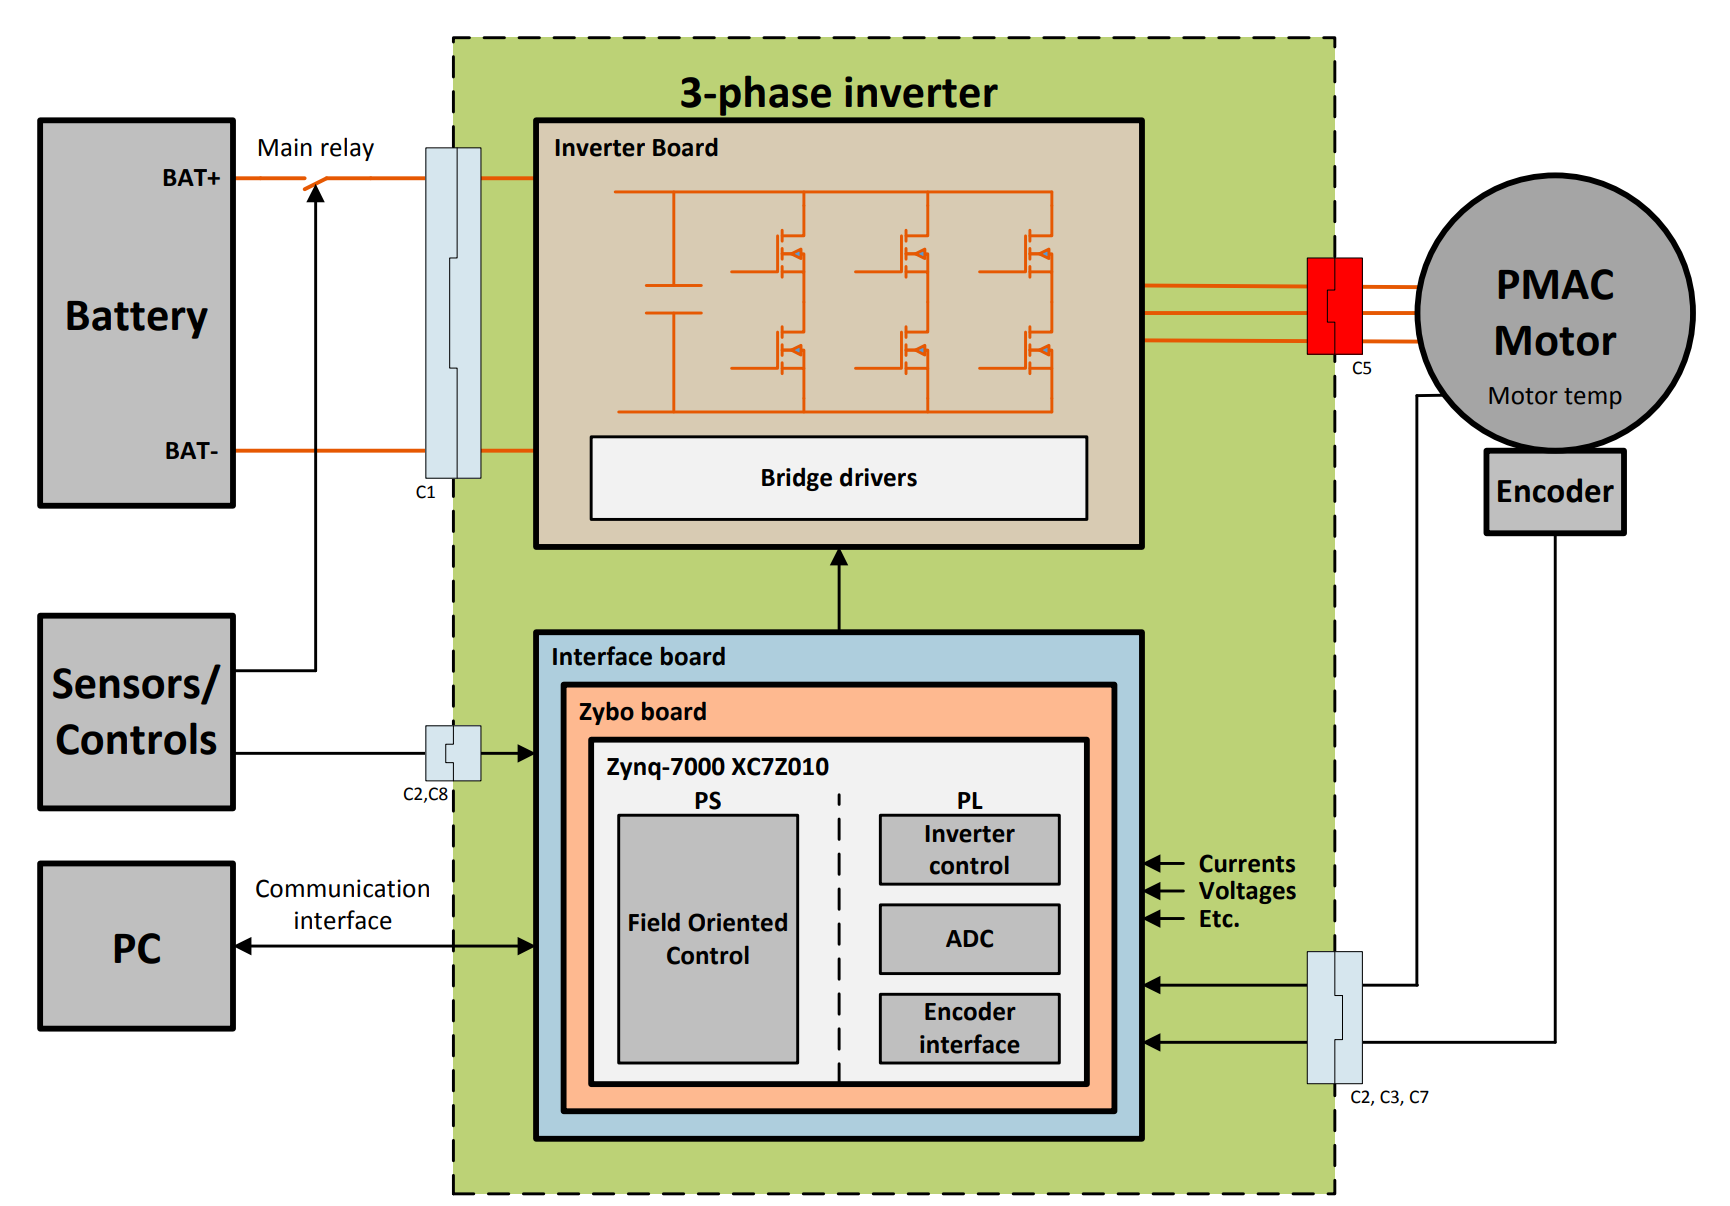
\includegraphics[width=\linewidth]{pictures/general/Project1.PNG}
  \caption{A suggestion to a possible solution given in the project description. \cite{Project 1. semester - S19}}
  \label{fig:Possiblesolution}
\end{figure}

The illustration above shows, a simplified version of how the main connections between elements should look. Where the green area show, where the design needs to take place. The hardware parts is in the 3-phase inverter and a small analog board, with the software being written on a Zybo board micro-controller. The interface board is a component all ready done, it is not designed but the group, but a tool for the communication between hardware and software.

\subsection{Requirements}

\textbf{Project requirement} \\
\textit{Note: Some of the below requirements are taking from the project description, while some are the groups own.} \cite{Project 1. semester - S19}

\begin{itemize}
\item The solution must use a Zynq FPGA and a self‐designed 3‐phase inverter to control the PMAC motor.

\item There should be a control circuit, with a model of the motor and it's controllers.

\item It should be possible to set and get relevant parameters through a communication interface by a computer. 

\item It is not allowed to change any mechanical or electrical parts on the kart, except replacing the Sevcon gen4 controller. 

\end{itemize}

\newpage
% Analysis, Design & Implementation
% Hardware
\section{Hardware}
\label{sec:hardware}

\subsection{Main interface board}

\subsubsection{Encoder}

On the motor is an \textit{AM256} magnetic 8 bit encoder mounted. The encoder is supplied from the main interface board and the signal are routed from the encoder to the Zybo. 

The decoding and translation of the encoder signal are done in the Zybo which is discussed in section \ref{sec:encoder}.

\todo{Insert reference}


\subsection{Analog interface board}
A smaller part of the hardware design is an analog board with two main functions. Convert the analog signal from the current transducers and the torque sensor into signals between $0V$ and $1V$ for the build in ADC's on the controller.

\subsubsection{Current transducer}
The current transducer used is the \textit{LF 205-S}. The transducer has the conversion ratio $1:2000$, which means when the maximum current, $\pm 300A$, passes through, it will give a $\pm 50mA$ signal. To use the ADC's full resolution the signal is converted into a signal going from $0\rightarrow 1$. First the signal is converted to going from $\pm 0.5V$ with a shunt resistor. The size of the shunt is calculated with equation \ref{eq:shunt}.

\begin{equation}
	R = \frac{0.5V}{50mA} = 3.33\Omega
	\label{eq:shunt}
\end{equation}

The resistance is made by setting three $10 \Omega$ in parallel.

The signal is then offset by $+0.5V$, resulting in a signal varying between $0$ and $1V$. The offsetting is done using a \textit{AD620A} instrumentation amplifier with an offset input. The two $R_g$ ports are left open, which will give unity gain on the output.

\begin{figure}[H]
	\centering
	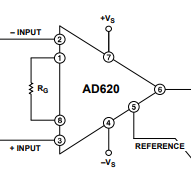
\includegraphics[width=0.4\textwidth]{pictures/hardware/Analog_Interface_board/AD620A.PNG}
	\caption{Instrumentation amplifier AD620A}
	\label{fig:AD620A}
\end{figure} 

The input reference to the \textit{AD620A} has to be very exact. Small differences can cause great inaccuracies in the current measuring. Therefore a voltage reference is used to keep a stable voltage at $0.5V$. The used voltage reference used is a \textit{LM385Z-1.2} in conjunction with a voltage divider of resistors $R1 = 1k\ohm$, $R2 = 1k\ohm$, $R3 = 470\ohm$ yields a constant voltage of

\begin{equation}
	V = V_{ref} \cdot \frac{R1}{R1+R2+R3} = 0.5V
\end{equation}

where 

\begin{equation}
V_{ref} = 1.235V
\end{equation}

A buffer is added to give a low impedance signal to the \textit{AD620A}.

At the input of the instrumentation amplifier a resistor is placed at both the inverting and the non-inverting input to reduce current. Using the \textit{AD620A} is also advantageous for its high CMRR (Common-mode Rejection ratio) that helps with cancelling out noise present on both input pins with the same waveform. It can also use the $\pm15V$ dual supply present on the board.

\subsubsection{Torque pedal measurement}
The output of the torque pedal connects to the same ADC as one of the current channels, hence it also has to be in the range of $0-1V$. The pedal is basically a $7.5k\ohm$ potmeter, so the idea is to parallel it with the lower resistor of a voltage divider to get about $1V$ at full range. Using $V_{ref_3} = 3.3V$ as excitation for the divider and $R1 = R2 = 10K\ohm$, the following equation is true at full throttle: 

\begin{equation}
	V = V_{ref_3} \cdot \frac{R_{pot} \cdot R15}{R_{pot} \cdot R15 + R14} = 0.99V
\end{equation}

When the pedal is not pressed at all, the $0\ohm$ of the potmeter shunts the supply to the ground.

\begin{figure}[H]
\centering
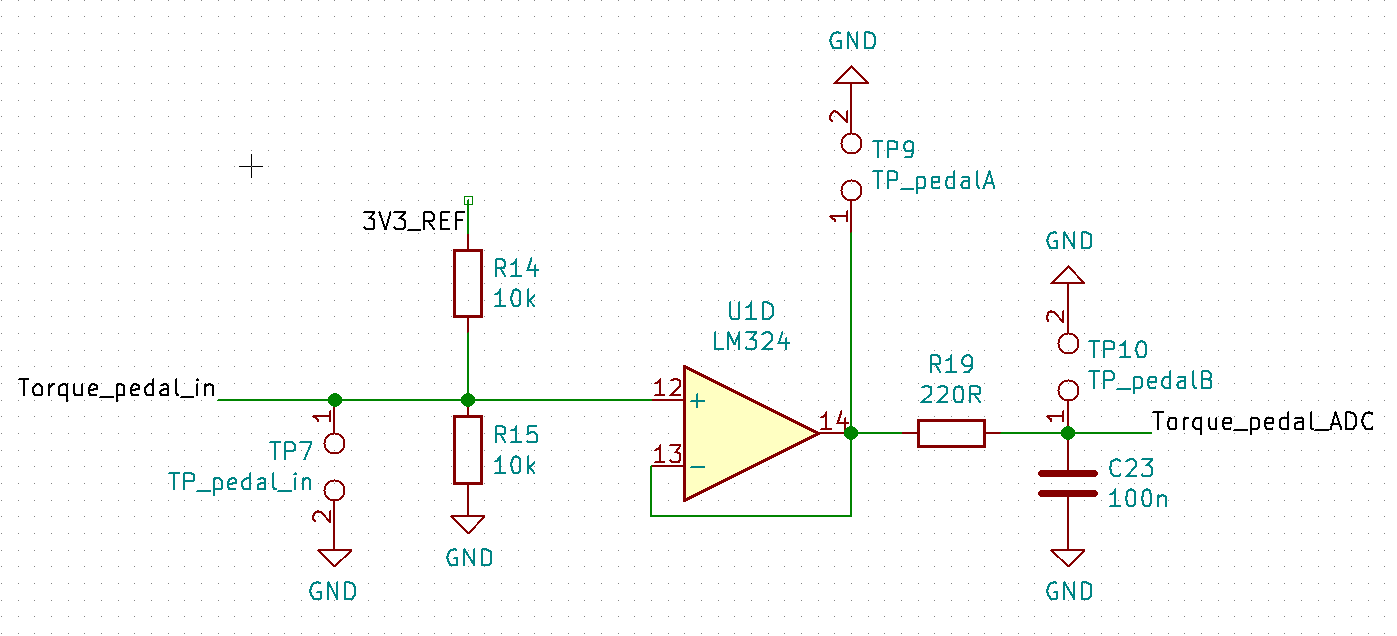
\includegraphics[width=1\linewidth]{pictures/hardware/Analog_Interface_board/torque_pedal_divider.png}
\caption{Torque pedal reading circuit}
\label{fig:torque_pedal_divider}
\end{figure}

For this channel, an opamp in voltage follower configuration is sufficient instead of an instrument amplifier, since no offsetting is required.

\subsection{Power board}
The inverter is divided into two PC boards, one for the high power part, the Power board and one for the driver part, the Driver board. This section will described how the Power board for the inverters is designed and what considerations have been made. It will describe what kind of PCB and which components has been used and why. The layout of the PCBs will also be described and what considerations has been made. \\
\\
The objective is to design a two level three phase inverter to drive the go-carts PMSM motor. This basically consist of six switches and some capacitance on the DC-link. On figure \ref{fig:Sketch_PowerBoard} a simple model of the Power board is shown.

    \begin{figure}[H]
		\centering
		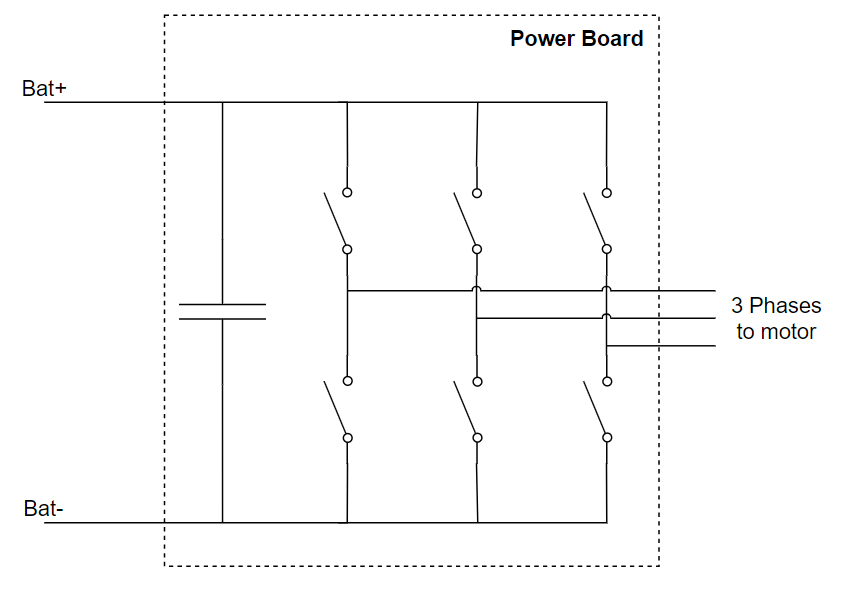
\includegraphics[width=0.7\textwidth]{pictures/hardware/Power_Board/Sketch_of_powerBoard.PNG}
		\caption{Sketch of the Power Board}
		\label{fig:Sketch_PowerBoard}
	\end{figure} 
	
This means that there have to be selected a switch component. The switch component has a great impact on the inverter design, due to that it is a big source of losses in the inverter. It is therefore important to choose a good transistor for switching. Besides the switch component, there has to be selected a type PCB board for the Power board.

\subsubsection{Switching frequency} \label{switching_frequency}
When deciding a switching frequency for the inverters, the rotation frequency of the motor and the thus the frequency of the electrical field.
It is known form the Data sheet of the motor, that the maximum rotation speed of the motor is $5000 rpm$ and it has 8 poles equal to 4 pole pairs. From this the maximum frequency of the electrical field be determined.

\begin{equation}
    f = \frac{v_{rpm} \cdot P}{60}
    \label{eq:max_frequency}
\end{equation}

Where $v_{rpm}$ is the rotational speed in $rpm$ and $P$ is the number of pole pairs in the motor.
From equation \ref{eq:max_frequency} the maximum frequency of the electrical field is $333.3 Hz$.
It is desired to have between 10 and 20 switch periods per period of the electrical field. 20 switch periods per electrical field period results in a switching frequency of $6666 Hz$. It is not necessary to switch faster than the $6666 Hz$, but it is decided to use a switching frequency of $10 kHz$. This is done to make the use of smaller capacitors possible and because already so low frequency it is not a problem to increase it a bit.
It is decided not to increase the switching frequency to more than $10 kHz$ to reducing the switching losses.


\subsubsection{PCB selection}   \label{PCB_selection}
Two types of PCB's has been considered, a ordinary multi-layer PCB and a single-layer aluminum PCB. There is of course pros and cons for both options. With the ordinary PCB there is better opportunities for conducting the heat away from the switch components. On the other hand it is not possible to use SMD components, due to the heat can not be transferred away from the components. The SMD components can result in a better and more compact layout. This is due to the SMD components is smaller and is available with multiple source legs, which minimize the common source for the switch components. The Use of SMD components will be possible with the aluminum PCB. Due to that the SMD components have a smaller area and the heat has the transferred through the aluminum PCB, the cooling of the components is a harder task. With the aluminum PCB it is not possible to use through hole components, which can have some cons when it comes to the mounting of the large capacitors for the DC-link. 

 The ordinary PCB has also the benefit, that is has multiple layers. This could make it easier to layout a good power board. On the other hand, due to the budget, it will not be possible to get a PCB with much more than 2 layers anyways, maybe 4 layers. It is of course better than the single layer on the aluminum PCB. It is possible to get the aluminum PCB with two layers, but it will result in a  too high thermal resistance and price.

Based on these considerations it is chosen to use the aluminum PCB, because the benefits of the SMD components is weighted higher than the cons.


\subsubsection{Transistor selection}
Transistors selection is an important aspect in the design of the inverter. This due to that the transistors has great affect on the power loss in the system and thus the heat dissipation which set the limits of the design. Transistor selected is made from a couple of aspects. first of all the needed ratings necessary for the system. The Drain to Source current has to be rated for $300 A$ if no parallel devices is used. It is chosen that it has to have a rated Drain to Source voltage of $100 V$. This is due to the battery in the go-kart has a maximum voltage of $57.6$ plus some safety margin for voltage spikes. The maximum battery voltage is found based on the cell voltage of a $LiFePO_4$: $3.6 V$, multiplied with the number of cells, which is 16. The transistor has to have a fall time of less than $250ns$ and rise time of less than $50ns$. Besides that the transistor has to have a as low as possible on-resistance, to minimize conduction losses, which is very significance when conducting a current of $300A$.

The Transistor with these specifications and the lowest possible Drain-Source on resistance, to a affordable price, was a MOSFET. The MOSFET have the benefit of having a low current needed for turn on, the ability to handle high current needed for the motor and fast enough for the switching frequency. Since price is everything, when it comes to choice of components, then some sort of compromise will be made \\

The MOSFET chosen is an Infineon "IPB017N10N5". Some of the important specifications is listed in the table below.
\begin{table} [H]
\centering
 \begin{tabular}{|c|c|c|} 
 \hline
 \textbf{Parameters} & \textbf{Value} & \textbf{Unit} \\
 \hline
 \textbf{$V_{DS}$} & $100$ & $V$ \\  
 \hline
 \textbf{$R_{DS-ON}$} & $1.7$ & $m\Omega$ \\
 \hline
 \textbf{$I_D$} & $273$ & $A$ \\
 \hline
 \textbf{$Q_G\ (0-10V)$} & $168$ & $nC$ \\
 \hline
 \textbf{$Q_{GD}$} & $34$ & $nC$ \\
 \hline
 \textbf{$Q_{GS}$} & $53$ & $nC$ \\
 \hline
 \textbf{$Q_{sw}$} & $51$ & $nC$ \\
 \hline
 Rise time & $23$ & $ns$ \\
 \hline
 Fall time & $27$ & $ns$ \\
 \hline
\end{tabular}
\caption{Transistor parameters taken from the "IPB017N10N5" datasheet}
\end{table}

When looking at the parameters, a couple of things need to be considered. From the top it can be seen that the Drain-Source voltage is $100 V$, so it is able to handle the kart's battery voltage. Next the  [$I_D$] is not $300 A$ or above, which leads to a design choice of having two or more in parallel. Having more transistors in parallel has the benefit of splits the current up between them, lowering the conduction power loss. Having lower power loss decreases the amount of heat generated, which leads to less risk of overheating. The gate charge is the amount of charge that needs to be delivered to the gate from the driver, in order to turn the transistor on. This parameter needs to be as low as possible same as the Drain-Source resistance, but normally with a low resistance comes higher gate charge and vise versa. In this case is it more important that the Drain-Source on resistance is low rather than the Gate charge is low. This is the case because speed of the turning on and off of the MOSFET is reduced anyway. Besides that the increased driver power losses will not be as significant compared to the increased power losses in a MOSFET with higher Drain-Source on resistance.\\ 


\subsubsection{Power and heat dissipation in the transistors}
There are two types of power losses in the transistors. One is conduction losses, which is caused by the intern resistance in MOSFET between the Drain and the Source, when the MOSFET is conducting. The other one is switching losses, which is caused then the MOSFETs is turning on and off. Based on the power loss calculations the expected heat increase of the MOSFETs can be estimated, which will be used to decide how many MOSFETs in parallel is needed.

\paragraph{Conduction power loss}
When a MOSFET is conducting there will be a power dissipation due to the intern Drain-Source on resistance in the MOSFET. Thus the conduction power loss in the MOSFETs is calculated in the same way as the power loss in a resistor. Equation \ref{eq:ConductionLossMOSFET} describes the conduction power loss for one MOSFET, $P_{con/MOSFET}$.

    \begin{equation}
        P_{con/MOSFET} = \bigg( \frac{I}{N \cdot 2} \bigg) ^2 \cdot R_{DS-ON}
        \label{eq:ConductionLossMOSFET}
    \end{equation}

$I$ is the peak current, $N$ is the number of transistors in parallel per switch, and $R_{DS-ON}$ is the Drain-Source on resistance of the MOSFET.
The peak current is divided by the number of transistors in parallel, to get the current in one MOSFET. Because the current is sinusoidal and the average duty cycle of the PWM over a period is $50 \% $, it is also divided by two to get the current one transistor is conducting.

To calculate the conduction power loss for all the transistors, it is then multiplied with the number of parallel MOSFETs per switch, two for taking both the high and low side into account, and the number of legs in the inverter, which is three.

    \begin{equation}
        P_{con} = \bigg( \frac{I}{N \cdot \sqrt{2}} \bigg) ^2 \cdot R_{DS-ON} \cdot N \cdot 2 \cdot 3
        \label{eq:ConductionLossTot}
    \end{equation}

On figure \ref{fig:ConductionLoss} the relationship between conduction power loss per MOSFET, equation \ref{eq:ConductionLossMOSFET}, and for all the MOSFETs, equation \ref{eq:ConductionLossTot}, is plotted as a function of the number of MOSFETs in parallel. 

    \begin{figure}[H]
		\centering
		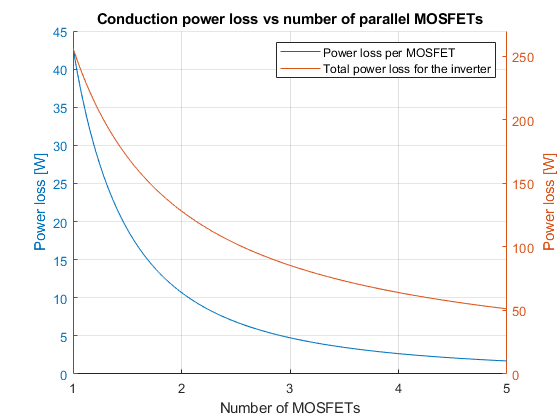
\includegraphics[width=0.8\textwidth]{pictures/hardware/Power_Board/Conduction_loss.png}
		\caption{Conduction power loss versus the number of parallel transistors in parallel per switch}
		\label{fig:ConductionLoss}
	\end{figure} 

For figure \ref{fig:ConductionLoss} the peak current, $I$, is set to $300 A$, and the Drain-Source on resistance, $R_{DSon}$, is set to ${1.9 m \Omega}$, which is value at $80 \degree C$. \todo{ref to data sheet}

On figure \ref{fig:ConductionLoss} it can be seen that the more MOSFETs there are placed in parallel per switch, the conduction power losses reduces exponentially, for both each MOSFET and for the hole inverter.

\paragraph{Switching power loss}
The other cause of power loss in the MOSFETs is the switching power loss. The switching power losses is caused by the period, when switching, where both the voltage over and the current through the MOSFET is not zero. This is called hard switching. Soft switching is when the MOSFET switching on or off without the voltage and current overlaps. This will not cost any power loss. This is illustrated on figure \ref{fig:HardSoftSwitch}.

    \begin{figure}[H]
		\centering
		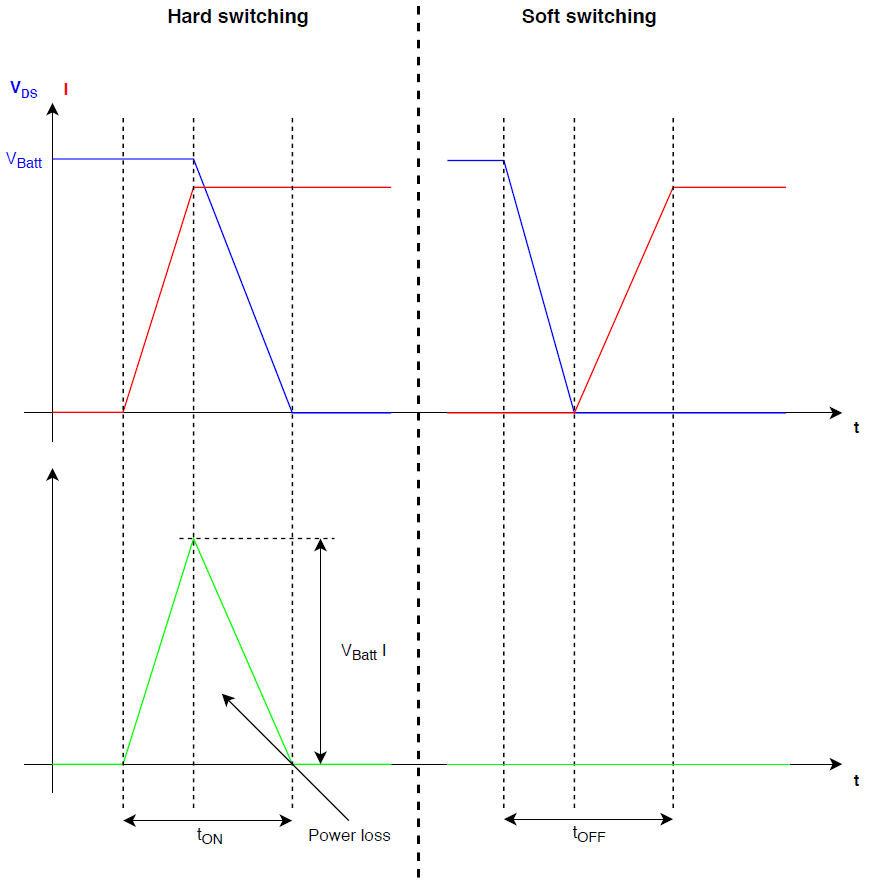
\includegraphics[width=0.8\textwidth]{pictures/hardware/Power_Board/Hard_soft_switching.PNG}
		\caption{Illustration of hard and soft switching of MOSFET}
		\label{fig:HardSoftSwitch}
	\end{figure} 

When running the motor, the motor current has a positive and a negative half cycle. During the positive half period the current going into the motor, and in the negative half period the current going from the motor into the inverter. In the positive half period the low-side switch gets soft turned on and the high-side switch gets hard turned on. Opposite in the negative half period the low-side switch is hard turned on and the high-side switch is soft turned on. This means One transistor will only hard switch $50 \%$ of the time.

The switching power is calculated as the area under the green line on figure \ref{fig:HardSoftSwitch} multiplied with the switching frequency. This is multiplied with a half because the switches is only hard switched $50 \%$ of the time, and therefore the Power loss is the half. 

    \begin{equation}
        P_{sw/MOSFET} = 0.5 \cdot 0.5 \cdot V_{batt} \cdot \frac{I}{N} \cdot (t_{on}+t_{off}) \cdot f_{s}
        \label{eq:sw_loss_MOSFET}
    \end{equation}

Where $V_{batt}$ is the battery voltage, $t_{on}$ is the turn on time, $t_{off}$ is the torn off time, and $f_{s}$ is the switching frequency of the transistors.
Equation \ref{eq:sw_loss_MOSFET} is the switching power loss per MOSFET. To get the switching power loss for all of the MOSFETs in the inverter, this has to be multiplied with the number of parallel MOSFETs, two to take both the high- and low-side into to account, and the number of phases, which is three.

    \begin{equation}
        P_{sw} = 0.5 \cdot 0.5 \cdot V_{batt} \cdot \frac{I}{N} \cdot (t_{on}+t_{off}) \cdot f_{sw} \cdot N \cdot 2 \cdot 3
        \label{eq:sw_loss}
    \end{equation}
    
From this equation, a curve of the switching power loss in one MOSFET and in all the MOSFETs versus the number of the parallel MOSFETs, is made.

    \begin{figure}[H]
		\centering
		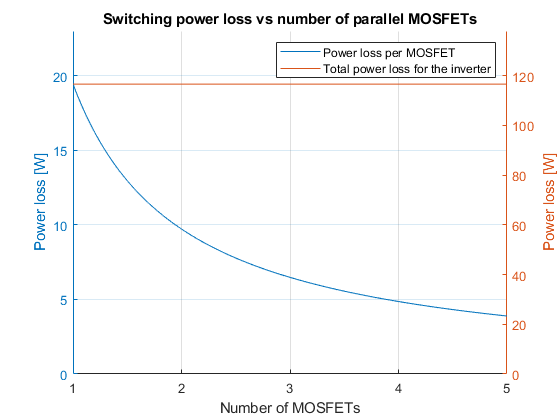
\includegraphics[width=0.8\textwidth]{pictures/hardware/Power_Board/Switch_loss.png}
		\caption{Conduction power loss versus the number of parallel transistors in parallel per switch}
		\label{fig:sw_loss}
	\end{figure}
	
Again is the peak current, $I$, is set to $300 A$. The battery voltage, $V_{batt}$, is set to $57.6 V$ and the switching frequency is set to the chosen frequency: $10 kHz$. The turn on time, $t_{on}$, and the turn off time, $t_{off}$, is calculated with the following equations.

    \begin{equation}
        t_{on} = \frac{Q_{sw}}{I_{GSource}}
    \end{equation}
    
    \begin{equation}
        t_{off} = \frac{Q_{sw}}{I_{GSink}}
    \end{equation}
    
Where $Q_{sw}$ is the switching charge of the MOSFET, which is stated in the Data sheet.\cite{mosfet}
$I_{GSource}$ and $I_{GSink}$ is respectively the current the driver deliverers to the Gate of the MOSFET when turning the MOSFET on and off. These are calculated in section \ref{sec:DriverDesign}. The turn on and off end up being $75 ns$ and $375 ns$, which could be faster, but is chosen to be limited to this. This is due to reducing high-frequency ringing when switching the MOSFETs. This results in a higher switching power loss, but because the switching loss does not have that big of an impact on the total power loss, due to the low switching frequency, it is not considered a problem.

On figure \ref{fig:sw_loss} it can be seen that the switching power loss of each MOSFET is reduced with number of parallel MOSFETs, but the over all power loss of the inverter is the same independent of the number of parallel MOSFETs.

\paragraph{Heat dissipation}
Now when the conduction power loss and switching power loss is determined compared to the number of MOSFETs, the total power losses is known. From the total power loss in the transistors the heat dissipation, depending on the number of MOSFETs, can be determined.

When determine the heat dissipation of the inverter, all the thermal resistances between the junction of the MOSFET and the ambient has to be specified.
First of all there is the internal junction to case resistance for the MOSFET.
When using the aluminum PCB with the SMD components, the heat has to be transferred through the PCB. This means this adds an extra thermal resistance to the system. The aluminum PCB is divided into three parts, the copper layer, a dielecrical layer for isolating the copper from the aluminum, and the aluminum layer.
Then there is a thin layer of thermal paste to connect the PCB to the heat sink. And the last resistance before the ambient is the heat sink. This is illustrated on figure \ref{fig:thermal_overview}.

    \begin{figure}[H]
		\centering
		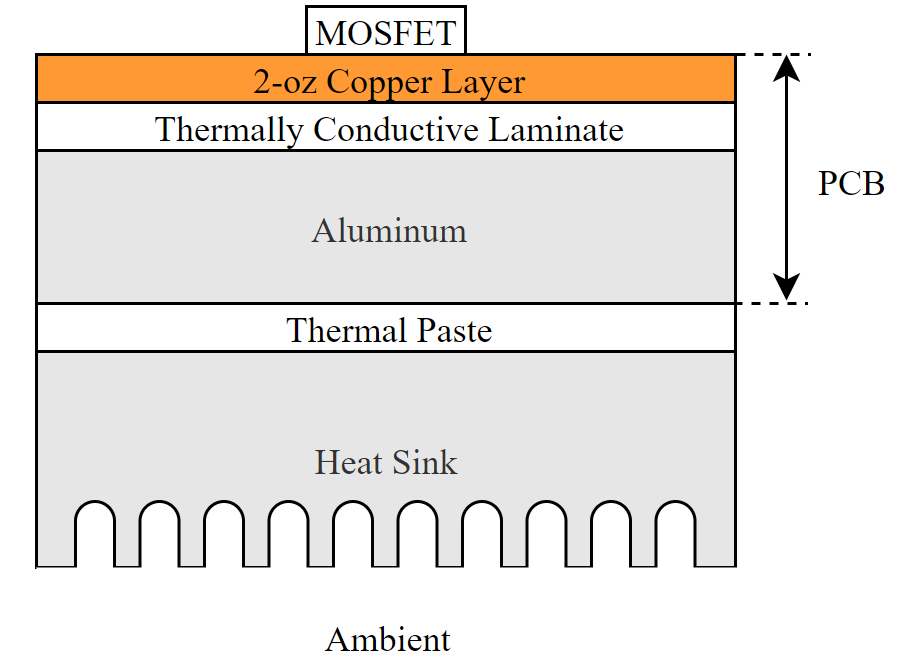
\includegraphics[width=0.6\textwidth]{pictures/hardware/Power_Board/Thermal_overview.png}
		\caption{Overview of the thermal resistances between the junction of the MOSFET and ambient}
		\label{fig:thermal_overview}
	\end{figure}
	
The thermal resistance from the junction to the case of the MOSFET is stated to be $0.4 K/W$ in the data sheet for the MOSFET.\cite{mosfet}
The thermal resistance of the copper layer, is calculated from equation \ref{Rthermal}

    \begin{equation}
        R_{thermal} = \frac{t_{layer}}{A_{MOSFET} \cdot k_{material}} 
        \label{Rthermal}
    \end{equation}
    
Where $t_{layer}$ is the thickness of the layer in $m$, $A_{MOSFET}$ is the surface area of the MOSFET in $m^2$, and $k_{material}$ is the thermal conduction constant for the layer material in $\frac{W}{m \cdot K}$.

The thickness of the copper layer is known to be $1 oz/foot^2$ from 'pcbway.com', which is converted to $34 \cdot 10^{-6} m$ from the density of copper. The area of the surface area of the MOSFET is found in the data sheet to be $63 \cdot 10^{-6} m^2$.\cite{mosfet} The area of the MOSFET is used all the way down to the heat sink, because it is assumed that the heat will go straight through the PCB and the paste. This is most likely not the case but that will be the worst case.
The thermal conduction constant of copper is $401 \frac{W}{m \cdot K}$.\cite{toolbox}

The thermal resistance of the dielectrical layer is calculated based on the same equation as \ref{Rthermal}.

Where the thickness of the dielectrical layer is $100 \mu m$, which is stated by the manufactore, pcbway.com. The thermal conduction constant is chosen to be $1 \frac{W}{m \cdot K}$. The manufacture offers also the aluminum PCB with a dielectrical layer with a thermal conduction constant of $2 \frac{W}{m \cdot K}$, but due to price this was not chosen.

Equation \ref{Rthermal} is used again for calculating the thermal resistance of the aluminum layer of the PCB.
Where the he thickness of the aluminum layer is the chosen PCB thickness of $0.8 mm$ minus the thickness of the two other layers. The thickness of $0.8 mm$ is chosen because that is the thinnest option without getting the PCB more expensive. The thermal conduction constant for aluminum is $236 \frac{W}{m \cdot K}$.\cite{toolbox}

The thermal resistance for the total PCB is then:

    \begin{equation}
        R_{PCB} = R_{copper} + R_{del} + R_{alu}
        \label{RPCB}
    \end{equation}

Where $R_{copper}$ is the thermal resistance of the copper layer, $R_{del}$ is the thermal resistance of the dielectrical layer, and $R_{alu}$ is the thermal resistance of the aluminum layer.

To calculate the thermal resistance of the thermal paste, equation \ref{Rthermal} is used as well. The thickness of the paste is estimated to be $0.1 mm$ and the thermal conduction constant of the paste is set to $3 \frac{W}{m \cdot K}$. This based on values for different thermal paste, and then a value close to the average of them was chosen.

This results in, that the total temperature difference from the thermal paste to the MOSFET junction can be calculated with equation \ref{eq:tempMOSFET}.

    \begin{equation}
        T_{JP} = P_{loss/MOSFET} \cdot (R_{JC} + R_{PCB})
        \label{eq:tempMOSFET}
    \end{equation}
    
Where $R_{JC}$ is the internal junction to case thermal resistance and $P_{loss}$ is the total power loss for one MOSFET. 

To calculate the temperature difference over the heat sink, the average power loss is used instead of the maximum power loss. This is done because the heat sink has a higher thermal capacitance, and therefore is less reactive to changes in temperature. The average power loss is calculated in the same way as the maximum power loss, but instead of using the maximum current a average current is estimated. The average current is estimated to $75 A$.
From this the temperature difference over the heat sink is calculated, with equation \ref{Theatsink} 

    \begin{equation}
        T_{HA} = P_{Avg} \cdot R_{HA}
        \label{Theatsink}
    \end{equation}

The $P_{Avg}$ is the average power loss for all the MOSFETs and $R_{HA}$ is the thermal resistance of the heat sink. 


% \subsubsection{Design}

The $V_{DS}$ fall time (the MOSFET switch-in time) is slowed down to $\approx 250ns$ and the rise time (switch-off) is $\approx 50ns$. The required resistor values can be calculated using Equation \ref{eq:i_Gsink_per_fet_1} through Equation !!!. \\

To get the resistor values, first, the sink current must be calculated for the required switch-off time for the individual MOSFETs.

    \begin{equation}
        i_{Gsink/FET} = \bigg( \frac{Q_{GD}}{t_{sw{\_}off}} \bigg)
        \label{eq:i_Gsink_per_fet_1}
    \end{equation}
    
    where
    
    \begin{itemize}
        \item $i_{Gsink/FET}$ is the required switch-off current
        \item $Q_{GD}$ is the gate-drain charge of the MOSFET
        \item $t_{sw{\_}off}$ is the desired switch-off time
    \end{itemize}
    
    \begin{equation}
        i_{Gsink/FET} = \bigg( \frac{V_{Miller}}{R_{G{\_}FET} + R_{G{\_}FET{\_}int}} \bigg)
        \label{eq:i_Gsink_per_fet_2}
    \end{equation} \\
    
    Rearranging Equation \ref{eq:i_Gsink_per_fet_2} yields the following:
    
    \begin{equation}
        R_{G{\_}FET} = \bigg( \frac{V_{Miller}}{i_{Gsink/FET}} - R_{G{\_}FET{\_}int} \bigg)
        \label{eq:i_Gsink_per_fet_2}
    \end{equation}
    
    where
    
    \begin{itemize}
        \item $R_{G{\_}FET}$ is the resistor for the individual MOSFETs
        \item $V_{Miller}$ is the Miller-plateau of the MOSFET
        \item $R_{G{\_}FET{\_}int}$ is the internal gate-source resistance of the MOSFET
    \end{itemize}
    
    Now the common resistance can be calculated:
    
    \begin{equation}
        i_{Gsource/FET} = \frac{\frac{V_G - V_{Miller}}{R_{pullup} + R_G}}{N}
        \label{eq:i_Gsoursce_per_fet_1}
    \end{equation}
    
    where
    
        \begin{equation}
        i_{Gsource/FET} = \frac{\frac{V_G - V_{Miller}}{R_{pullup} + R_G}}{N}
        \label{eq:i_Gsoursce_per_fet_1}
    \end{equation}
    
    Rearranging Equation \ref{eq:i_Gsoursce_per_fet_1} yields the following:
    
    \begin{equation}
        i_{Gsource/FET} = \frac{\frac{V_G - V_{Miller}}{R_{pullup} + R_G}}{N}
        \label{eq:i_Gsoursce_per_fet_1}
    \end{equation}
% \subsubsection{Implementation}

\subsection{Driver board}
This section describes the theoretical background, the design considerations taken and the implementation of the driver circuit and the PCB.
\subsubsection{Analysis}
The gate driver selected for this design is the SI8261BAC-C-IS\cite{Si8261} from Silicon Labs. It is driven by the $3.3V$ output of the Zybo while providing an output of $12V$, constrained by the attached $12V$ floating supply Cosel MGS1R54812\cite{MGS1R5}. A floating supply is required for the high-side to be able to take on a potential independent of the power ground when its drain and source potential is constrained by the load and the battery voltage. The gate driver's ground floats along with the source potential of the FET so it is always able to provide a voltage of $12V$ between the gate and the source. The advantage of having an isolated supply for the low-side as well is better noise tolerance - the FETs reference level is made somewhat independent of the ripple current on the power ground from all the loads. The high-side floating supply also has the advantage over a bootstrap capacitor of not requiring  part of an output cycle to be used for charging the capacitor. This way more power can be used to propel the gokart.

\begin{figure}[H]
	\centering
	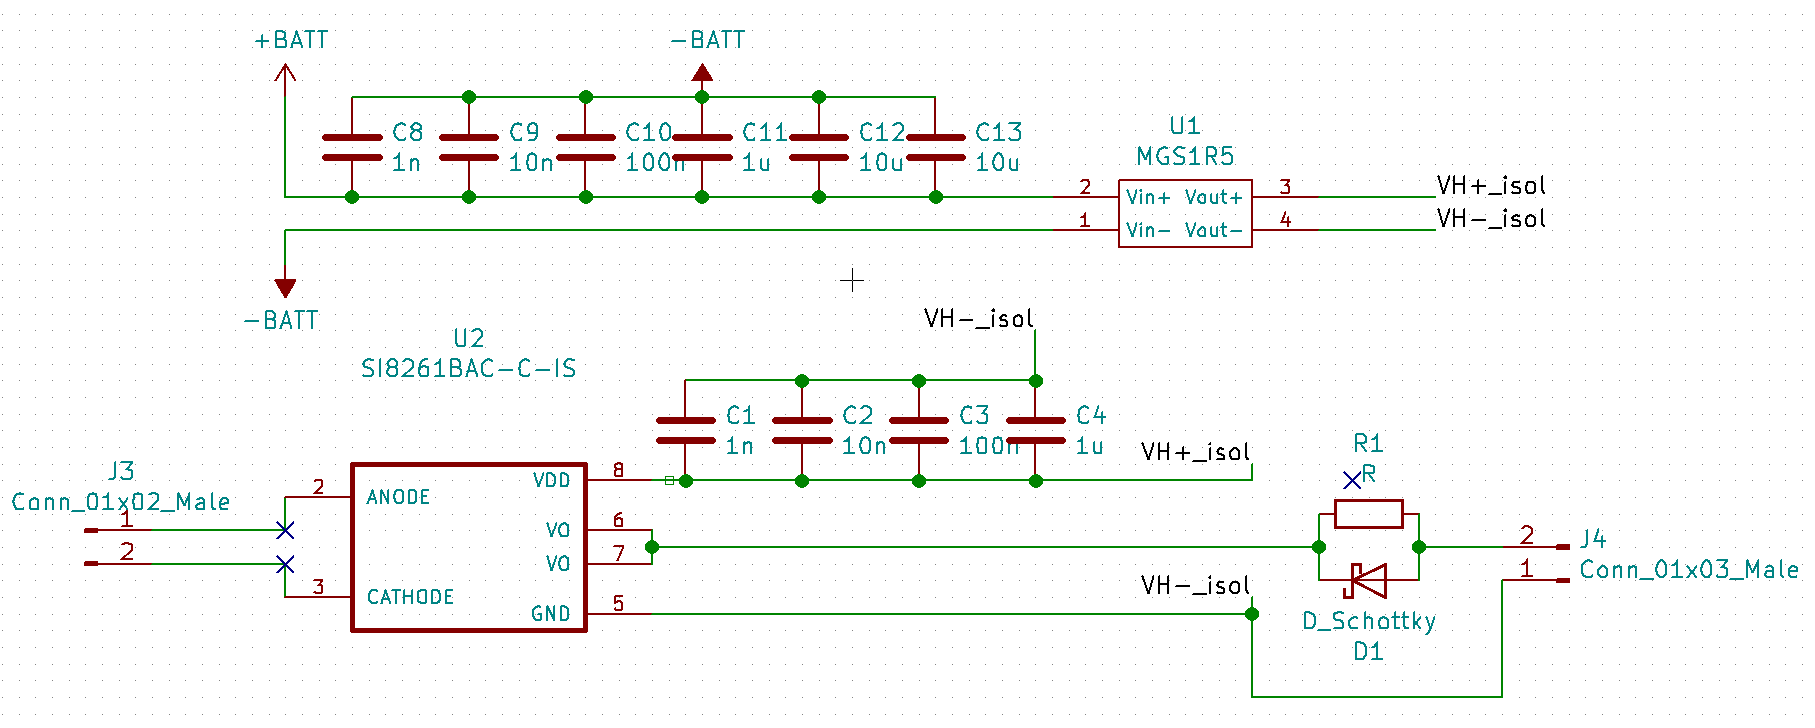
\includegraphics[width=0.6\linewidth]{pictures/hardware/Driver_Board/driver_circuit.png}
	\caption{One leg of one phase of the driver circuit}
	\label{fig:driver_circuit}
\end{figure}

 Figure \ref{fig:driver_circuit} shows the driver of one leg of one phase. Separate drivers were chosen for the separate legs of each phase to reduce the thermal stress of the individual IC-s. The low-side and the high-side driver circuit is identical. \\

A series of capacitors is attached both to the input and output of the floating supply. The smaller ones are meant to serve as high-frequency decouplers while the $10$$\mu$$F$  ones are the bulk capacitors to prevent droop on the $12V_{DC}$ rail. This helps with countering the noise-emitting effects of the long wires and quick transients from the battery when load changes rapidly. \\

The turnon and turnoff times were chosen to be around the slower end of the available range to make the circuit less prone to overshoot and ringing caused by the parasitic inductances and capacitances inherently present in the layout. The analysis of deciding the switching frequency is detailed in section \ref{switching_frequency}. \\

In Figure \ref{fig:CSI_current} and Figure \ref{fig:skew_current} taken from TIDA-00364\cite{TIDA-00364} reference design by TI, the use of split gate resistors can be seen. These consist of R2, which is common to all the parallel MOSFETs, and R20 through 24, which are individual to each MOSFET . R2 helps to easily change the turnon gate current of all the parallel FETs by changing a single resistor instead of changing each of the individual resistors. R20 through R24 help in suppressing the circulating current between the gate of the MOSFETs, which may cause gate voltage ringing. To describe the mechanism, consider only two FETs in parallel as shown in Figure \ref{fig:CSI_current} . Due to the layout, the parasitic common source inductance (CSI) of all the FETs will not be equal. If both the FETs are turned on the same instant and if the di/dt of the drain currents are equal, the voltage across CSI of both FETs (VLs1 and VLs2) will not be equal. This drives a circulating current as shown in Figure \ref{fig:skew_current} . Another possibility is if there is a skew in the $V_{DS}$ rise and fall time of the parallel FETs, circulating current can flow through the $C_{GD}$ as shown in Figure \ref{fig:skew_current} and cause unwanted behavior. Using individual gate resistors help to suppress the circulating current and help damp unwanted ringing effects. Due to a misunderstanding, we failed to place split resistors, only one is placed at the output of the driver IC, parallel to a diode meant to provide quicker turn-off times. In the upcoming sections the case of the split resistors will be further examined, as it was the original plan.

\begin{figure}[H]
	\centering
	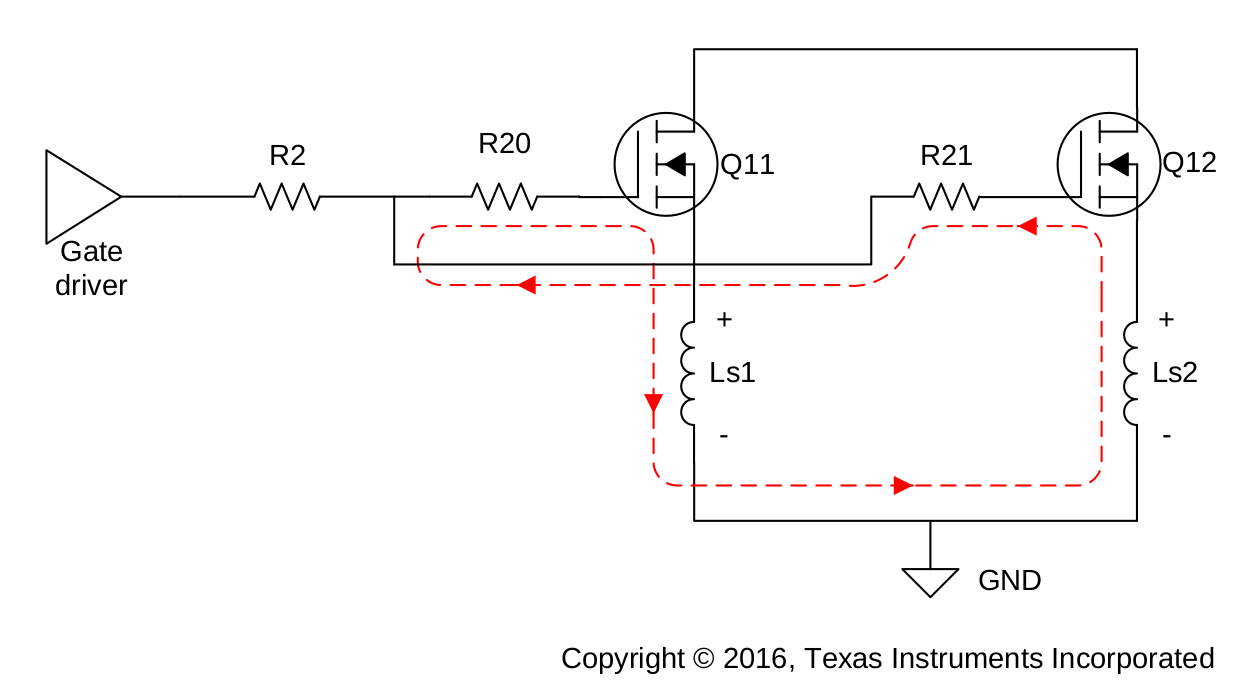
\includegraphics[width=0.6\linewidth]{pictures/hardware/Driver_Board/CSI.png}
	\caption{Gate circulating current due to CSI}
	\label{fig:CSI_current}
\end{figure}

\begin{figure}[H]
	\centering
	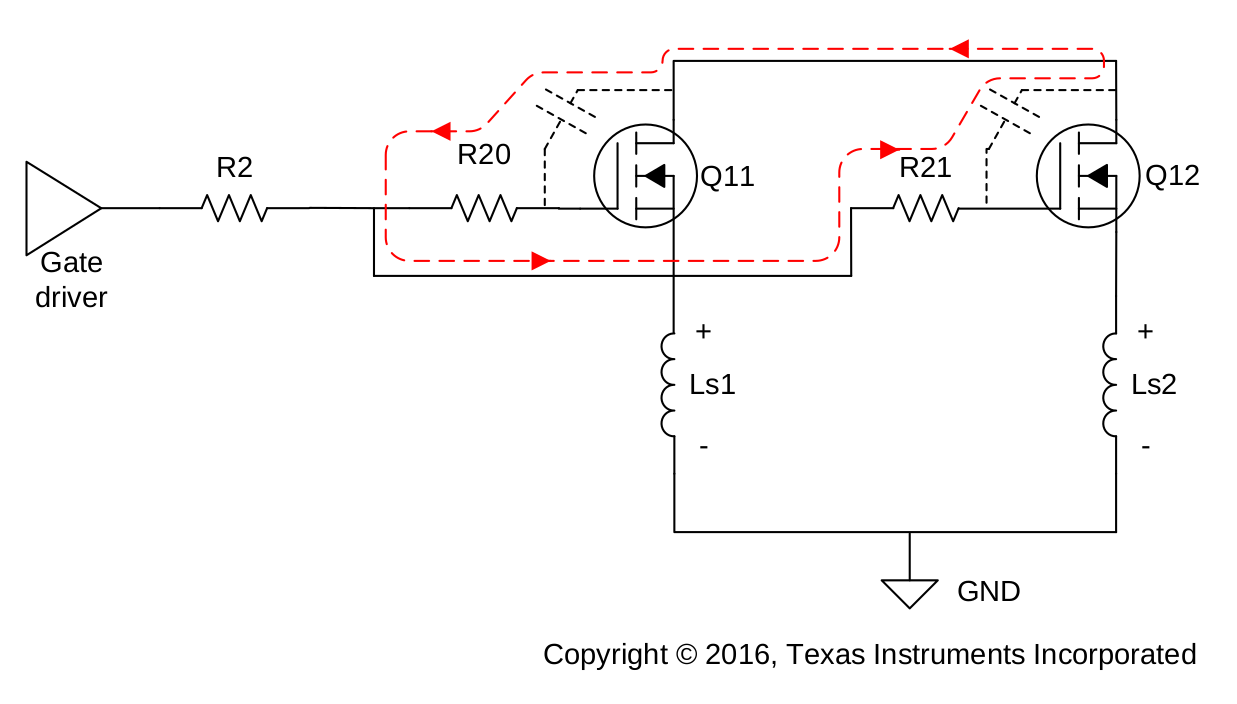
\includegraphics[width=0.6\linewidth]{pictures/hardware/Driver_Board/skew.png}
	\caption{Gate circulating current due to skew}
	\label{fig:skew_current}
\end{figure}
\subsubsection{Design}

The $V_{DS}$ fall time (the MOSFET switch-in time) is slowed down to $\approx 250ns$ and the rise time (switch-off) is $\approx 50ns$. The required resistor values can be calculated using Equation \ref{eq:i_Gsink_per_fet_1} through Equation !!!. \\

To get the resistor values, first, the sink current must be calculated for the required switch-off time for the individual MOSFETs.

    \begin{equation}
        i_{Gsink/FET} = \bigg( \frac{Q_{GD}}{t_{sw{\_}off}} \bigg)
        \label{eq:i_Gsink_per_fet_1}
    \end{equation}
    
    where
    
    \begin{itemize}
        \item $i_{Gsink/FET}$ is the required switch-off current
        \item $Q_{GD}$ is the gate-drain charge of the MOSFET
        \item $t_{sw{\_}off}$ is the desired switch-off time
    \end{itemize}
    
    \begin{equation}
        i_{Gsink/FET} = \bigg( \frac{V_{Miller}}{R_{G{\_}FET} + R_{G{\_}FET{\_}int}} \bigg)
        \label{eq:i_Gsink_per_fet_2}
    \end{equation} \\
    
    Rearranging Equation \ref{eq:i_Gsink_per_fet_2} yields the following:
    
    \begin{equation}
        R_{G{\_}FET} = \bigg( \frac{V_{Miller}}{i_{Gsink/FET}} - R_{G{\_}FET{\_}int} \bigg)
        \label{eq:i_Gsink_per_fet_2}
    \end{equation}
    
    where
    
    \begin{itemize}
        \item $R_{G{\_}FET}$ is the resistor for the individual MOSFETs
        \item $V_{Miller}$ is the Miller-plateau of the MOSFET
        \item $R_{G{\_}FET{\_}int}$ is the internal gate-source resistance of the MOSFET
    \end{itemize}
    
    Now the common resistance can be calculated:
    
    \begin{equation}
        i_{Gsource/FET} = \frac{\frac{V_G - V_{Miller}}{R_{pullup} + R_G}}{N}
        \label{eq:i_Gsoursce_per_fet_1}
    \end{equation}
    
    where
    
        \begin{equation}
        i_{Gsource/FET} = \frac{\frac{V_G - V_{Miller}}{R_{pullup} + R_G}}{N}
        \label{eq:i_Gsoursce_per_fet_1}
    \end{equation}
    
    Rearranging Equation \ref{eq:i_Gsoursce_per_fet_1} yields the following:
    
    \begin{equation}
        i_{Gsource/FET} = \frac{\frac{V_G - V_{Miller}}{R_{pullup} + R_G}}{N}
        \label{eq:i_Gsoursce_per_fet_1}
    \end{equation}

\subsection{Power and Driver board layout}
\subsubsection{Overview}

The proper PCB layout of the driver board is just as essential as that of the power board. To keep the price of the PCBs down, both the power and the driver board has to be kept under $100mm x 100mm$. The layer number of the boards is also a pricey concern. Read more on PCB selection in Section \ref{PCB_selection}. The driver board was designed on 2-layer FR4 1 oz. material. \\

The power board was first laid out to get a precise and optimal placement of the critical components, power rails, outputs and interboard connectors. After that came defining the contour of the driver board, precise placement of interboard connectors and crude placement of components. It is vital for all signals to have their firm ground plane under them to act as reference. That is why the bottom side of the driver board was partitioned according to the components on the top side to have their respective ground planes. The surface of the cooper fills were reduced as much as possible to counter capacitive noise propagation. Supply-ground decoupling capacitors were placed as close to their supported components as possible. 0805 and 1206 size code footprints were placed to have more possibilities for modification or rework if need be. A coutout over the power rails provides space for the electrolitic capacitors attached to the busbar. For approximate mechanical construction, see Figure \ref{fig:mech_top} and Figure \ref{fig:mech_persp}.

\begin{figure}[H]
	\centering
	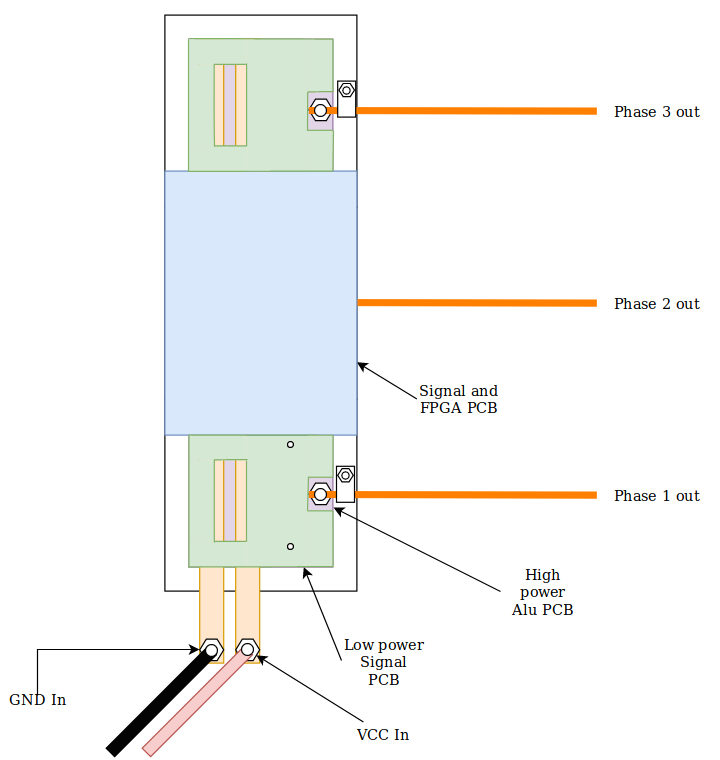
\includegraphics[width=1\textwidth]{pictures/hardware/Power_Board/mechanical_top_new.png}
	\caption{Top view of mechanical construction}
	\label{fig:mech_top}
\end{figure}

\begin{figure}[H]
	\centering
	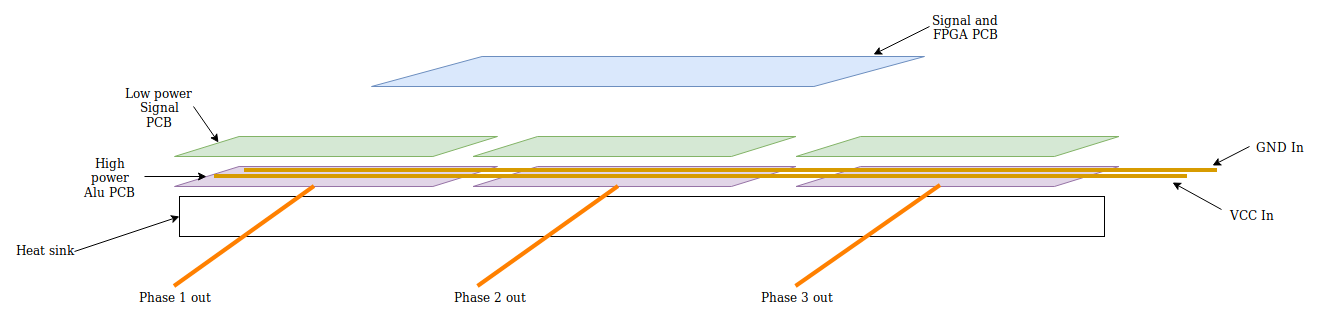
\includegraphics[width=1\textwidth]{pictures/hardware/Power_Board/mechanical_persp_new.png}
	\caption{Perspective view of mechanical construction}
	\label{fig:mech_persp}
\end{figure}

\subsubsection{Power board}

Individual PCBs of $100mm x 65mm$ were chosen for each phase. This way they would be within the general size constraints and fit the $100mm x 200mm$ heatsink that we had available. The three boards are interconnected with the power rail busbars. Only the top side of the alu PCB has a copper layer. This is partitioned into 3 regions. Te first is the battery positive VCC, it is connected to the drain of the high-side MOSFETs. The common region is the output, it gives place to the high-current screw terminal. The source of the low-side FETs is connected to the battery negative GND. To provide the best supply-ground capacitive decoupling and keep the circuit highlighted in \ref{} as short as possible, capacitors are placed along the border of the VCC and GND planes. Electrolitic capacitors sit attached to the busbars. It is important to have as high capacitance ones as possible while keeping the ESR (equivalent series resistance) and stray inductance

\subsubsection{Driver board}


\newpage
% Control
\section{Control}
\label{sec:control}

% The control will be done with vector control also known as field orientated control (FOC) where the motor currents are transformed from three-phase AC signals to a single vector in a rotating dp-frame with a Clarke and a Park transformation. The controller is placed in the dq-frame and its output signals are converted from a rotating vector in the dq-frame back to a signal for each inverter phase.
The section will go through which control type has been chosen, how it works and how it is used. Then the motor model is setup and explained and lastly the motor controller is designed.

\subsection{Simplified motor model}
The motor is a \textit{Motenergy ME1117 PMAC Motor}. Its parameters can be seen in table \ref{Motor_parameters_list}.

\begin{table} [H]
    \centering
    \begin{tabular}{|c|c|} \cline{1-2}
        \textbf{Parameters} & \textbf{Number} \\ \cline{1-2}
        \textbf{Pole pair} & $4\ pairs\ (8\ poles)$ \\ \cline{1-2}
        \textbf{Phase to Phase R} & $0.013\ohm$ \\ \cline{1-2}
        \textbf{Maximum rotational speed} & $5000$ \textit{RPM} \\ \cline{1-2}
        \textbf{Voltage rating} & $0-76$ \textit{Volts} \\ \cline{1-2}
        \textbf{Torque constant} & $0.13$ \textit{Nm/A} \\ \cline{1-2}
        \textbf{Inductance Phase to Phase} & $0.1$ \textit{mH} \\ \cline{1-2}
        \textbf{Armature Inertia} & $52\ kg/cm^2$ \\ \cline{1-2}
        \textbf{Continuous current} & $100\ A$ \\ \cline{1-2}
        \textbf{Peak Current for 1 min} & $300\ A$ \\ \cline{1-2}  
    \end{tabular} \\
    \caption{Motor parameters as seen in \cite{Motor_Parameters}}
    \label{Motor_parameters_list}
\end{table} 

All of these specifications are what makes up the motor, and will be written into the model motor. It will also be used in order to calculate framework of the controller. Before diving in to the specifics of how and why, certain methods is used. A quick overview of the base model, will help visualize how the final model was made.\\

\begin{figure} [H]
    \centering
    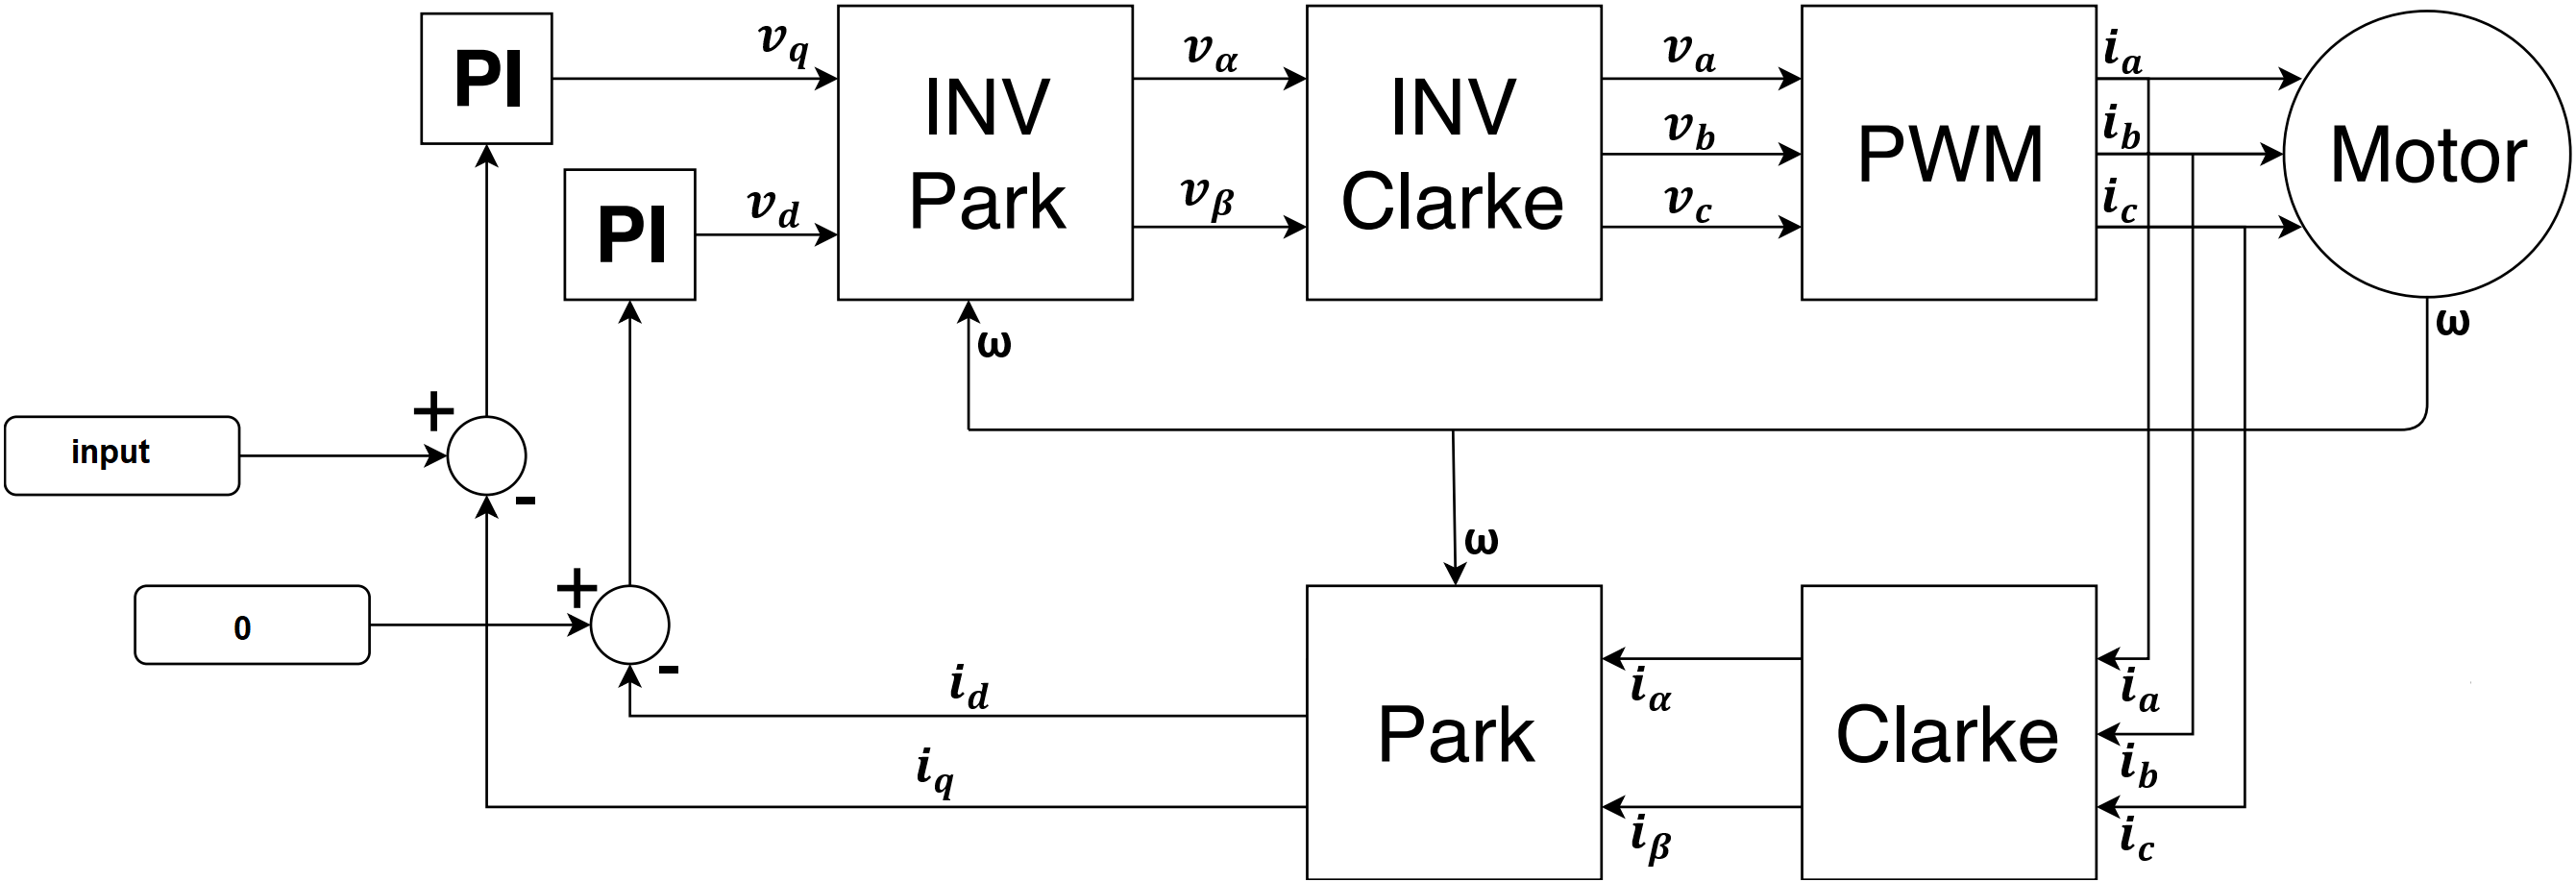
\includegraphics[scale=0.42]{pictures/control/udklip.PNG}
    \caption{Motor model used for the control as an overview.}
    \label{fig:Motor_model}
\end{figure} 

As seen in \ref{fig:Motor_model} the model consist of two inputs, two PI controllers, and inverse Park and Clarke transformations, a motor with the data from \ref{Motor_parameters_list} and negative feedback transformed back with normal Park, Clarke transformation.\\

The general idea behind model is having the input, being the wanted speed of the motor as a current, in go karts case it would be the torque pedal. The $0$ input is $0$ because of field oriented control, more on that in next section. The signal is then being tuned with the negative feedback and the controllers. Having the signal transformed is an important step, since a 3-phase motors needs 3 signals. The PWM box adjust the actual speed of the motor. The feedback comes from the 3 phases and the speed, that all help minimize errors in the signal. \\

\subsubsection{Field oriented control}
There is in motor control, a couple of common techniques used. The calculations are usually scalar based or vector based, each having their usages. In this project the technique used is FOC, which is vector based. \\

\begin{figure} [H]
    \centering
    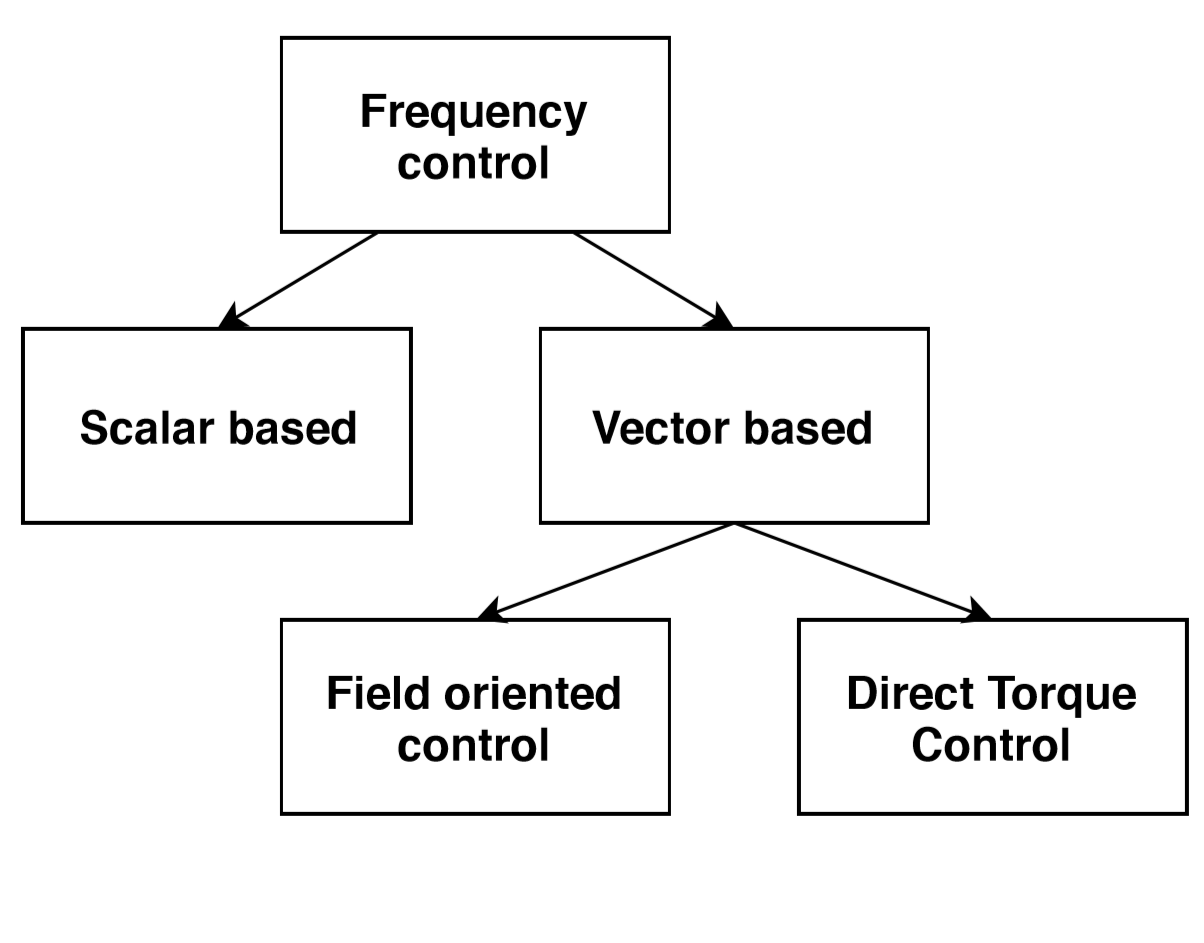
\includegraphics[scale=0.6]{pictures/control/udklip1.PNG}
    \caption{An overview of where FOC is lays among frequency control}
    \label{fig:my_label}
\end{figure} 

The reason for using FOC in this given project, is because it is relatively easy to use and implement. This method gives control over the current and voltages, and gives information about the orientation of the rotor, which gives smoother operation of the motor than normal PWM control. \\

\begin{figure} [H]
    \centering
    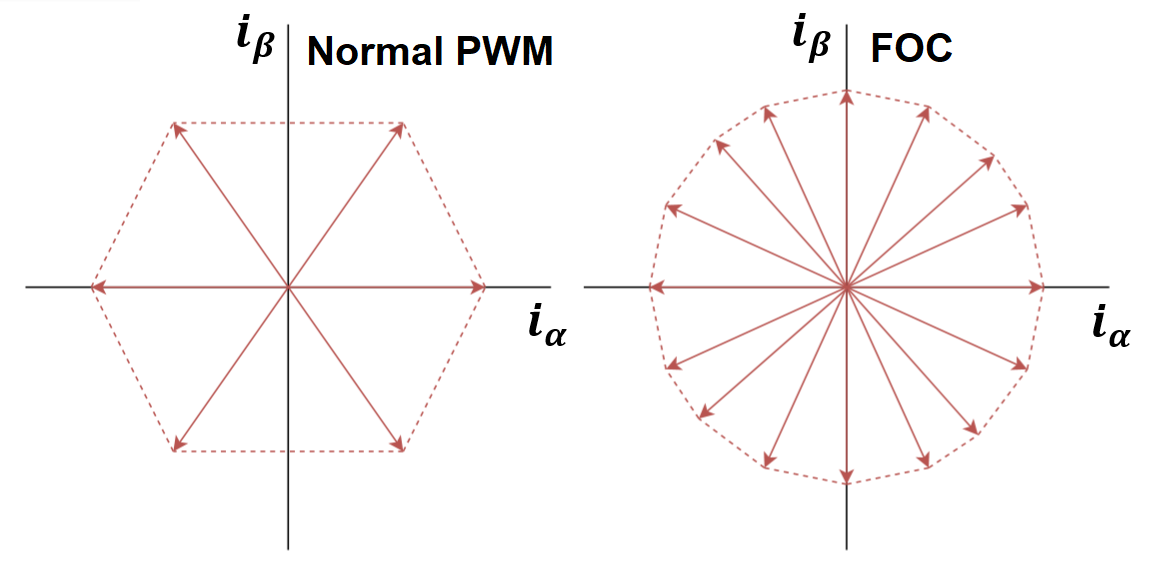
\includegraphics[scale=0.85]{pictures/control/Udklip2.PNG}
    \caption{A visualization of how FOC gives higher control of the PWM signal, the red line representing more steps of where the magnetic field can be placed.}
    \label{fig:my_label}
\end{figure}




\subsection{Clarke and Park Transformations}




% ************************** Clarke Transformation ***********************************
\subsubsection{Clarke Transformation}
The Clarke transformation converts three rotating phase currents to one rotating vector in the alpha-beta frame. The Clarke transformation is performed by using the two equations \ref{eq:clarke_transformation}.

\begin{equation}
    i_{\alpha} = \frac{2}{3} \cdot i_a - \frac{1}{3} \cdot i_b - \frac{1}{3} \cdot i_c
    , \hspace{1cm}
    i_{\beta} = 0 \cdot i_a + \frac{1}{\sqrt{3}} \cdot i_b - \frac{1}{\sqrt{3}} \cdot i_c
    \label{eq:clarke_transformation}
\end{equation}

It can also be written in matrix form as in equation \ref{eq:CtransMatrix}. 

\begin{equation}
    \centering
    \begin{bmatrix}
        i_{\alpha} \\ 
        i_{\beta}
    \end{bmatrix}
    =
    \begin{bmatrix}
        \frac{3}{2} & -\frac{1}{3} & -\frac{1}{3} \\
        0 & \frac{1}{\sqrt{3}} & -\frac{1}{\sqrt{3}} \\
    \end{bmatrix}
    \begin{bmatrix}
        i_{a} \\ 
        i_{b} \\ 
        i_{c}
    \end{bmatrix}
    \label{eq:CtransMatrix}
\end{equation}


% ************************** Park Transformation ***********************************
\subsubsection{Park Transform}
To convert the one rotating vector in the alpha-beta frame to a static vector in the rotating dp-frame, the Park transformation is used. The park transformation is performed with equtation \ref{eq:park_transformation}.

\begin{equation}
    i_{d} = cos(\varphi) \cdot i_{\alpha} + sin(\varphi) \cdot i_{\beta}
    , \hspace{1cm}
    i_{q} = -sin(\varphi) \cdot i_{\alpha} + cos(\varphi) \cdot i_{\beta}
    \label{eq:park_transformation}
\end{equation}

Where
$\omega t = \varphi$

\begin{equation}
    \centering
    \begin{bmatrix}
        i_{d} \\ 
        i_{q}
    \end{bmatrix}
    =
    \begin{bmatrix}
       cos(\omega t) & sin(\omega t) \\
       -sin(\omega t) & cos(\omega t)
    \end{bmatrix}
    \begin{bmatrix}
        i_{\alpha} \\ 
        i_{\beta}
    \end{bmatrix}
\end{equation}





% ************************** Inverse Park Transformation ***********************************
\subsubsection{Inverse Park Transform}
Converts a static vector in a rotating dq-frame into a rotating vector in a alpha-beta frame.

\begin{equation}
    \centering
    \begin{bmatrix}
        i_{\alpha} \\ 
        i_{\beta}
    \end{bmatrix}
    =
    \begin{bmatrix}
       cos(\omega t) & -sin(\omega t) \\
       sin(\omega t) & cos(\omega t)
    \end{bmatrix}
    \begin{bmatrix}
        i_{d} \\ 
        i_{q}
    \end{bmatrix}
\end{equation}

Where
$\omega t = \varphi$

\begin{equation}
    i_{\alpha} = cos(\varphi) \cdot i_{d} - sin(\varphi) \cdot i_{q}
    , \hspace{1cm}
    i_{\beta} = sin(\varphi) \cdot i_{d} + cos(\varphi) \cdot i_{q}
    \label{eq:inverse_park_transformation}
\end{equation}

% ************************** Inverse Clarke Transformation ***********************************
\subsubsection{Inverse Clarke Transform}
Converts a rotating vector in the alpha-beta frame into three phase signals. 

\begin{equation}
    \centering
    \begin{bmatrix}
        i_{a} \\ 
        i_{b} \\ 
        i_{c}
    \end{bmatrix}
    =
    \begin{bmatrix}
        1 & 0 \\
        - \frac{1}{2} & \frac{\sqrt{3}}{2} \\
        - \frac{1}{2} & - \frac{\sqrt{3}}{2}
    \end{bmatrix}
    \begin{bmatrix}
        i_{\alpha} \\ 
        i_{\beta}
    \end{bmatrix}
\end{equation}


\begin{equation}
    i_{a} = i_{\alpha}
    , \hspace{1cm}
    i_{b} = -\frac{1}{2} \cdot i_{\alpha} + \frac{\sqrt{3}}{2} \cdot i_{\beta}
    , \hspace{1cm}
    i_{c} = -\frac{1}{2} \cdot i_{\alpha} - \frac{\sqrt{3}}{2} \cdot i_{\beta}
    \label{eq:inverse_clarke_transformation}
\end{equation}

\subsection{Motor model}
A model of the motor needs to be made for the system model. The motor is a PMSM,  which means that it is driven by three phase currents. To simplify the model, the equivalent circuit for the d- and q-directions are drawn, and a model is made, based on those. In that way the PMSM can be controlled like an DC-machine.

\subsubsection{Motor model in the d-direction}
The equivalent circuit for the d-direction voltage $v_d$ of the PMSM is shown on figure \ref{fig:vd}.

\begin{figure}[H]
	\centering
	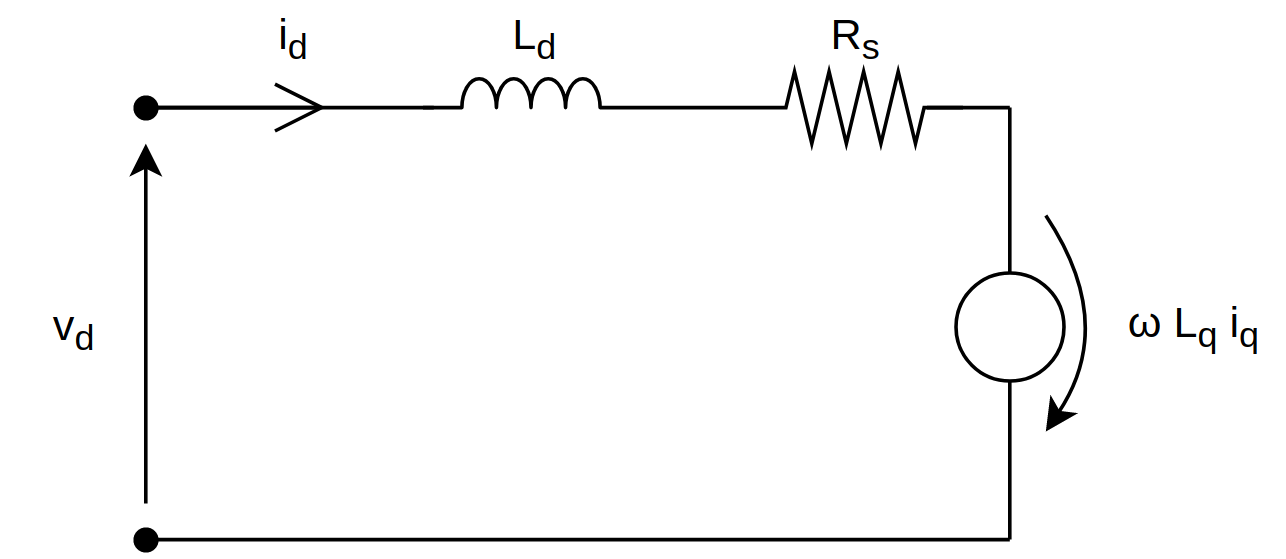
\includegraphics[width=0.6\linewidth]{pictures/control/vd}
	\caption{D-dierection equivalent circuit for the PMSM}
	\label{fig:vd}
\end{figure}


From the equivalent diagram the d-direction voltage can be described as in equation \ref{eq:d_direction}.

\begin{equation}
    \label{eq:d_direction}
    v_d = L_d \frac{d i_d}{dt} + R_s i_d - \omega L_q i_q
\end{equation}
% $\varphi_{rq} = L_qi_q$
% \begin{equation}\label{eq:d_direction2}
% v_{d} = \frac{d \varphi_{rq}}{dt} + R_s i_d - \omega \varphi_{rq}
% \end{equation}

$L_d$ and $L_q$ are respectively the d- and q-direction equivalent stator inductances for the motor, $i_d$ and $i_q$ are respectively the d- an q-direction currents, $R_s$ is the stator resistance for the motor, and $\omega$ is the rotational speed of the rotor.

If $i_d$ from the $L_d \frac{di_d}{dt}$ part is isolated and Laplace transformed it result in equation \ref{eq:d_direction}.

\begin{equation}
    \label{eq:d_direction2}
    I_d = \frac{1}{S} \frac{1}{L_d} (V_d - I_d R_d + \omega L_q I_q)
\end{equation}

From equation \ref{eq:d_direction2} the model of the d-direction of the motor is determined. That can be seen on figure \ref{fig:simulink_d_direction}.

\begin{figure}[H]
	\centering
	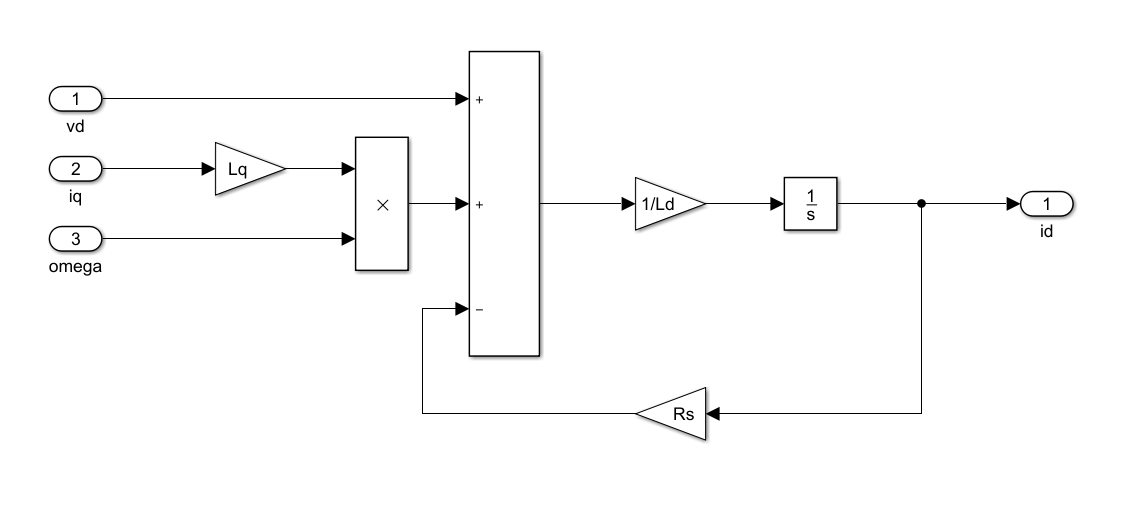
\includegraphics[width=0.8\linewidth]{pictures/control/simulink_d_direction.PNG}
	\caption{Simulink model of the d-direction of the motor model}
	\label{fig:simulink_d_direction}
\end{figure}



\subsubsection{Motor model in the q-direction}
The equivalent circuit for the q-direction voltage $v_q$ is shown on figure \ref{fig:vq}.

\begin{figure}[H]
	\centering
	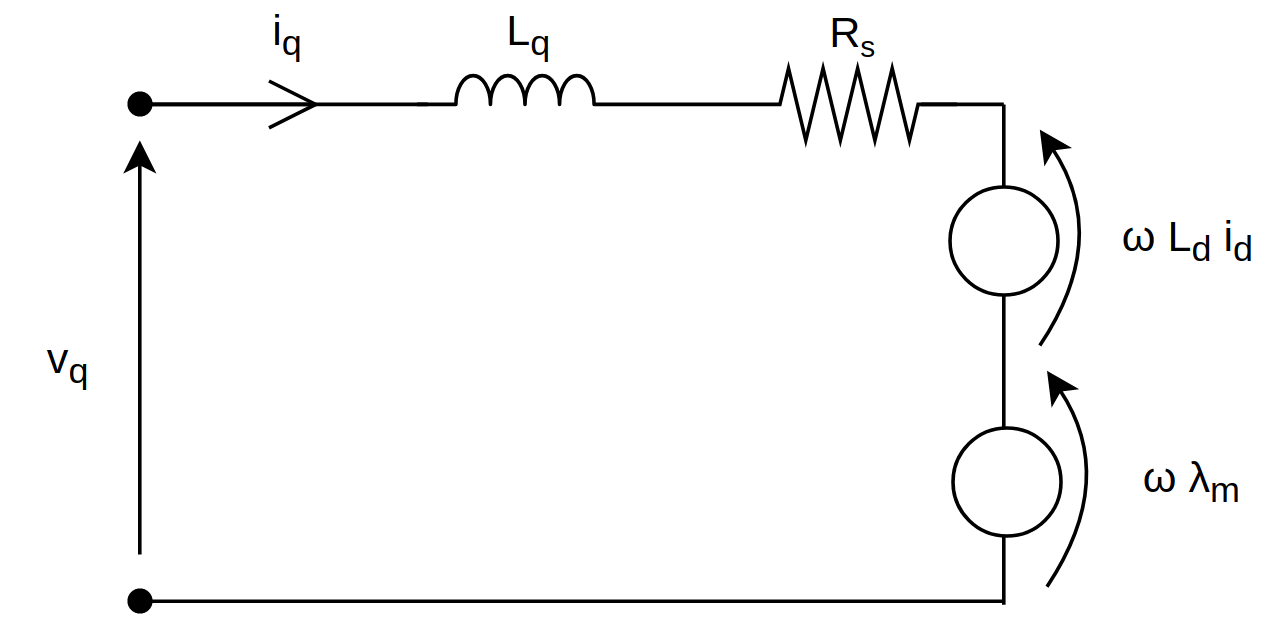
\includegraphics[width=0.6\linewidth]{pictures/control/vq.png}
	\caption{Q-direction equivalent circuit for the PMSM}
	\label{fig:vq}
\end{figure}

The voltage in the q-direction can be described from equation \ref{eq:q_direction}.

\begin{equation}
\label{eq:q_direction}
    v_q = L_q\frac{d i_q}{dt} + R_s i_q + \omega L_d i_d + \omega \lambda_m
\end{equation}

% \begin{equation}\label{eq:q_direction2}
% v_{sq} = R_si_q + \frac{d \varphi_{rd}}{dt} +  \omega_e \varphi_{rd}
% \end{equation}
% Where \\
% $\varphi_{rd} = L_di_d$

$\lambda_m$ is the flux linkage.

The $i_q$ from the $L_q \frac{di_q}{dt}$ part is isolated and Laplace transformed. This results in equation \ref{eq:d_direction}.

\begin{equation}
    \label{eq:q_direction2}
    I_q = \frac{1}{S} \frac{1}{L_q} (V_q - I_q R_q - \omega L_d I_d - \omega \lambda_m)
\end{equation}

From equation \ref{eq:q_direction2} the q-direction model can be produced. The model can be seen on figure \ref{fig:simulink_q_direction}.

\begin{figure}[H]
	\centering
	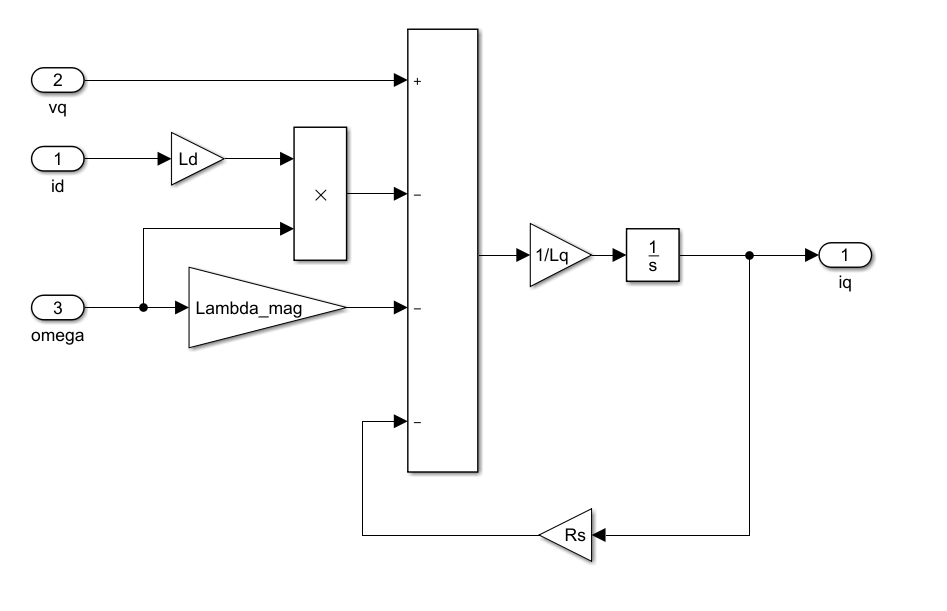
\includegraphics[width=0.8\linewidth]{pictures/control/simulink_q_direction.PNG}
	\caption{Simulink model of the q-direction of the motor model}
	\label{fig:simulink_q_direction}
\end{figure}


\subsubsection{Mechanical model}
For a multiple pole synchronous motor, the torque produced from the electrical field can be found from equation \ref{eq:torque_equation}.

\begin{equation}
    \label{eq:torque_equation}
    T_e = \frac{3P}{2} \big(\lambda_m i_{q} + (L_d - L_q) i_q i_{d}\big)
\end{equation}

Where $P$ is the number of pole pairs.

Because $L_q$ is higher than $L_d$, it can be seen from equation \ref{eq:torque_equation} the current running in the d-direction produces negative torque and is therefore reducing the output torque. 

The total torque at shaft of the motor, will be the sum of the torque the electrical field produces, the torque produces by the friction in the motor, and a possible external load torque. The total torque can be set equal to the inertia of the system multiplied with the acceleration. As seen in equation \ref{eq:total_torque}.

\begin{equation}
    \label{eq:total_torque}
    J\frac{d\omega}{dt} = T_e - B\omega - T_{load}
\end{equation}

$J$ is the inertia, $B$ is the friction coefficient, and $T_{load}$ is the torque from the external load.
Equation \ref{eq:total_torque} is rewritten and combined with equation \ref{eq:torque_equation} to a equation for the rotational speed. This is Laplace transformed, and the result is equation \ref{eq:omega}.

\begin{equation}
    \label{eq:omega}
    \omega = \frac{1}{S} \frac{1}{J} \bigg( \frac{3P}{2} \big( \lambda_m I_q + (L_d - L_q) I_q I_d \big) - B\omega - T_{load} \bigg)
\end{equation}

From equation \ref{eq:omega} can a model with the torque, rotational speed, and the angle of the motor as output, and the d- and q-current as inputs. This model can be seen on figure \ref{fig:torque}.

\begin{figure}[H]
	\centering
	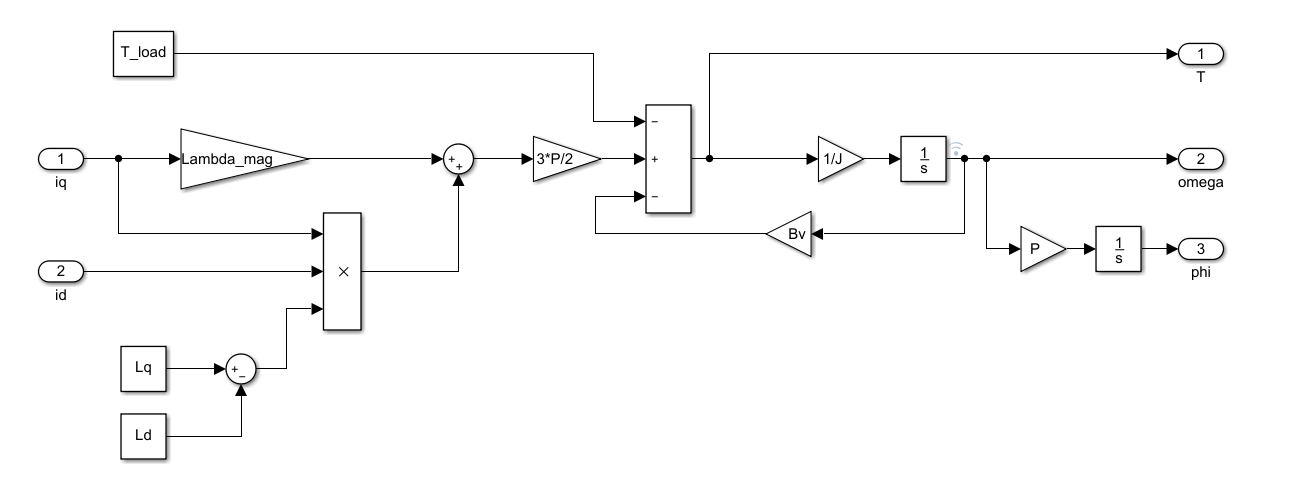
\includegraphics[width=1\linewidth]{pictures/control/torque.PNG}
	\caption{Simulink model of the motor with torque, rotational speed and the position of the rotor as output and the the d- and q-current as input}
	\label{fig:torque}
\end{figure}

\subsubsection{Complete motor model}
The three models, for the d-direction, the q-direction and the mechanical part, are put into subsystems and connected. This can be seen on figure \ref{fig:motor}

\begin{figure}[H]
	\centering
	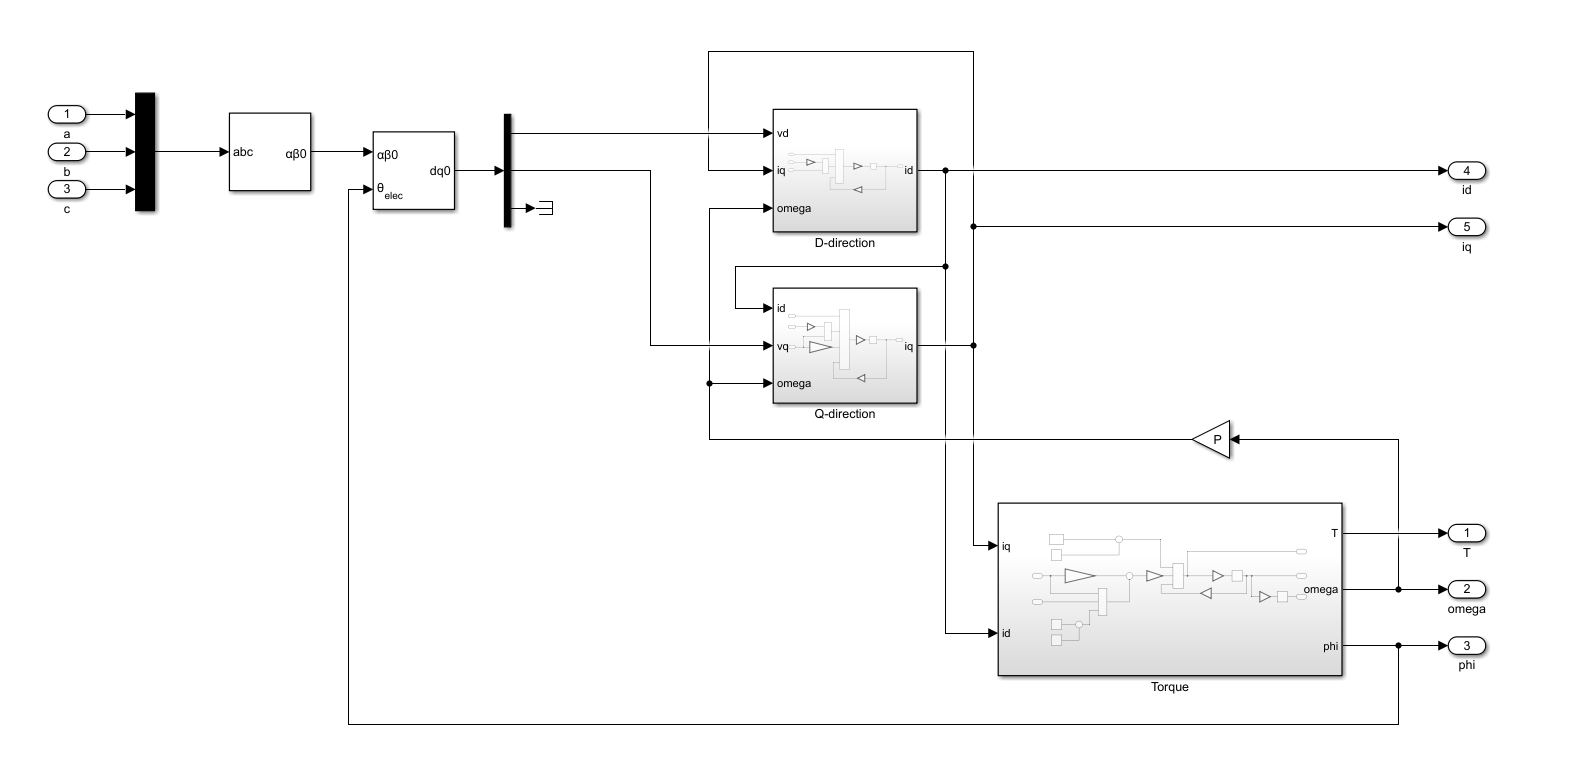
\includegraphics[width=1\linewidth]{pictures/control/motor_model.PNG}
	\caption{Simulink model of the full motor model}
	\label{fig:motor}
\end{figure}

Because the motor model is in the dq-frame, the three rotational phases voltages is converted to the dq-frame in the beginning of the model. The model outputs the d- and q-current, the torque, speed and angle of the motor. The rotational speed outputted from the motor model is the mechanical speed, and is therefore converted to the electrical speed before it is inputted to the d- and q-models. 



\subsection{Control system}
\label{sec:control_system}

For controlling the motor, the output d- and q-current of the motor are feedback to a PI-controller for each of them. The d-current is desired to be zero, and is therefore compared with zero before the PI-controller. The q-current is desired to be set to the reference point set by the input from the torque pedal. The torque reference input is therefore converted to a current, which can be compared with the feedback q-current from the motor model.

After the PI-controller the d- and q-voltages are converted back into three phases with an Inverse Clarke and an Inverse Park transformation. The three phase voltages are then put into the motor model.

The full model of the system can be seen on figure \ref{fig:control_system}.


\begin{figure}[H]
	\centering
	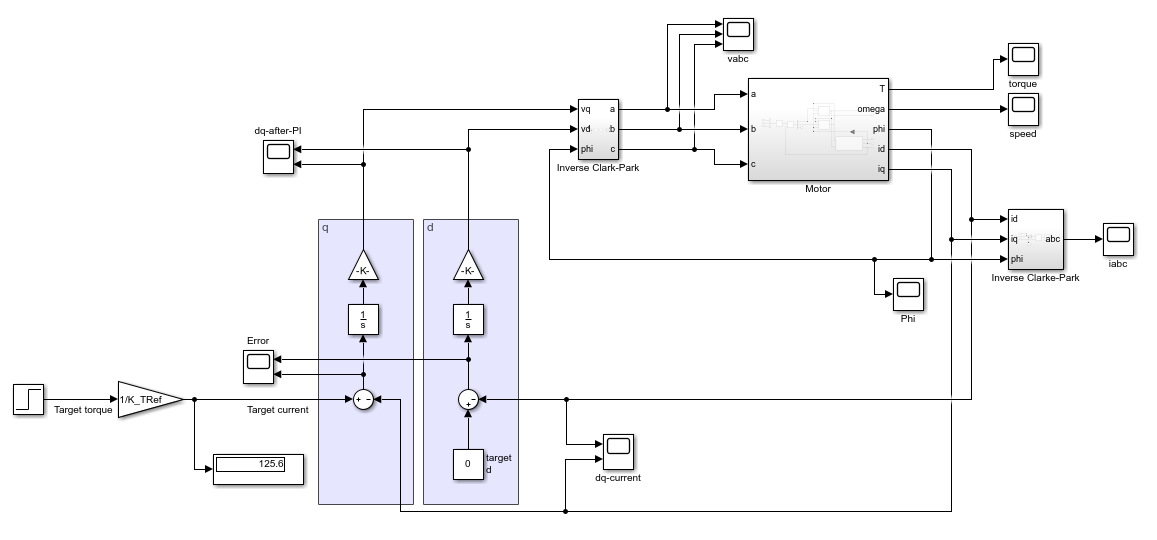
\includegraphics[width=1\linewidth]{pictures/control/full_model.PNG}
	\caption{The entire control model, with PI controller and motor model.}
	\label{fig:control_system}
\end{figure}



\subsection{PI-controller}

To set the PI-controller the transfer functions for the d- and q-direction is determined, with the voltages as input and the current as output. This is done based on the equations for the voltages in the d- and q-direction, equation \ref{eq:d_direction} and \ref{eq:q_direction}.
Because a transfer function only can have one input and one output, the two equation, \ref{eq:d_direction} and \ref{eq:q_direction}, is shortened. The new equation can be seen in equation \ref{eq:d_direction3} and \ref{eq:q_direction3}.

\begin{equation}
    \label{eq:d_direction3}
    v_d = L_d \frac{d i_d}{dt} + R_s i_d
\end{equation}

\begin{equation}
    \label{eq:q_direction3}
    v_q = L_q \frac{d i_q}{dt} + R_s i_q
\end{equation}

As seen in the two equations, \ref{eq:d_direction3} and \ref{eq:q_direction3}, the parts in the equations depending on other variables than the current is neglected. 
This Laplace transformed and converted to the transfer functions for the two systems.

\begin{equation}
    \frac{I_d(s)}{V_d(s)} = \frac{ \frac{1}{ \frac{L_d}{R_s} } }{ \frac{R_s}{ \frac{L_d}{R_s} } + R_s s }
\end{equation}

\subsection{Simulation}
\label{sec:simulation}
The model is tested with a step from $0$ to $47.8 Nm$, which correspond to a target q-current of $300 A $. At the start the load torque is set to $20 Nm$, and after $0.5 s$ it is increased to $40 Nm$. 

The three phase currents produced can be seen on figure \ref{fig:iabc}.

\begin{figure}[H]
	\centering
	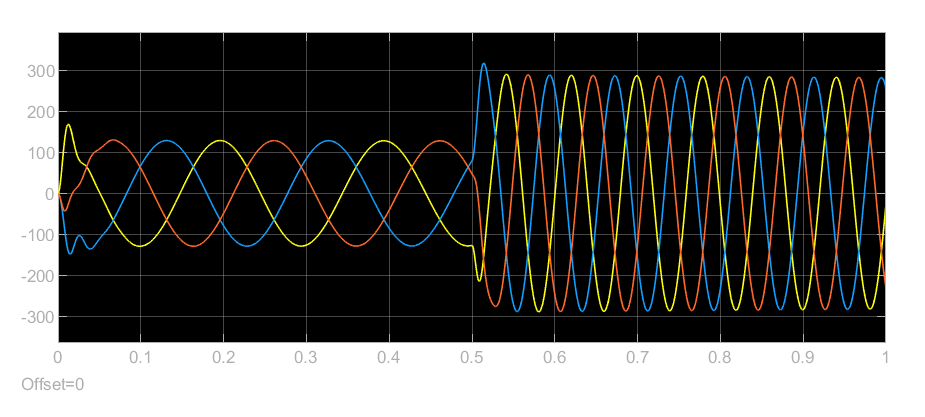
\includegraphics[width=0.6\linewidth]{pictures/control/iabc.eps}
	\caption{The ABC current from the motor model}
	\label{fig:iabc}
\end{figure}

As it it seen in figure \ref{fig:iabc}, the amplitude of the current increases when a bigger load is put on the motor. 
% A higher demand of current was expected when a bigger load is put on the motor. 

The d- and q-current can be seen on figure \ref{fig:idq}.

\begin{figure}[H]
	\centering
	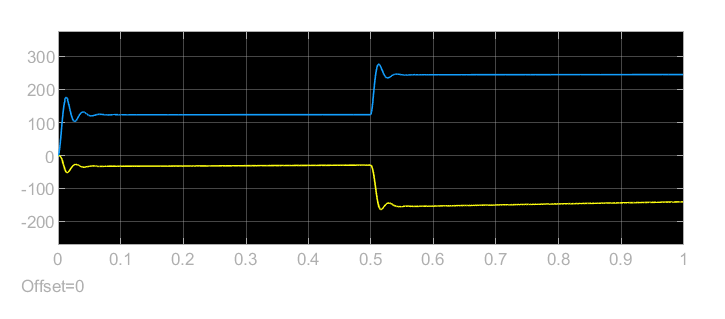
\includegraphics[width=0.6\linewidth]{pictures/control/idq.eps}
	\caption{The d- and q-current from the motor model. The yellow curve is the d-current and the blue curve is the q-current}
	\label{fig:idq}
\end{figure}

On figure \ref{fig:idq} it can be seen that the q-current is not going toward the set reference. It can also be seen that the d-current is very slowly going towards zero.

On the figure \ref{fig:speed} and \ref{fig:torque} the speed and the torque of the motor can be seen.

\begin{figure}[H]
	\centering
	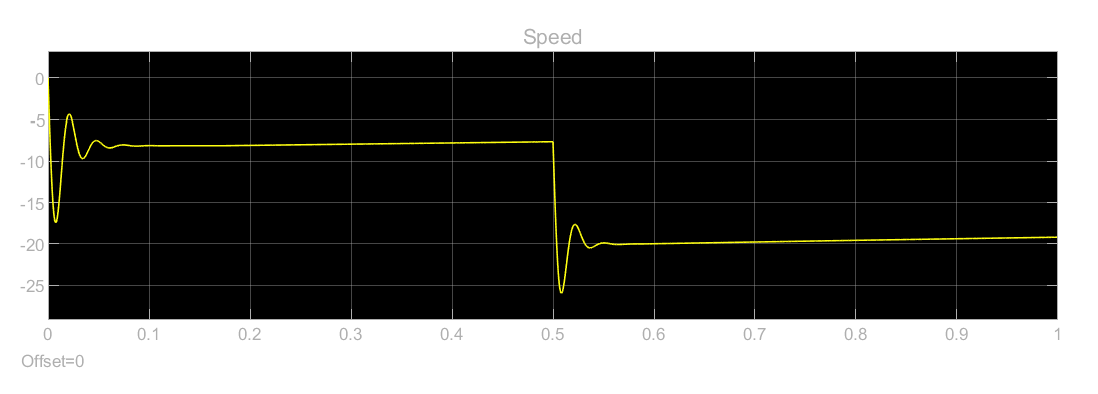
\includegraphics[width=0.7\linewidth]{pictures/control/speed.eps}
	\caption{The speed of the motor}
	\label{fig:speed}
\end{figure}

\begin{figure}[H]
	\centering
	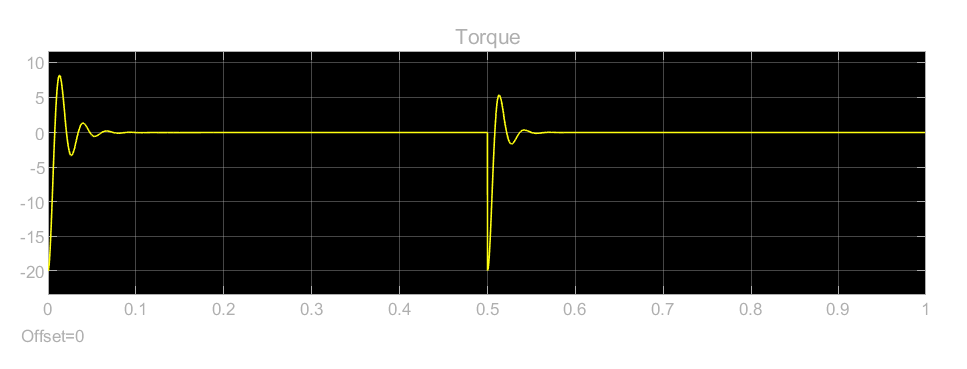
\includegraphics[width=0.7\linewidth]{pictures/control/torque.eps}
	\caption{The torque of the motor}
	\label{fig:torque}
\end{figure}



\subsection*{Subconclusion}


\newpage
% Software

\section{Embedded system}
\label{sec:embedded_system}
The embedded system's task is to handle the control for the inverter.

The section is divided into three subsections. First the overall system architecture, then the low-level drivers implemented in the FPGA part of the controller and lastly the processing system and interface with a computer. 




% Software structure
\subsection{Software structure}
The control is implemented on a Xilinx Zybo board which is a controller consisting of a FPGA part and a dual-core ARM Cortex-A9 processor.

Low-level drivers are implemented in the logic to allow the modules to run in parallel. The field orientated control as well as the interface to a PC is implemented on the processor which gives the possibility to have a higher abstraction. 

An overview of the system can be seen on figure \ref{fig:embedded_overview}. In the top is the processing system (PS) with an Interrupt Service Routine (ISR) and the control loop. The control loop outputs its result into a piece of block RAM from where the programmable logic (PL) can access it. The processing system also manages the interface to the PC which is done through UART.

\begin{figure}[H]
	\centering
	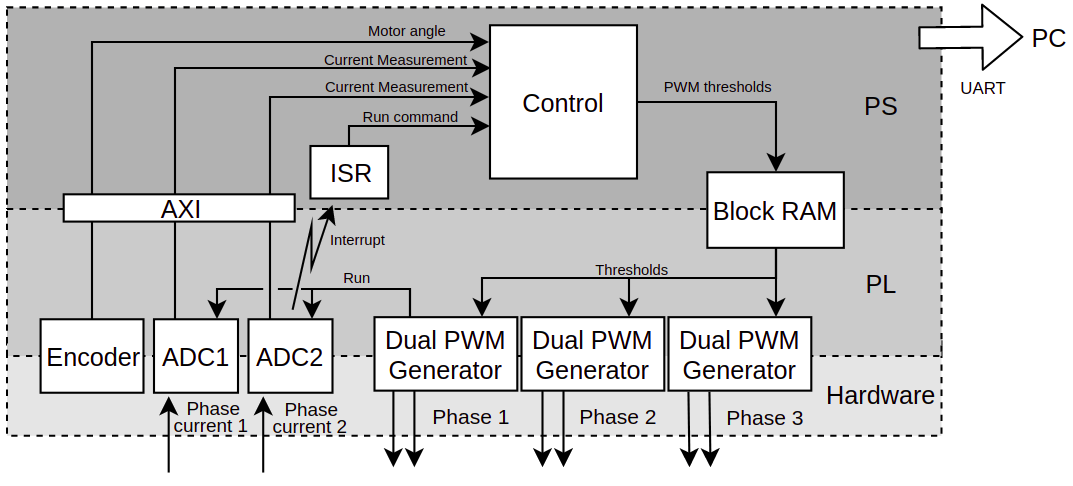
\includegraphics[width=1\linewidth]{pictures/software/embedded_overview.png}
	\caption{Embedded system overview}
	\label{fig:embedded_overview}
\end{figure}


In the programmable logic the drivers for three dual PWM generator are implemented. Each PWM generator control one phase in the inverter. The PWM generators all generate a pulse in the middle of their PWM periods. One of these are parsed to the ADC's and used to trigger a reading of the phase currents and the torque pedal. When the ADC's are done converting all inputs they produce an interrupt that triggers the ISR in the processing system.

The ADC readings as well as the encoder readings are parsed to the processing system through the AXI interface.



On figure \ref{fig:software_flow} the flowchart of the control loop implemented on the processing system can be seen. The system is waiting to receive the run command from the ISR which is triggered once every PWM period, see section \ref{sec:isr} for more about the ISR. 


\begin{figure}[H]
	\centering
	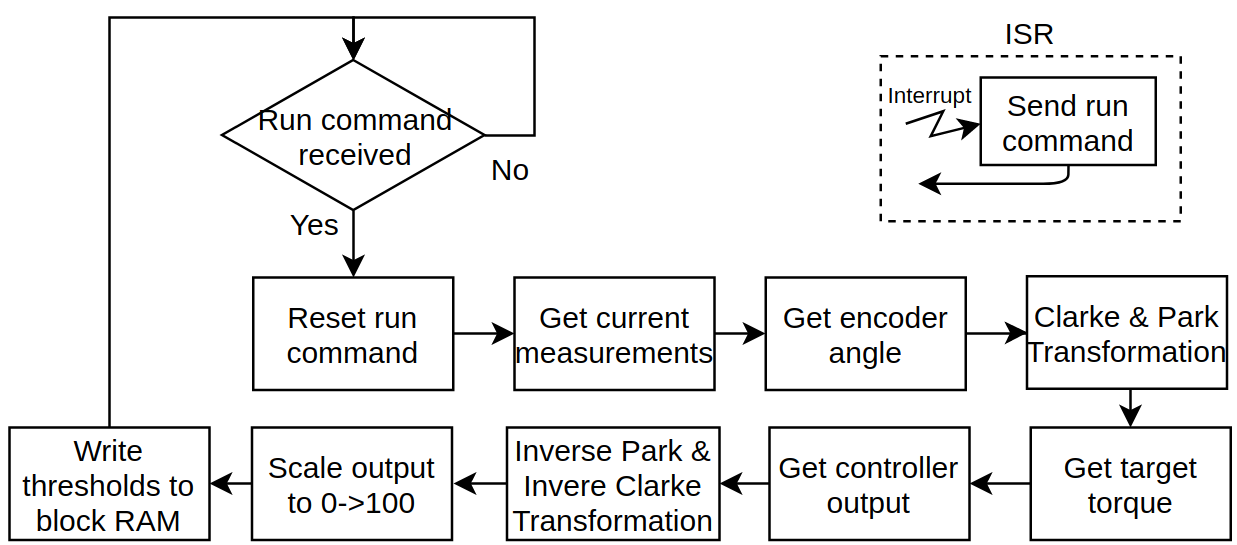
\includegraphics[width=0.9\linewidth]{pictures/software/software_flow.png}
	\caption{Processing System Overview}
	\label{fig:software_flow}
\end{figure}

When the run command is received it is first reset to get ready for the next command. Then the current measurements from the two ADC's are read into the system as well as the rotor angle from the encoder. A Clarke and a Park transformation is performed. The torque pedal position is read and the two PI controllers as discussed in section \ref{sec:control_system} perform the control. The result from the controllers are then transformed with an Inverse Park and an Inverse Clarke Transformation which produces three control signals. These signals are then linearly mapped to the range $0 \rightarrow 100$, which is what the PWM generators are compatible with. 
The thresholds are then written to a piece of block RAM shared between the PS and the PL. The PS will then wait for the next run command.





%%%%%%%%%%%%%%%%%%%%% PL %%%%%%%%%%%%%%%%%%%%%
\subsection{Programmable Logic (PL)}
To take advantage of the parallel and super fast nature of FPGA logic all the low-level drivers are placed in logic. The section will go through the development and use of the modules used which includes a PWM module, an encoder module and an ADC module.

% PWM generator
\subsubsection{PWM module}
\label{sec:pwm}
Each phase of the inverter is controlled by a PWM signal for the high-side and low-side of each leg.

The module shown on figure \ref{fig:pwm_module} is made to control a whole leg. Three instances of the module can be used to control all three phases.
\begin{figure}[H]
	\centering
	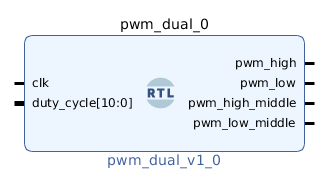
\includegraphics[width=0.5 \textwidth]{pictures/software/pwm_module.png}
	\caption{The PWM module made to control both high-side and low-side transistors of a leg in the inverter.}
	\label{fig:pwm_module}
\end{figure}
The module takes in a clock signal and a target duty cycle. The module then output two PWM signals inverse of each other and two pulse signals each sending out a pulse in the middle of their respective PWM signal.


\subsubsection*{Counter}
A counter is used for implementing the PWM. For every rising edge of the input clock the counter takes one step up or down depending on its current counting direction. When it reaches one of its outer limits the counting direction is switched as can be seen on figure \ref{fig:counter}.

\begin{figure}[H]
	\centering
	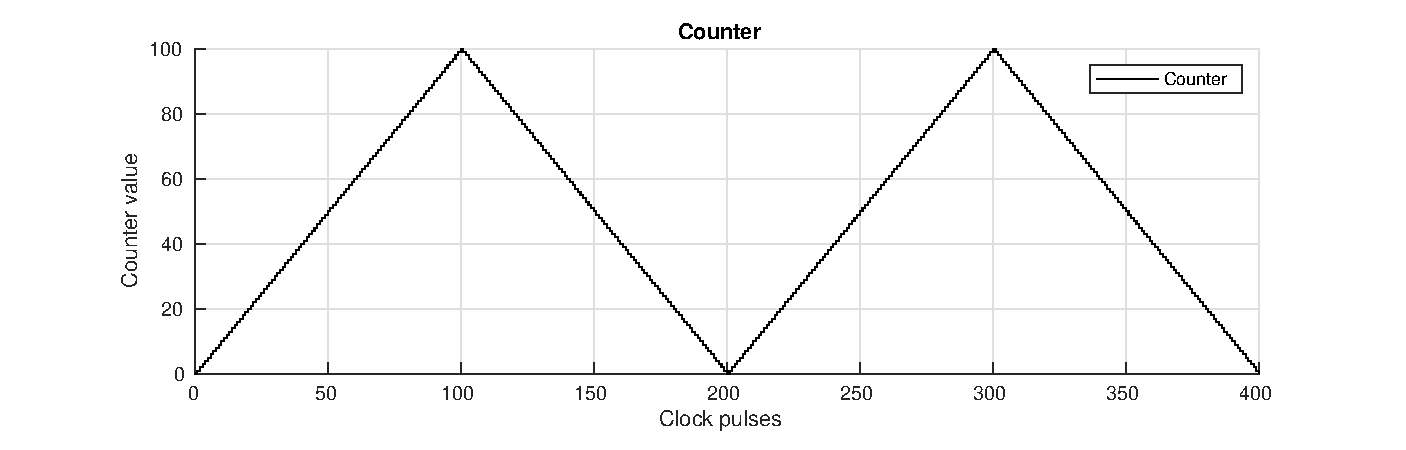
\includegraphics[width=1 \textwidth]{pictures/software/counter.eps}
	\caption{How the counter is counted up and down over time.}
	\label{fig:counter}
\end{figure}

The resolution of the PWM duty cycle is chosen to be $1\%$ which means the counter takes $100$ steps from minimum to maximum. The PWM is made as a phase correct PWM which means it will have the same phase no matter the duty cycle. Therefore the counter counts both up and down per period which results in $200$ steps per period. 

The signal out of the PWM generator should be the same frequency as the inverter components are designed for in the earlier sections which is $10kHz$. The input clock is already prescaling the output frequency by the number of counter steps but this is not enough and therefore in order for the PWM to have the correct frequency an additional prescaler is added. The prescaler value is found with equation \ref{eq:additional_prescaler}.

The prescaler is constructed with a counter counting up a value, $x$. When the value is reached the output clock is flipped and the counter is reset. Such a prescaler has a build in prescaling of 2 which is added besides the additional prescaler leading to equation \ref{eq:additional_prescaler1}.



\begin{subequations}
    \begin{align}
        \begin{split}
            f_{s} = \frac{f_{pl}}{c_{steps} \cdot x \cdot 2}
            \label{eq:additional_prescaler1}
        \end{split} \\ 
        \begin{split}
             x = \frac{f_{pl}}{f_{s} \cdot c_{steps} \cdot 2}
        \end{split} \\ 
        \begin{split}
            x = \frac{125MHz}{10kHz \cdot 200 \cdot 2} = 31.25 \sim 31
            \label{eq:additional_prescaler}
        \end{split} \\
        \begin{split}
            \frac{125MHz}{200 \cdot 31 \cdot 2} = 10.08kHz
        \end{split}
    \end{align}
\end{subequations}

Where $f_{s}$ is the output frequency of the PWM signal, $c_{steps}$ is the number of counter steps in a period, $f_{pl}$ is the logic clock which is $125MHz$ and $x$ is the additional prescaler.

With the additional prescaler the PWM module outputs PWM signals with a frequency of $10.08kHz$.

\subsubsection*{PWM}


To handle both a high-side PWM and low-side PWM each of the signals have a threshold and the output signal changes from high to low or opposite when the counter crosses the threshold as can be seen in figure \ref{fig:counter_with_pwm}. The two thresholds are spaced out with a static deadtime between them which is discussed later in this section. The deadtime on figure \ref{fig:counter_with_pwm} has been exaggerated to make it more visible.

\begin{figure}[H]
	\centering
	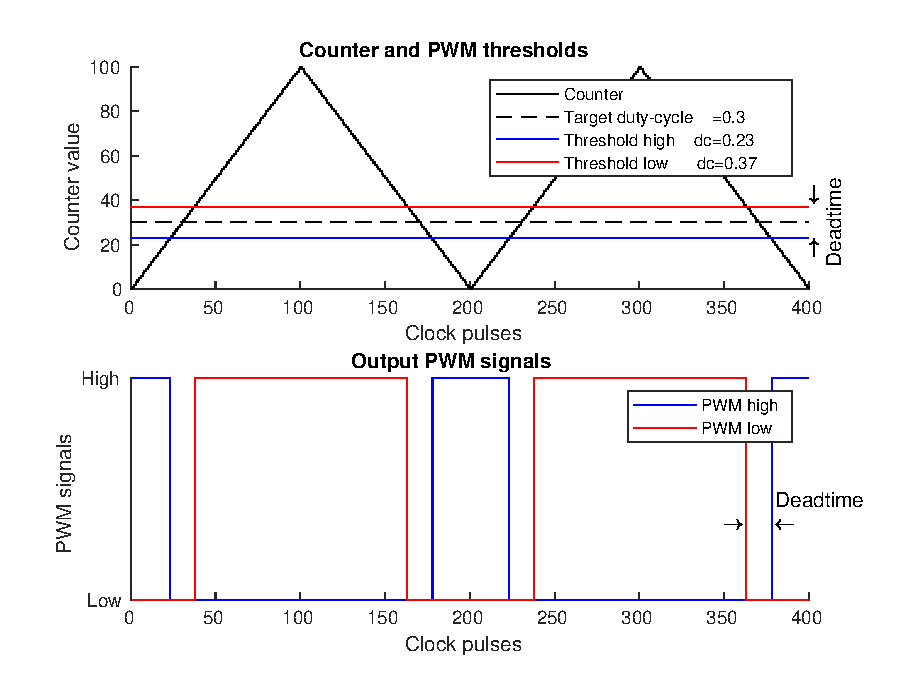
\includegraphics[width=0.85 \textwidth]{pictures/software/counter_with_pwm.eps}
	\caption{The top shows the target duty-cycle together with the thresholds compared to the PWM counter. The bottom shows the output PWM signals. The deadtime is exaggerated to make it more visible.}
	\label{fig:counter_with_pwm}
\end{figure}

The high-side PWM is high when the counter is below the high-side threshold, $counter < th_{high}$, otherwise it is low. 

The low-side PWM is high when the counter is above the low-side threshold, $counter > th_{low}$ otherwise it is low.

The VHDL code can be seen below.

\begin{minted}[frame=single,framesep=2mm,baselinestretch=1.2,linenos,fontsize=\footnotesize]{vhdl}
-- Control of the high side PWM
pwm_high <= HIGH when (counter < threshold_high) else LOW;
-- Control of the low side PWM
pwm_low  <= HIGH when (counter > threshold_low) else LOW;
\end{minted}
\begin{center}
    The VHDL code to control the PWM signals.
\end{center}


To avoid shorting the supply deadtime is inserted between turning off one transistor and turning on the other.

On figure \ref{fig:turn_off_time1} the conducted current for each transistor is drawn next to the PWM signals with deadtime being bigger than the transistor turn off time, $dead \ time > t_{turn \ off}$, which results in one transistor turning completely off before the other turns on. 

\begin{figure}[H]
	\centering
	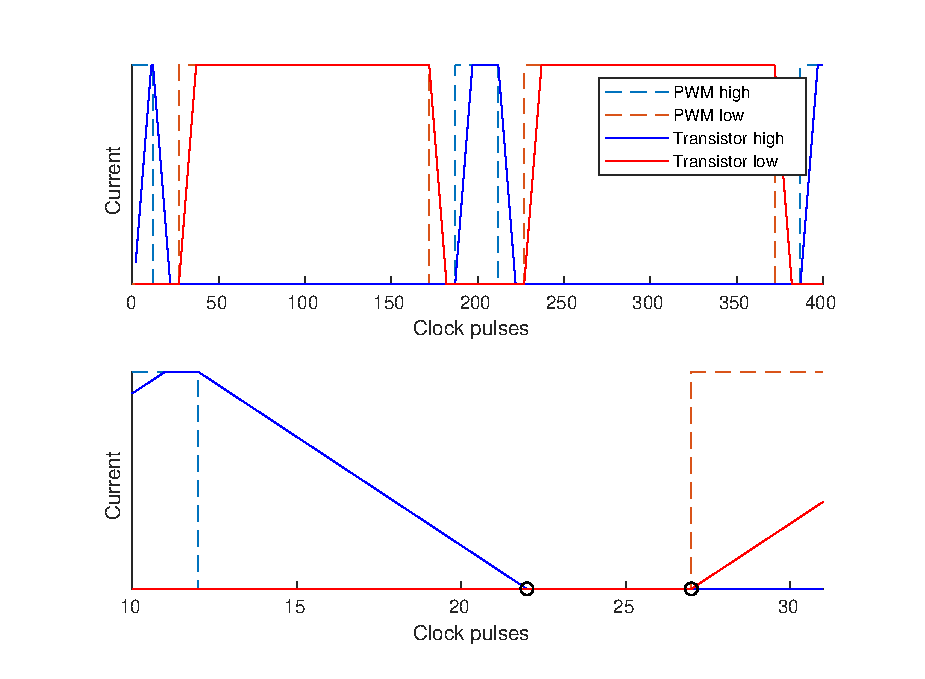
\includegraphics[width=0.8 \textwidth]{pictures/software/turn_off_time1.eps}
	\caption{PWM with deadtime and transistor conduction curves for systems with $dead \ time > t_{turn \ off}$}
	\label{fig:turn_off_time1}
\end{figure}

On figure \ref{fig:turn_off_time2} the conducted current for each transistor is drawn next to the PWM signals but this time the deadtime is smaller than the transistor turn off time, $dead \ time < t_{turn \ off}$, which results in both transistors conducting at the same time.
When both transistors conduct the supply is shorted which should be avoided especially when the supply consist of batteries.

\begin{figure}[H]
	\centering
	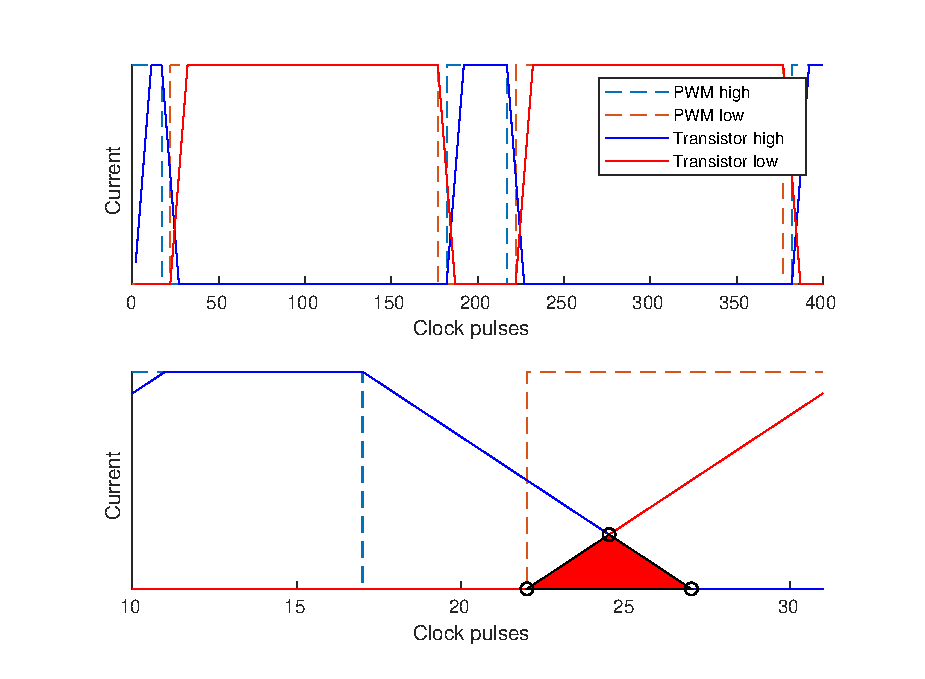
\includegraphics[width=0.8 \textwidth]{pictures/software/turn_off_time2.eps}
	\caption{PWM with deadtime and transistor conduction curves for systems with $dead \ time < t_{turn \ off}$}
	\label{fig:turn_off_time2}
\end{figure}

It is therefore important to choose the deadtime big enough to avoid shorting but also not so big that the systems performance is unnecessarily reduced.
\bigskip


To avoid compromising the required deadtime at edge cases where one of the thresholds tries to move above $100 \%$ or  below $0 \%$ the thresholds are found in two different ways.





When the high-side threshold is greater than the counter minimum plus half of the deadtime it is placed half of the deadtime below the threshold.
\begin{equation}
    th_{duty \ cycle} \geq  c_{min} + \frac{t_{dead \ time}}{2}
    \label{eq:threshold_high_condition}
\end{equation}
\begin{center}
    $\Downarrow$    
\end{center}
\begin{equation}
   th_{high} = th_{duty \ cycle} - \frac{t_{dead \ time}}{2}  
   \label{eq:threshold_high_equation}
\end{equation}

Otherwise the threshold is clamped to the counter bottom edge $th_{high} = counter_{min}$ which is possible because the PWM is switched when $th_{high} > counter$.
If the threshold comes too close to the edge the threshold will be clamped and the PWM will not switch. Had the PWM being switched when $th_{high} \geq counter$ this would not have worked.



The low-side threshold is placed half of the deadtime above the threshold when the duty cycle is at least half of the deadtime below the counter max.
\begin{equation}
    th_{duty \ cycle}\leq c_{max} - \frac{t_{dead \ time}}{2}
    \label{eq:threshold_low_condition}
\end{equation}
\begin{center}
    $\Downarrow$
\end{center}
\begin{equation}
  th_{low} = th_{duty \ cycle} + \frac{t_{dead \ time}}{2}  
  \label{eq:threshold_low_equation}
\end{equation}
Otherwise the threshold is clamped to the top counter edge.

The VHDL code to find the two thresholds can be seen below. The variable \textit{duty\textunderscore cycle} is parsed into the PWM module. \textit{DEADTIME}, \textit{HALF\textunderscore DEADTIME}, \textit{COUNT\textunderscore MIN} and \textit{COUNT\textunderscore MAX} are all constants.

\begin{minted}[frame=single,framesep=2mm,baselinestretch=1.2,linenos,fontsize=\footnotesize]{vhdl}
-- Get half of deadtime
HALF_DEADTIME(6 downto 0) <= DEADTIME(7 downto 1);
-- Find the threshold for the high-side PWM
threshold_high <= duty_cycle - HALF_DEADTIME when 
                (duty_cycle >= COUNT_MIN + HALF_DEADTIME) else COUNT_MIN;
-- Find the threshold for the low-side PWM
threshold_low  <= duty_cycle + HALF_DEADTIME when 
                (duty_cycle <= COUNT_MAX - HALF_DEADTIME) else COUNT_MAX;
\end{minted}
\begin{center}
    The VHDL code to find the thresholds for the high and low side PWM signals. The conditions and equations used are \ref{eq:threshold_high_condition}, \ref{eq:threshold_high_equation}, \ref{eq:threshold_low_condition} and \ref{eq:threshold_low_equation}.
\end{center}



The turn off times for the transistors was found in section \ref{sec:switching_power_loss} to be $75ns$.
The way deadtime is implemented it has to be defined as some even amount of ticks at the PWM frequency.
The minimum deadtime step, $dt_{res}$, in this system is calculated with equation \ref{eq:minimum_deadtime_resolution}.

\begin{subequations}
    \begin{align}
        \begin{split}
            dt_{res} = \frac{T}{2} \cdot \frac{dt_{min}}{c_{max}}
        \end{split} \\ 
        \begin{split}
             dt_{res} = \frac{2}{fs} \cdot \frac{dt_{min}}{c_{max}}
        \end{split} \\ 
        \begin{split}
             dt_{res} = \frac{2}{10kHz} \cdot \frac{2}{100} = 4\mu s
        \end{split} 
    \end{align}
    \label{eq:minimum_deadtime_resolution}
\end{subequations}

Which gives the system a safety margin of $\sim 53$ on the deadtime between the two PWM signals.


\subsubsection*{ADC Pulses}

To trigger a new reading by the ADC the PWM generator module has a build-in pulse mechanism that outputs a pulse in the middle of each of the PWM periods as can be seen on figure \ref{fig:adc_pulses}. Only the pulse in the middle of the high-side PWM is used to trigger the ADC. The reason for measuring in the middle of the PWM is to avoid majority of the ringing produced on the signals from switching.

\begin{figure}[H]
	\centering
	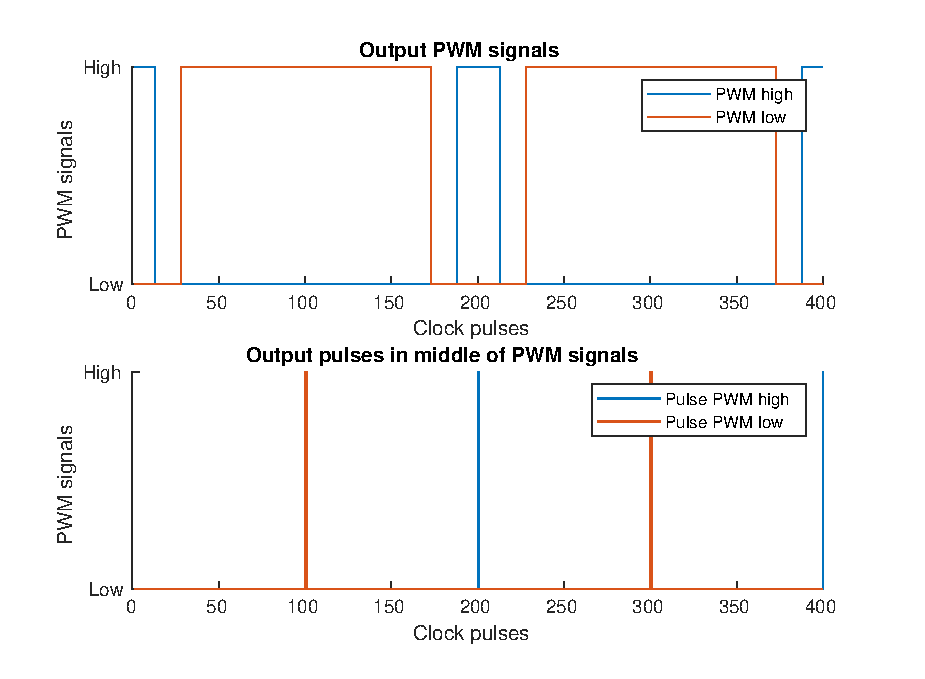
\includegraphics[width=0.8 \textwidth]{pictures/software/adc_pulses.eps}
	\caption{The top graph shows the high and low side PWM signals. The bottom graph shows the ADC pulses triggered in the middle of each PWM signal.}
	\label{fig:adc_pulses}
\end{figure}

The code for evaluating the signal states can be seen below. 
% The code utilizes the concurrent nature of VHDL which makes it fast and robust.
When the counter reaches its bottom edge the high pulse is set high and as soon as the counter starts going up again the signal is set low. The low pulse is controlled in the same way but this happens at the high counter edge instead.

\begin{minted}[frame=single,framesep=2mm,baselinestretch=1.2,linenos]{vhdl}
-- Output a pulse in the middle of the high PWM signal
pwm_high_middle <= HIGH when (counter <= COUNT_MIN) else LOW;

-- Output a pulse in the middle of the low PWM signal
pwm_low_middle <= HIGH when (counter >= COUNT_MAX) else LOW;
\end{minted}
\begin{center}
    The VHDL code to control the ADC pulses.
\end{center}


\subsubsection*{Test of PWM module}

To test the PWM generators a test scenario is set up. A simulated rotor angle and simulated currents are parsed into the control system and the outputs are measured with an oscilloscope. 
The maximum sine frequency expected out of the system is $333Hz$. To figure out how fast the simulated angle should change the time between each angle change is found. 
The angle is chosen to with $1$ degree steps. That gives a change rate of:


\begin{equation}
    change_{rate} = sin_{freq} \cdot 360^o
\end{equation}
Where $sin_{freq}$ is the target sine frequency. Which results in a time per angle of
\begin{equation}
    t_{angle} = \frac{1}{change_{rate}} = \frac{1}{333Hz \cdot 360^o} = 8 \mu s
\end{equation}
Where $t_{angle}$ is the time per angle. 

No currents will run in the system so the currents need to be simulate as well. The angle is used to calculate three sinusoidal curves. The way the three currents are calculated can be seen in equation \ref{eq:simulated_currents}.

\begin{equation}
    i_A = sin(angle), \ \ i_B = sin(angle + 120^o), \ \ i_C = sin(angle + 240^o)
    \label{eq:simulated_currents}
\end{equation}


Implementing this gives the PWM signal on one of the phases as seen in the top of figure \ref{fig:one_phase} and the resulting sine curve on the bottom.

\begin{figure}[H]
	\centering
	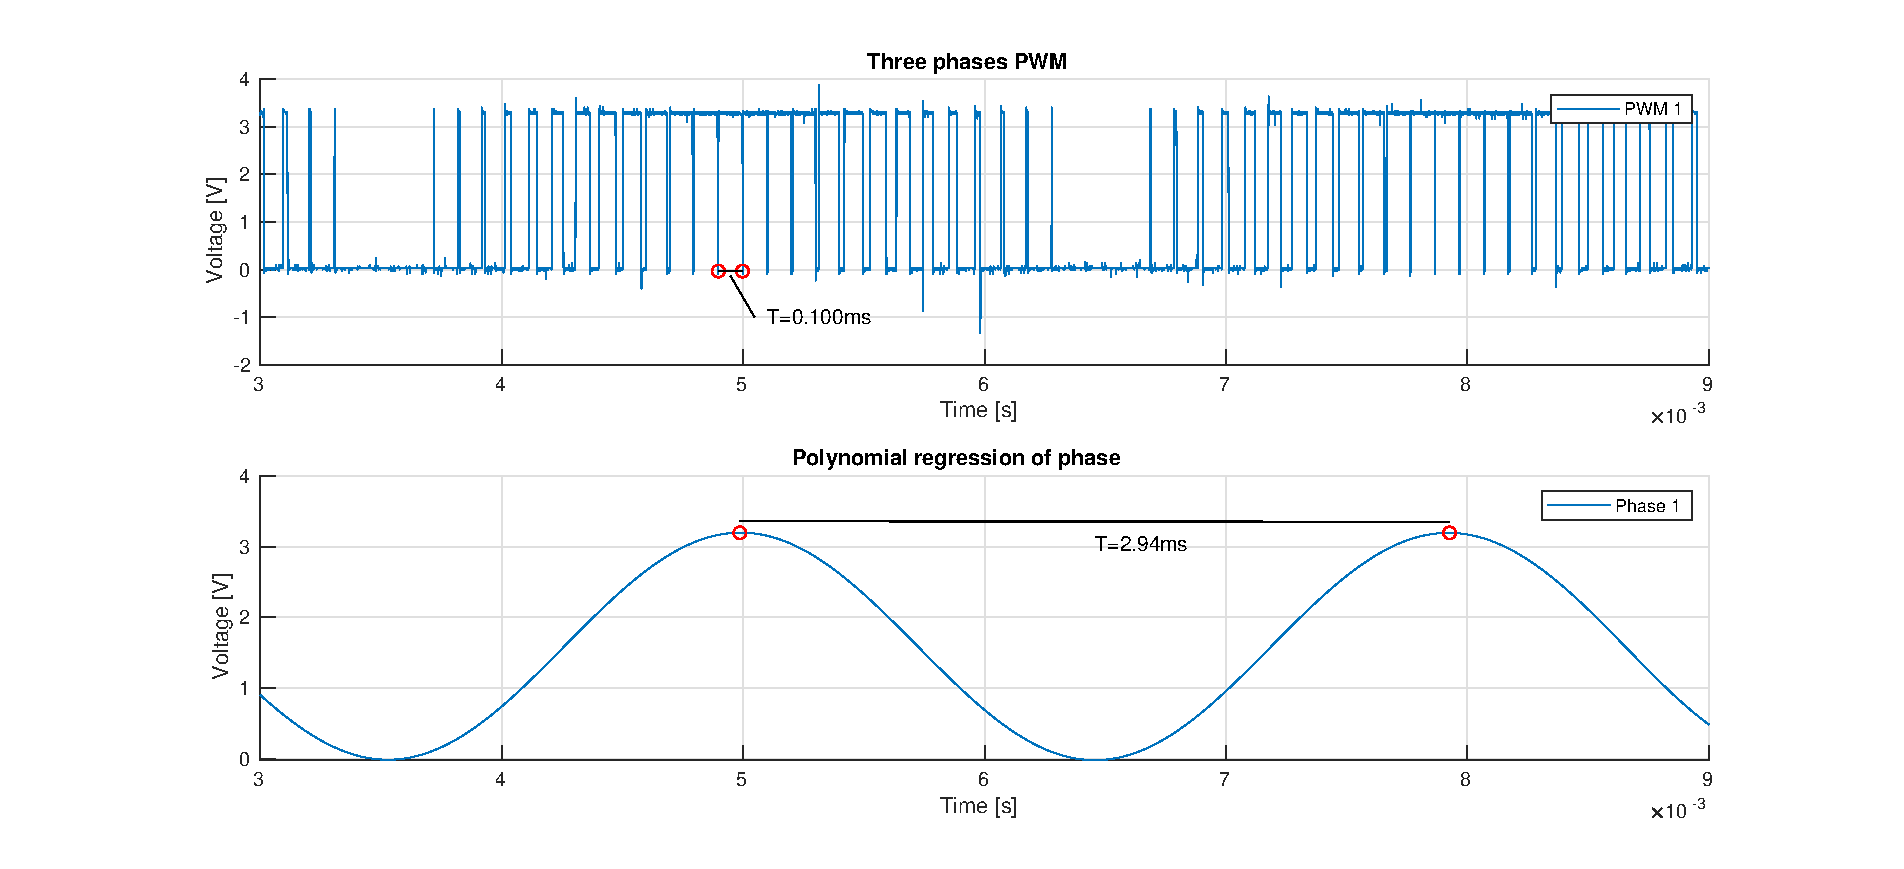
\includegraphics[width=1 \textwidth]{pictures/software/one_phase.eps}
	\caption{Testing of one phase. The top graph shows the PWM signals. The bottom graph shows the resulting sine curve found with a polynomial regression.}
	\label{fig:one_phase}
\end{figure}

The PWM frequency can be found by measuring the time between the middle of two PWM periods as can be seen in equation \ref{eq:pwm_frequency}. 
\begin{equation}
    f_s = \frac{1}{0.100 \cdot 10^{-3}} = 10kHz
    \label{eq:pwm_frequency}
\end{equation}
With a precision of 6 decimals on the time period the frequency of the PWM signal turns out to be $10kHz$.

The resulting sine can be found by applying a polynomial regression to the PWM signal which results in a sinusoidal curve. The frequency is found from the inverse of the time period between two points exactly one period apart. 
\begin{equation}
    sin_{freq} = \frac{1}{2.94 \cdot 10^{-3}} = 340 Hz
\end{equation}
The frequency of the sine is $340Hz$.

On figure \ref{fig:one_phase} only one of the phases are shown. In reality the system outputs three phases and all can be seen on figure \ref{fig:three_phases}. The periods in between the peak of the three phases are shown to determine the amount of phase shift. The time of one third of a period is calculated with \ref{eq:one_third_period}.
\begin{equation}
    \frac{1}{3} \cdot \frac{1}{340 Hz} = 0.9804ms
    \label{eq:one_third_period}
\end{equation}
By comparing the theoretical and measured periods between the phases it is determined that the phases are phase shifted with approximately $120^o = 2 \pi / 3 \ rad$.
\begin{figure}[H]
	\centering
	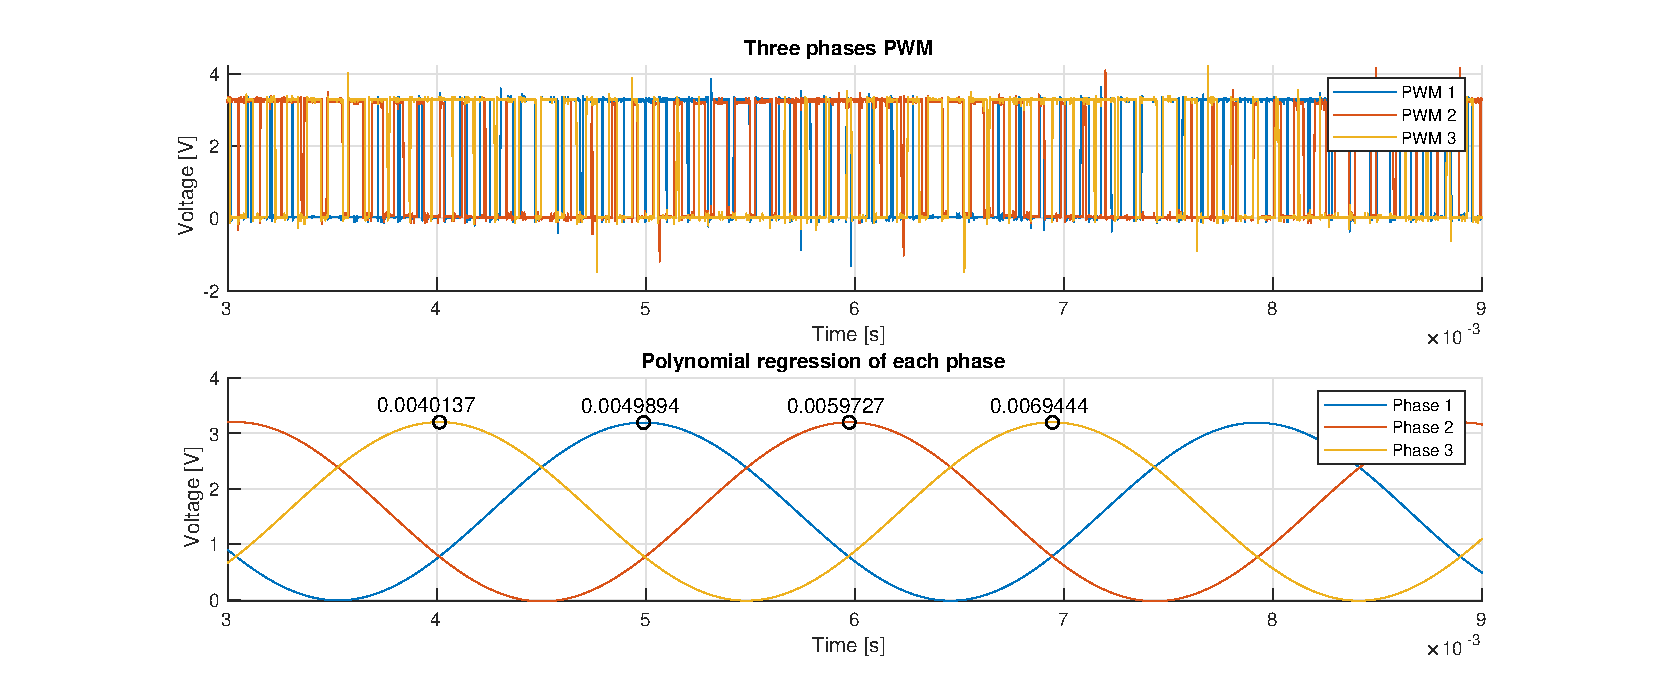
\includegraphics[width=1 \textwidth]{pictures/software/three_phases.eps}
	\caption{Testing of all three phases. The top graph shows the PWM signals. The bottom graph shows the resulting sine curves found with polynomial regressions.}
	\label{fig:three_phases}
\end{figure}


% Encoder
\subsubsection{Encoder}
\label{sec:encoder}

A driver module for the encoder on the motor was part of the material to get started on this project. \cite{encoder_module}

\begin{figure}[H]
	\centering
	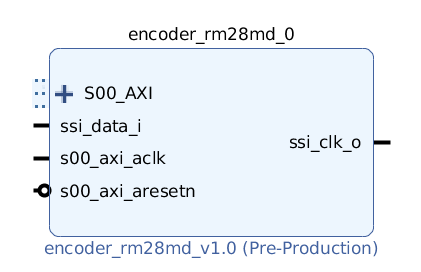
\includegraphics[width=0.4\textwidth]{pictures/software/encoder_module.png}
	\caption{The encoder driver module.}
	\label{fig:encoder_module}
\end{figure}
The driver module, as seen on figure \ref{fig:encoder_module}, supports an 8-bit encoder and takes care of handling the returned signal from the encoder itself. The module outputs the current rotor angle at a frequency determined by the PL clock and can be found with equation \ref{eq:encoder_frequency}.
\begin{equation}
f_{encoder} = \frac{f_{pl}}{6708} = \frac{125MHz}{6708} = 18.634kHz
\label{eq:encoder_frequency}
\end{equation}
The system runs at $10kHz$ which means the control loop will always have a new encoder angle at every cycle.


The encoder is a 8 bit encoder which means it has a resolution of $2^8 = 255$ steps per revolution. The motor has $4$ pole pairs which means the electric field inside the motor turns $4$ times each time the rotor turns $1$ time which means the resolution of the electric field angle is $1/4th$ of the mechanical rotor angle.
The two angles are both shown in figure \ref{fig:rotor_vs_electric_angle} where it can be seen that the electric angle moves 4 times faster than the rotor angle.

\begin{figure}[H]
	\centering
	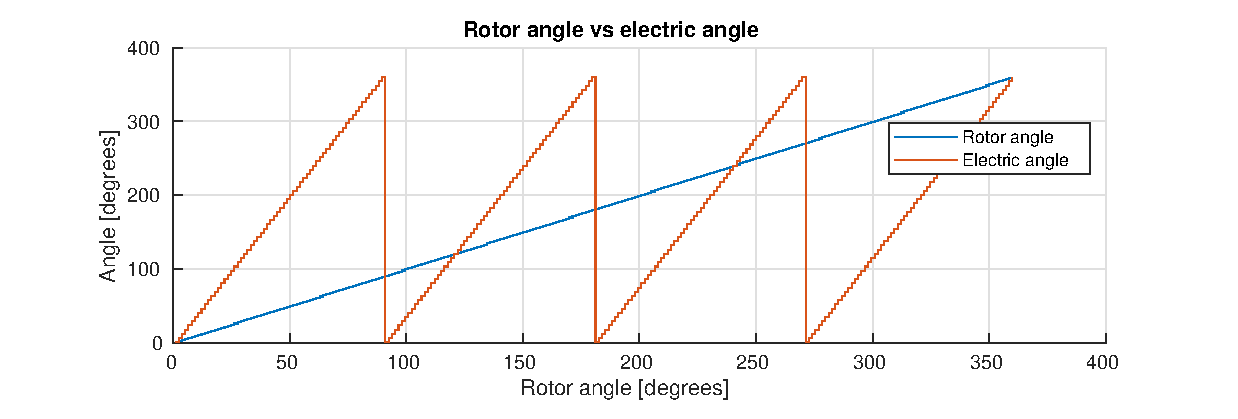
\includegraphics[width=1\textwidth]{pictures/software/rotor_vs_electric_angle.eps}
	\caption{Electric angle shown again the rotor angle.}
	\label{fig:rotor_vs_electric_angle}
\end{figure}

The resolution on the rotor angle and the electric angle can be calculated with equation \ref{eq:rotor_angle_error} and equation \ref{eq:electric_angle_error} respectfully. 

\begin{equation}
res_{rotor} = \frac{360^o}{2^8} = 1.412^o
\label{eq:rotor_angle_error}
\end{equation}

\begin{equation}
res_{electric} = \frac{360^o}{2^6} = 5.625^o
\label{eq:electric_angle_error}
\end{equation}




The rotor position is returned as an 8 bit value from the encoder module, and before the angle can be used in the control system it is first mapped from $0 \rightarrow 255$ to an actual angle going from $0^o \rightarrow 359^o$. The mapping is done with equation \ref{eq:angle_mapping}.
\begin{equation}
    angle = \frac{359}{255} \cdot position
    \label{eq:angle_mapping}
\end{equation}



\begin{lstlisting}[style=c, caption=Function to read an angle from the encoder. The angle is returned in degrees., label=code:encoder_angle_function]
f32 getRotorAngle(){
    u8 position = RM28MD_POSITION & 0x000000FF;     // Only the first byte is valid
    f32 angle   = 359/255 * position;       	      // Map position (0->255) to 
                                                    // angle (0->359)
    return angle;                                   // Return angle
}
\end{lstlisting}


\paragraph{Improve angle accuracy with linear interpolation}
\label{sec:linear_interpolation}
Low resolution and thereby big steps in the rotor angle results in uneven rotation of the motor especially at low speeds.
To improve the angle before it is used in the control the real angle is approximated with the use of linear interpolation. It is assumed that the rotor speed is approximately the same for each encoder value step. This assumption is not completely correct because it would mean the motor does not change speed. The rotor acceleration and deceleration is assumed slow enough compared to the encoder frequency to not result in big errors.


The formula for linear interpolation \cite{lin_interpol} can be seen in equation \ref{eq:linear_interpolation1}. 

\begin{equation}
    y = \Big( \frac{y_2-y_1}{x_2-x_1} \Big)(x-x_1)+y_1
    \label{eq:linear_interpolation1}
\end{equation}
Figure \ref{fig:angle_interpolation1} shows the scenario where the real angle, at point $p_2$, can be found from the measured angle, $p_1$, if $x_1$,$x_2$,$y_1$ and $y_2$ are known.
The equation can be converted to fit the system by setting the two $y$ values equal to the amount of change between the current and last step $\Delta a = y_2 - y_1$ and setting the $x$ values to be the step width $x_{step} = x_2 - x_1$. Assuming that the speed is approximately the same for the current step as it was on the last. Which results in equation \ref{eq:linear_interpolation2}.

\begin{equation}
    y =  \frac{\Delta a}{x_{step}} \Delta x+y_1
    \label{eq:linear_interpolation2}
\end{equation}

\begin{figure}[H]
	\centering
	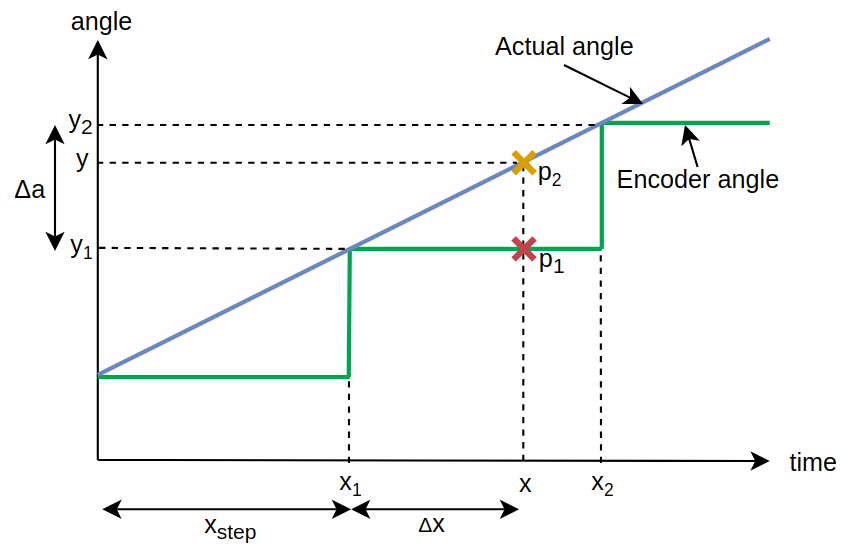
\includegraphics[width=0.8\textwidth]{pictures/software/angle_interpolation1.png}
	\caption{Ideal linear interpolation.}
	\label{fig:angle_interpolation1}
\end{figure}

The x-axis is discrete time and will be kept track of in relation to the number of samples passing and therefore $x$ will be denoted $n$. To know how fast the encoder values change over time this frequency is calculated with equation \ref{eq:encoder_step_frequency}.

\begin{equation}
    f = \frac{v_{[^o/s]}}{res_{rotor}} = 5000 [RPM] \cdot 6 \cdot \frac{360^o}{2^8} = 42188Hz
    \label{eq:encoder_step_frequency}
\end{equation}

The frequency is more than four times faster than the sampling frequency which means that not every encode value step will be sampled. The interpolation will only work if the is at least 2 samples on a step. To find the maximum speed where the interpolation works it is found where the encoder step frequency is lower than $10kHz$.

\begin{subequations}
	\begin{align}
    	\begin{split}
        	10kHz > v_{RPM}\cdot 6 \cdot res_{rotor}
    	\end{split} \\ 
    	\begin{split}
        	v_{RPM} < \frac{10kHz}{6 \cdot res_{rotor}}
    	\end{split} \\
    	\begin{split}
        	v_{RPM} < \frac{10kHz \cdot 2^8}{6 \cdot 360}
    	\end{split} \\
    	\begin{split}
        	v_{RPM} < 1185 RPM
    	\end{split} 
	\end{align}
\end{subequations}

When the rotor speed is less than $1185RPM$ the system will sample at least $1$ time per encoder step.

Equation \ref{eq:linear_interpolation2} can be further changed to fit the system.
\begin{equation}
    a_{i} = \frac{\Delta a}{n_{step}} n_{samples} + a
    \label{eq:linear_interpolation3}
\end{equation}
% Where $n_{step}$ is the number of samples on the last step and $n_{samples}$ is the amount of samples before the current sample on the same step as can be seen in figure \ref{fig:angle_interpolation2}.
Where $a_{i}$ is the interpolated angle, $n_{step}$ is the number of samples on the last step, $n_{samples}$ is the number of samples before the current sample on the current step, $a$ is the angle received from the encoder, as can be seen in figure \ref{fig:angle_interpolation2}.

\begin{figure}[H]
	\centering
	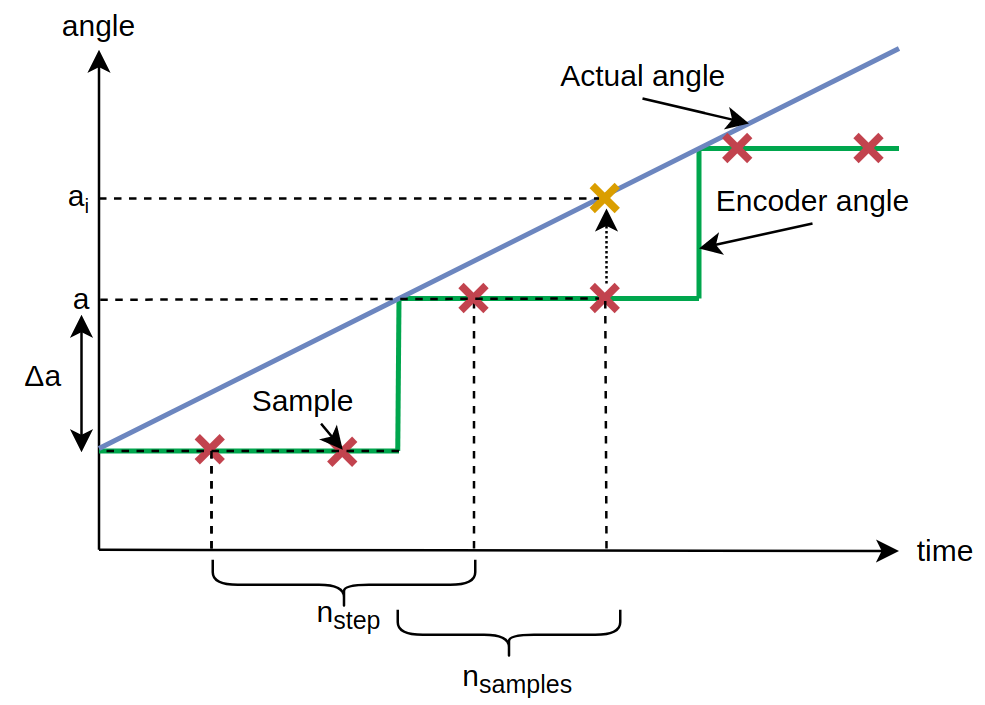
\includegraphics[width=0.8\textwidth]{pictures/software/angle_interpolation2.png}
	\caption{Practical version of linear interpolation.}
	\label{fig:angle_interpolation2}
\end{figure}






% The motor maximum speed is $5000RPM$ so the interpolation should be able to handle steps being skipped.

Equation \ref{eq:linear_interpolation3} can be rewritten to have the two counters as the fraction resulting in equation \ref{eq:linear_interpolation}.
\begin{equation}
a_{i} =  \frac{n_{samples}}{n_{step}} \Delta a  + a
\label{eq:linear_interpolation}
\end{equation}

$n_{samples}$ are a count of the number of samples on the current step. The counter starts at $0$ which means $n_{samples} \leq n_{steps}$ if the speed is approximately the same for the current and last encoder step.

\begin{equation}
	0 \leq	\Big(\frac{n_{samples}}{n_{step}} \Big) \leq 1
\end{equation}
Which means that the output of the interpolation is limited to
\begin{equation}
	 a \leq a_i \leq (a + \Delta a)
\end{equation}


The finished interpolation algorithm can be seen in the code snippet \ref{code:interpolation_algorithm} below. 

Every time the function is called a counter, \textit{time}, is incremented and this counter keeps track of the time.

Line $5$ to $8$ handle the first time the interpolation is used and it updates the variable $t\textunderscore 1$ which is the time of the left edge of the counter $n_{step}$. 

Line $10$ to $15$ handles the interpolation until the right edge of $n_{step}$ is updated, this is done with the variable $t\textunderscore 2$. For both the edges the value from the encoder is saved from the encoder to handle the step size in case one or more steps are skipped.

Line $17$ to $29$ handle the actual running algorithm. The sample counter is incremented. If a new step is reached the left edge is set the the last right edge, $t\textunderscore 1 = t\textunderscore 2$, and the new right edge is updated, $t\textunderscore 2 = angle$.

The step width is calculated as well as the step size which results in all the variable ready to calculate the interpolated angle on line $28$ as per equation \ref{eq:linear_interpolation}.

\begin{lstlisting}[style=c, caption=Interpolation algorithm implemented on the embedded system., label=code:interpolation_algorithm]
f32 interpolateAngle(f32 angle){
	time++;								                 // Keep track of time
	f32 angleInterpolated = angle;		     // Default value of angle
	/* First time used */
	if(t1 == 0){
		t1 = time;						               // Update time of t1
		t1v = angle;					               // Update angle of t1
	}
	/* If t2 has not been updated for the first time yet */
	if(t2 == 0){
		if(angle != t1v){				             // Check if first step happens
			t2 = time;					               // If so update time for t2
			t2v = angle;				               // Update angle of t2
		}
	}
	/* For all other steps than the first two */
	if(t1 != 0 && t2 != 0){				         // Do the actual interpolation
		nSamples++;						               // Keep track of samples on current step
		if(angle != t2v){				             // If new step happens
			t1 = t2;					                 // Move t2 to t1
			t1v = t2v;					               // Update value of t1
			t2 = time;					               // Update t2 to current time
			t2v = angle;				               // Update value of t2 to current angle
			nSamples = 0;				               // Reset number of samples on step
		}
 		u32 nStep = t2 - t1;				         // Get time on last step (approximation)
		f32 angleStep = t2v-t1v;	           // Get angle step
		angleInterpolated = nSamples/nStep * angleStep + angle; // Calculate new angle
	}
	return angleInterpolated;			         // Return new angle
}
\end{lstlisting}

To measure the improvement of the interpolated angle compared to the encoder angle a sweep of the motor speed from 1RPM to 5000RPM has been performed. The sweep was done with the algorithm implemented in Matlab. The results are shown on figure \ref{fig:interpolation_error}. The interpolated error is smaller for speeds less than $1185RPM$ otherwise the interpolation error is the same as the general error.


\begin{figure}[H]
	\centering
	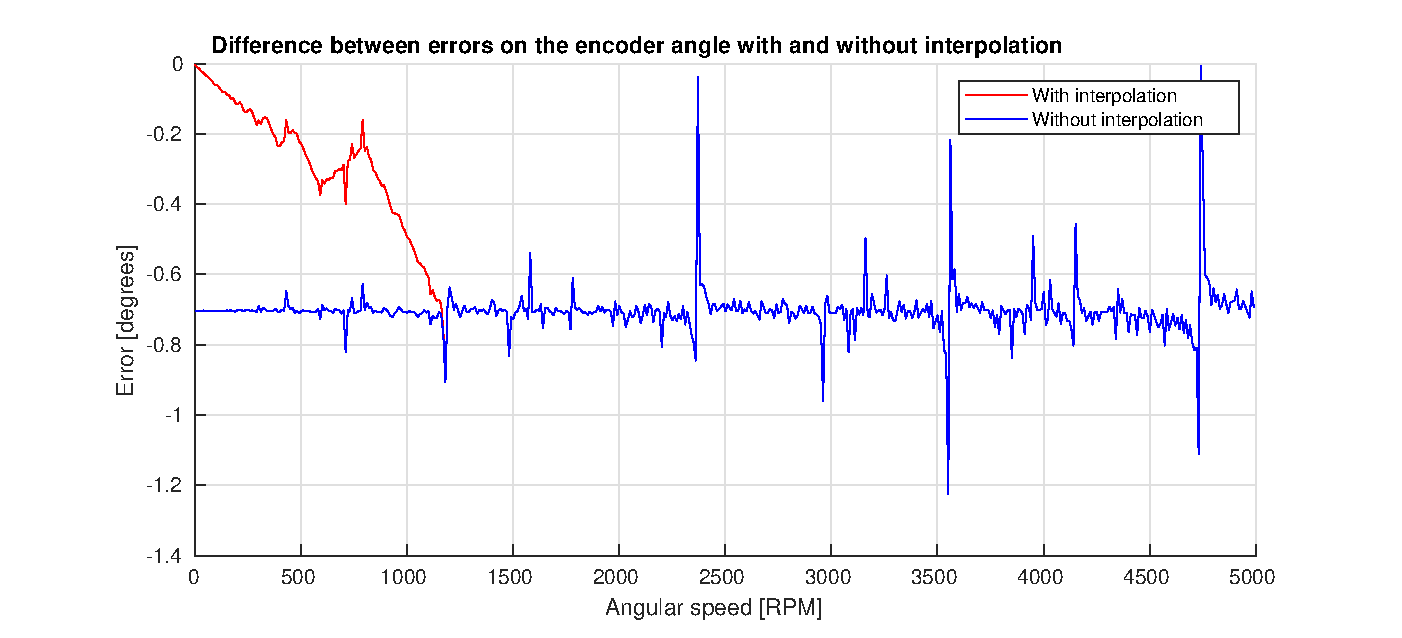
\includegraphics[width=1\textwidth]{pictures/software/interpolation_error.eps}
	\caption{Frequency sweep of angular error with and without linear interpolation.}
	\label{fig:interpolation_error}
\end{figure}


\subsubsection*{Conclusion}
The angle interpolation works to limit the encoder angle error for speeds under $1185RPM$ but speeds over $1185RPM$ the interpolation just follows the normal encoder angle error.

%ADC
\subsection{Analog-to-Digital Converter (ADC)}

To measure the phase currents once per PWM cycle and also the torque reference from the torque pedal an ADC is used. The Zynq has two 12 bit ADCs which enables it to sample two signals simultaneously. It is important to sample the phase current same time to avoid distortion by having a small time delay between current samples. 

Due to the symmetry between the three phases only two of the phases needs to be measured and the last can be caltulated with equation \ref{eq:third_phase}.
\begin{equation}
    I_C = -(I_A + I_B)
    \label{eq:third_phase}
\end{equation}
The calculation of the last phase is done in the processing system.

To control the ADC the IP block \textit{XADC} is used which can be seen on figure \ref{fig:adc_module}. 

\begin{figure}[H]
	\centering
	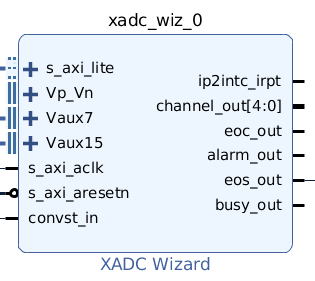
\includegraphics[width=0.35\textwidth]{pictures/software/adc.png}
	\caption{IP core to handle the two ADC in the Zynq.}
	\label{fig:adc_module}
\end{figure}

The block is configured to be triggered by an external signal which is connected to one of the ADC pulses produced by a PWM module.

While the phase currents are measured the torque pedal position is also measured. When all signals are measured the signal end-of-sequence, \textit{eos\textunderscore out}, outputs a pulse. The \textit{eos} signal is used to trigger the interrupt on the processing system as can be seen on figure \ref{fig:adc_block_diagram}.

\begin{figure}[H]
	\centering
	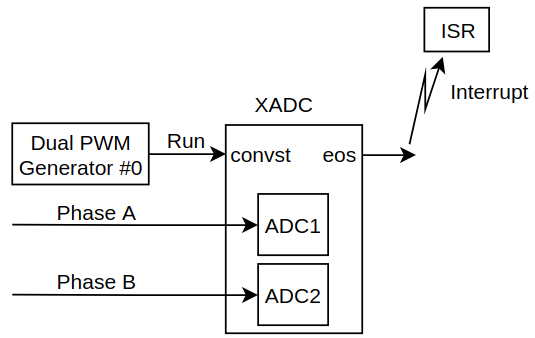
\includegraphics[width=0.5\textwidth]{pictures/software/adc_block_diagram.png}
	\caption{Function diagram showing the signals in and out of the ADC module.}
	\label{fig:adc_block_diagram}
\end{figure}





\subsubsection*{Subconclusions}
A dual PWM module is developed that can produce two individual and inverted PWM signals with dead time and ADC trigger pulses. Tests show that three of these modules can be used at the same time phase shifted $120\circ$. The encoder module IP is included and a higher level algorithm is developed to improve the readings. Lastly the ADCs in the Zynq is imported and configured.

%%%%%%%%%%%%%%%%%%%%% PS %%%%%%%%%%%%%%%%%%%%%
\subsection{Processing System (PS)}
All the high level control and communication is placed on the processing system to get the benefit of higher abstraction on a processor. The section is structured in the same way as data is processed. First the ISR and how the PL triggers the PS, then the control and lastly how the result is transferred back to the PL. The section will end with the communication interface between the embedded system and a computer.


% Interrupt Service Routine ISR
\subsubsection{Interrupt Service Routine}
\label{sec:isr}
Every time an interrupt is triggered the ISR is called which sends a run command to the control loop to run. The interrupts are triggered with the same frequency as the PWM is running with, which is $10kHz$. Normal running behavior could look like the scenario shown on figure \ref{fig:isr1}. 

\begin{figure}[H]
	\centering
	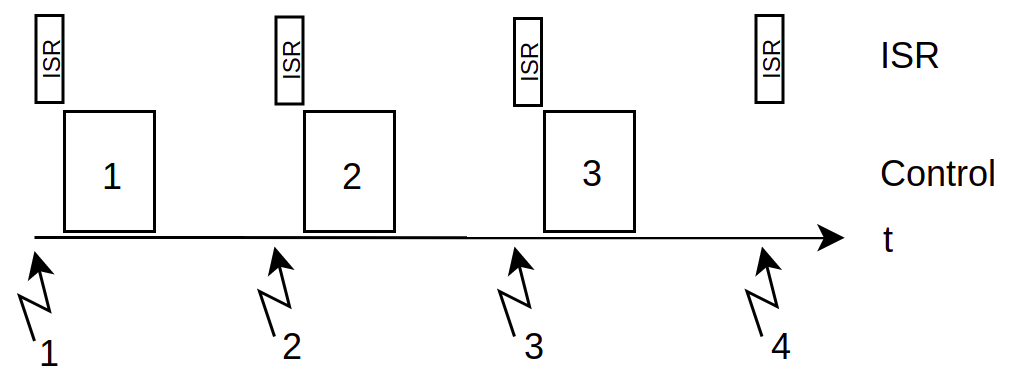
\includegraphics[width=0.65\linewidth]{pictures/software/isr/isr1.png}
	\caption{Normal running behavior of the interrupts coming in triggering the ISR which then triggers the control loop task.}
	\label{fig:isr1}
\end{figure}

Every time an interrupt is received the control loop is run and there is always some time between the control is run where the processor is idle.


The unlikely case where the control takes more time than the time between two interrupts can be seen in figure \ref{fig:isr2}. For robustness the system should be able to handle this situation. 

If the run command used by the ISR to trigger the control is a simple boolean variable set high by the ISR and reset as the first step in the control loop it is possible to get an interrupt while executing control. The running control will then finish and the new request will directly start executing.

\begin{figure}[H]
	\centering
	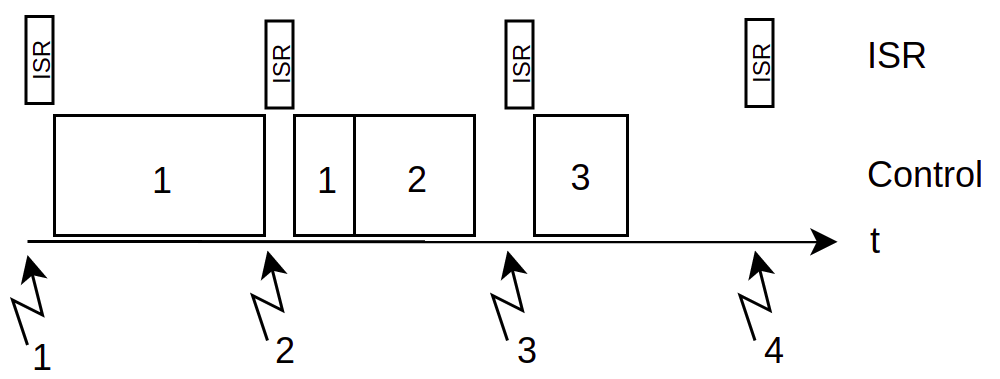
\includegraphics[width=0.65\linewidth]{pictures/software/isr/isr2.png}
	\caption{Unlikely scenario where a control task takes longer than the time between two interrupts.}
	\label{fig:isr2}
\end{figure}

Problems arise from this solution if the very unlikely event happen where multiple interrupts happen during the same control loop cycle as can be seen on figure \ref{fig:isr4}. Every interrupt before the last will be overlooked. In some systems overseeing an interrupt can be catastrophic but in this case it will improve the performance of the system compared to the alternative of executing all control tasks as can be seen on figure \ref{fig:isr3}.

\begin{figure}[H]
	\centering
	\includegraphics[width=0.65\linewidth]{pictures/software/isr/isr4.png}
	\caption{The scenario of a control task running for much longer than expected and skipping interrupts.}
	\label{fig:isr4}
\end{figure}

\begin{figure}[H]
	\centering
	\includegraphics[width=0.65\linewidth]{pictures/software/isr/isr3.png}
	\caption{The scenerio of a control task running for much longer than expected but no interrupts are overseen.}
	\label{fig:isr3}
\end{figure}


Executing every control task will result in the system handling old data which is not relevant anymore. 

Therefore the run command used by the ISR to trigger the control loop is a simple boolean variable.

% Clarke Park
\subsubsection{Clarke Transformation and Park Transformation}
The control type chosen for the system is vector control also called field-oriented control and this requires Clarke/Park transformations as well as their inverse counterparts.
The transformations are implemented in the processing system and to limit the amount of calculations needed for each transformation all constants are defined beforehand.

% ******* Clarke Transformation ***********************************
\subsubsection*{Clarke Transform}


The embedded implementation of the Clark transformation as per equation \ref{eq:clarke_transformation} can be seen in code sample \ref{code:clarke}. The function creates two results and therefore instead of returning the values, the variables are declared outside the function calls and a pointer to the variables are parsed into the function.

\begin{lstlisting}[style=c, caption=Embedded Clarke Transformation., label=code:clarke]
/* The Clarke function */
void clarke(f32 *iAlpha, f32 *iBeta, f32 iA, f32 iB, f32 iC){
	*iAlpha = TWO_THIRDS * iA - ONE_THIRD * iB - ONE_THIRD * iC;
	*iBeta  = ONE_OVER_SQRT_THREE * iB - ONE_OVER_SQRT_THREE * iC;
}
\end{lstlisting}

% ************** Park Transformation ***********************************
\subsubsection*{Park Transform}
The embedded implementation of the Park transformation as per equation \ref{eq:park_transformation} can be seen in code sample \ref{code:park}. The transformation involves calculating the sine and cosine of the angle. These two functions are implemented by using look-up tables and are discussed in section \ref{sec:sine_cosine}.

\begin{lstlisting}[style=c, caption=Embedded Park Transformation., label=code:park]
/* The Park function */
void park(f32 *iD, f32 *iQ, f32 iAlpha, f32 iBeta, f32 angle){
	const f32 cosAngle = fastCos(angle);
	const f32 sinAngle = fastSin(angle);
	*iD = cosAngle * iAlpha + sinAngle * iBeta;
	*iQ = -sinAngle * iAlpha + cosAngle * iBeta;
}
\end{lstlisting}

The inverse Clarke and inverse Park transformations can be found in appendix \ref{app:inverse_park} and \ref{app:inverse_clarke}.


\paragraph{Sine and Cosine}
\label{sec:sine_cosine}
The trigonometric functions sine and cosine are implemented with a look-up table to improve performance. The sine function looks up a given angle in the table to find the output of the function. The cosine uses the sine function but offset the angle by $90 ^{\circ}$. 

To limit the amount of memory used only one value is saved per degree which results in $360$ saved values of type \textit{f32} which is based on the type \textit{float}. The variables are $4$ bytes resulting in $1440 bytes \sim 1.5kB$ used.
The maximum error that can exist because of the quantization is the biggest step between two values in the data set. 
The largest error is where the sine/cosine has the largest slope, and this is where it crosses 0 on the y-axis. The error is positive when the slope is positive and negative when the slope is negative. The maximum error is $\pm 1.75 \%$ as can be seen on figure \ref{fig:sinus_lookup_error}. 
\begin{figure}[H]
	\centering
	\includegraphics[width=0.6 \textwidth]{pictures/software/sinus_lookup_error.eps}
	\caption{Error between the real sine value and the look-up table value.}
	\label{fig:sinus_lookup_error}
\end{figure}



\begin{lstlisting}[style=c, caption=Sine and cosine implemented with look-up tables., label=code:lookup_table]
/* Sine lookup table */
#define SIN_N 		360	 // Number of data points in the sine constant array
const f32 sineValues[] = {0,0.0174524064372835,0.0348994967025010,...};

/* Function that returns sin(angle) */
f32 fastSin(f32 angle){
	unsigned int index = (unsigned int)angle;       // Truncate decimals
	return (f32)sineValues[index % SIN_N];      // 
}	

/* Function that returns cos(angle) */
f32 fastCos(f32 angle){
	f32 newAngle = (f32)((int)(angle + 90) % (int)360);
	return (f32)fastSin(newAngle);
}
\end{lstlisting}

% Controller
\subsubsection{Controller}
\label{sec:embedded_control}
The PI-controller is implemented in \textit{c} on the processing system in a object orientated way where each of the two controllers are defined together with their gains. When the system is booted up the controllers are initialized with the values and prepared for usage. The code for this can be seen in code sample \ref{code:pi_controller1}.

\begin{lstlisting}[style=c, caption=Initialization of PI-controller., label=code:pi_controller1]
/* Declare controllers */
Controller cQ, cD;
static f32 kpQ = 1, kiQ = 1, kpD = 1, kiD = 1;

void initControllers(){
    /* Initialize controllers with gains */
    initController(&cQ, kpQ, kiQ);
    initController(&cD, kpD, kiD);
}
\end{lstlisting}

When the motor is running the only thing needed to be done is to input the reference value and the current measured value to the controller and get a new output as can be seen in code sample \ref{code:pi_controller2}. The function 'getOutput()' handles the controller gains, keeping track of the integrator part and integrator windup.

\begin{lstlisting}[style=c, caption=Usage of PI-controller., label=code:pi_controller2]
    /* Run controller */
	f32 outD = getOutput(&cD, 0, iD);
	f32 outQ = getOutput(&cQ, getTargetTorque(), iQ);
\end{lstlisting}

The implementation of the 'getOutput()' function can be seen in code sample \ref{code:pi_controller3}.
First the controller gains \textit{kp} and \textit{ki} are retrieved. Then the controller's integrator part is updated and then retrieved.

The output of the controller is found with the following equation.
\begin{equation}
    u = k_p \cdot e + k_i \cdot int
\end{equation}

Where $u$ is the output, $e$ is the error which is the target minus the input, 

$e = target - input$, $int$ is the integrator part and $k_p$ and $k_i$ are the controller gains.

The integral part of the controller might experience integrator windup because the control execution is much faster than the motor acceleration. To handle this a simple output limitation is implemented to limit the controller output.



\begin{lstlisting}[style=c, caption=Implementation of PI-controller 'get output'-function., label=code:pi_controller3]
/* Function to get the next output of a controller with a new input */
f32 getOutput(Controller *c, f32 target, f32 input){
	f32 error = target - input;                         // Calculate error
	
	// Collect controller data
	const f32 kp  = getKp(c);
	const f32 ki  = getKi(c);
	addToIntegrator(c, error);
	const f32 integrator = getIntegrator(c);

	f32 output =  (kp * error) + (ki * integrator);     // Calculate new output
	
	// Anti integrator windup. Limit the output to within set limits
	if(output > MAX_OUTPUT){                            // Check upper limit
		output = MAX_OUTPUT;                              // Limit output
	}
	if(output < MIN_OUTPUT){                            // Check lower limit
		output = MIN_OUTPUT;                              // Limit output
	}	
	return output;                                      // Return new output
}
\end{lstlisting}



% Communication between PL and PS
\subsection{Communication between PL and PS}
Sending thresholds from the processing system to the PWM low-level modules are done through a piece of block RAM.
The build-in block RAM of the Zybo consist of a 36kbit storage area with two independent access ports. 

The PWM modules expect 8 bit thresholds which results in 24 bits or 3 bytes being used of the block RAM. 

A mere 3 bytes account for around $0.08\%$ of the total block RAM. While this is a waste of the block RAM, it was chosen because of it being easily accessible from both the PS and PL and easy to set up. 

When the control task on the processing system has run and produced the thresholds for each phase they are written into the first 3 bytes of the block RAM as can be seen on figure \ref{fig:com_pl_to_ps}.

\begin{figure}[H]
	\centering
	\includegraphics[width=1\linewidth]{pictures/software/com_pl_to_ps.png}
	\caption{Communication from PS to PL through block RAM.}
	\label{fig:com_pl_to_ps}
\end{figure}

From here the memory interface module in the logic can collect the thresholds and parse them unto the three PWM modules as can be seen on figure \ref{fig:com_pl}. The PWM modules then use the thresholds to produce the PWM signals as discussed in section \ref{sec:pwm}.


\begin{figure}[H]
	\centering
	\includegraphics[width=0.8\linewidth]{pictures/software/com_pl.png}
	\caption{The data flow in the PL from the block RAM to the PWM generators.}
	\label{fig:com_pl}
\end{figure}




% Computer inteface
\subsection{Computer interface}

To keep track of the system, start the converter and change the gains for the controllers an interface between the embedded controller and a computer is made. The interface is made in a simple low-level way with a predefined message structure and limited error handling. The structure can be seen in table \ref{tab:message_structure}. 


\begin{table}[H]
\centering
\begin{tabular}{|l|c|c|c|c|c|c|}
\hline
\# character       & 1       & 2                 & 3            & 4            & 5       & 6   \\ \hline
Function      & ID  & Read / Write                     & \multicolumn{4}{c|}{Value}               \\ \hline
Valid Values & $0\rightarrow 9$ & 'r'/'w'  & \multicolumn{4}{c|}{$0\rightarrow 9999$} \\ \hline
\end{tabular}
\caption{Structure of the interface messages from the computer to the embedded controller.}
\label{tab:message_structure}
\end{table}

The first character of the message contains an ID of the variable that the message is referring to. The IDs of all variables included can be seen in table \ref{tab:variable_ids}.

The second character describes if the message is a read or write command.

The third till sixth character are only used for the write command. They contain the value to which the variable from the second character should be changed to. The format of the value can be seen in table \ref{tab:variable_ids}. To be able to handle digits the gains send as values from $0000 \rightarrow 9999$ but in the controller these are mapped to $00.00 \rightarrow 99.99$.


\begin{table}[H]
\centering
\begin{tabular}{|l|llll|} \hline
ID & Valid values                                               & Valid commands & Variable    & Unit       \\   \hline
0  & \begin{tabular}[c]{@{}l@{}}0 = Stop\\1 = Run \end{tabular} & 'r'/'w'        & Inverter state & - \\ \hline
1  & -                                                          & 'r'            & Speed       & Hz \\ \hline
2  & $0 \rightarrow 9999$                                                     & 'r'/'w'        & Ki\_D       & \begin{tabular}[c]{@{}l@{}}$1/100$ \\ \textit{Example: 1234 = 12.34}\end{tabular} \\ \hline
3  & $0 \rightarrow 9999$                                                     & 'r'/'w'        & Kp\_D       & \begin{tabular}[c]{@{}l@{}}$1/100$ \\ \textit{Example: 1234 = 12.34}\end{tabular} \\ \hline
4  & $0 \rightarrow 9999$                                                     & 'r'/'w'        & Ki\_Q       & \begin{tabular}[c]{@{}l@{}}$1/100$\\ \textit{Example: 1234 = 12.34}\end{tabular}  \\ \hline
5  & $0 \rightarrow 9999$                                                     & 'r'/'w'        & Kp\_Q       & \begin{tabular}[c]{@{}l@{}}$1/100$\\ \textit{Example: 1234 = 12.34}\end{tabular}  \\ \hline
\end{tabular}
\caption{List of variables that can be accessed through the communication between a computer and the embedded controller.}
\label{tab:variable_ids}
\end{table}

An example of how the communication can be seen on figure \ref{fig:pc_interface}. 

Line 1 is a command to write the value $03.46$ to \textit{Ki\textunderscore D}. 

Line 2 is a read command of the same variable. 

Line 3 is the reply from the embedded system.

Line 5 is a write command to start the inverter. Line 6 and 7 are the same as 2 and 3 but for the inverter state.

Line 9 is a command to write the value $15.23$ to the gain \textit{Ki\textunderscore Q}.

\begin{figure}[H]
	\centering
	\includegraphics[width=0.65\linewidth]{pictures/software/pc_interface_terminal.png}
	\caption{Example of the computer interface used for communication between the embedded controller and a computer.}
	\label{fig:pc_interface}
\end{figure}

\subsubsection*{Subconclusions}
A short ISR is developed to simply trigger the actual control loop in the processor. When the control is triggered it runs Clarke and Park Transformations, angle interpolation, and two PI controllers. The controller output is then converted back into PWM thresholds with an Inverse Park and Inverse Clarke transformation and the result is put into block RAM for the PL to use.





\newpage
% Discussion
\section{Discussion}

\newpage
% Conclusion
\section{Conclusion}
\label{sec:conclusion}



The three-phase inverter was designed with the requirements of an electric go-kart in mind. 

As price was the primary concern the smallest possible PCB area was desirable which brought other trade-offs. 
To minimize the size of the power and driver boards and in turn improve the overall modularity, the PCB's were made to only handle one phase and three boards were then used to handle the three-phases.
For power board an aluminum PCB was used to have a high heat conductivity which allows for the use of SMD MOSFET's as the high power transistors. The driver board was build to be mounted directly on top of the power board to minimize driver signal path lengths and parasitic inductances.

The motor is controlled on the Zynq with a PI controller in a field orientated way. Each phase is controlled with a dual PWM module with deadtime between the two PWM signals implemented in the FPGA.
The angle out of the encoder has a low resolution so a more accurate angle is approximated at low speeds with the use of a linear interpolation algorithm. 

Since the inverter was not built it is not possible to back up the theoretical work.

It was not possible to make a fully working model of a controlled motor. A tuned discrete controller was therefore not implemented in the project.

% The theoretical motor controller should be able to control the \textit{ME1117 PMAC motor}, the controller has been made on a Zynq FPGA and a inverter has been designed with control. 
% The Zynq FPGA design is able give relevant data through communication interface on a computer. 
% All this is done with out change any of the existing components, but without a finished build the cost requirement also left unchecked.

\newpage
% Missing features
\section{Missing features and future work}
\label{sec:missing_features}

\newpage
% Litterature

\newpage
% Symbol list
\section{Symbol list}
\label{sec:symbol_list}

\begin{center}
\begin{tabular}{|c|c|c|} \cline{1-3}
\textbf{Symbol name} & \textbf{Symbol} & \textbf{Unit} \\ \cline{1-3}
\textbf{Unitless} & \dots & \dots \\ \cline{1-3}
\textbf{Danish krones} & $dkk$ & \textit{kroner} \\ \cline{1-3}
\textbf{Voltage} & $V$ & \textit{Volts} \\ \cline{1-3}
\textbf{Ampere} & $A$ & \textit{Amps} \\ \cline{1-3}
\textbf{Resistance} & $\Omega$ & \textit{Ohms} \\ \cline{1-3}
\textbf{Coil} & $L$ & \textit{Henry} \\ \cline{1-3}
\textbf{Capacitor} & $C$ & \textit{Farad} \\ \cline{1-3}
\textbf{Frequency} & $f$ & $Hz$\\ \cline{1-3} 
\textbf{Rotational speed} & $N$ & \textit{RMP}\\ \cline{1-3}
\textbf{Pole pair} & $P$ & \dots \\ \cline{1-3}
\textbf{Time} & $s$ & \textit{seconds} \\ \cline{1-3}
\textbf{Electrical degrees} & $\circ$ & \textit{Degrees} \\ \cline{1-3}
\end{tabular} \\
\caption{Symbol list}\label{Symbollist}
\label{tab:variable_ids}
\end{center}


\newpage
% Abbreviation list
\section{Abbreviation list}
\label{sec:abbreviation_list}

% abcdefghijklmnopqrstuvwxyz
\begin{table}[H]
\centering
\begin{tabular}{|r|l|}
\hline
\textbf{Abbreviation} & \textbf{Meaning}                                        \\ \hline
AC           & Alternating Current                                              \\ \hline
ADC          & Analog to Digital Conversion                                     \\ \hline
AXI          & Advanced eXtensible Interface                                    \\ \hline
BLDC         & Brush Less DC Motor                                              \\ \hline
CMRR         & Common-Mode Rejection Ratio                                      \\ \hline
CSI          & Common Source Inductance                                         \\ \hline
DC           & Direct Current                                                   \\ \hline
EOS          & End Of Sequence                                                  \\ \hline
FET          & Field-Effect Transistor                                          \\ \hline
FOC          & field oriented control                                           \\ \hline
FPGA         & Field-Programmable Gate Array                                    \\ \hline
IP           & Intellectual Property (Block)                                    \\ \hline
ISR          & Interrupt Service Routine                                        \\ \hline
MOSFET       & Metal-Oxide-Semiconductor Field-Effect Transistor                \\ \hline
PCB          & Printed Circuit Board                                            \\ \hline
PI           & Proportional Integral (Controller)                               \\ \hline
PL           & Programmable Logic                                               \\ \hline
PMAC         & Permanent Magnet AC Motor                                        \\ \hline
PMSM         & Permanent Magnet Synchronous Motor                               \\ \hline
PS           & Processing System                                                \\ \hline
PWM          & Pulse-Width Modulation                                           \\ \hline
RAM          & Random Access Memory                                             \\ \hline
SDU          & University of Southern Denmark                                   \\ \hline
SMD          & Surface Mount Device                                             \\ \hline
UART         & Universal Asynchronous Receiver/Transmitter                      \\ \hline
VHDL         & Very high speed integrated circuit Hardware Description Language \\ \hline
             &                                                                  \\ \hline
\end{tabular}
\caption{Abbreviation list}\label{Abbreviationlist}
\label{tab:variable_ids}
\end{table}


\newpage
\listoffigures

\newpage
% References
\section{References}

%to use the Reference \cite{Name of the source},

\begin{thebibliography}{9}
\bibitem{Project 1. semester - S19} 
Project 1. semester - S19 - Electronics - ver1.pdf, \\
Karsten Holm Andersen, (2019)

\bibitem{Motor_Parameters}
http://www.motenergy.com/me1117.html
Parameters taken from the production desciption
Motenergy \copyright 2011
 

\end{thebibliography}

\newpage
% Appendix
\section{Appendix}
\label{sec:appendix}
\appendix
% Code samples
\section{Code Samples}
\label{app:code_samples}
The appendix contains code samples from various important and interesting sections of the program code implemented on the Xilinx Zynq controller.

% ************************** Clarke Transformation ***********************************
\subsection{Clarke / Park Transformations}
\subsubsection*{Clarke Transformation}
\label{app:clark}
The embedded implementation of the Clarke Transformation.

\begin{lstlisting}[style=c, caption=Embedded Clarke Transformation., label=app:code:clarke]
/* The Clarke function */
void clarke(f32 *iAlpha, f32 *iBeta, f32 iA, f32 iB, f32 iC){
	*iAlpha = TWO_THIRDS * iA - ONE_THIRD * iB - ONE_THIRD * iC;
	*iBeta  = ONE_OVER_SQRT_THREE * iB - ONE_OVER_SQRT_THREE * iC;
}
\end{lstlisting}

% ************************** Park Transformation ***********************************
\subsubsection*{Park Transformation}
\label{app:park}
The embedded implementation of the Park Transformation.
\begin{lstlisting}[style=c, caption=Embedded Park Transformation., label=app:code:park]
/* The Park function */
void park(f32 *iD, f32 *iQ, f32 iAlpha, f32 iBeta, f32 angle){
	const f32 cosAngle = fastCos(angle);
	const f32 sinAngle = fastSin(angle);
	*iD = cosAngle * iAlpha + sinAngle * iBeta;
	*iQ = -sinAngle * iAlpha + cosAngle * iBeta;
}
\end{lstlisting}


% ************************** Inverse Park Transformation ***********************************
\subsubsection*{Inverse Park Transformation}
\label{app:inverse_park}
The embedded implementation of the Inverse Park Transformation.

\begin{lstlisting}[style=c, caption=Embedded Inverse Park Transformation., label=app:code:inverse_park]
/* The inverse Park function */
void invPark(f32 *iAlpha, f32 *iBeta, f32 iD, f32 iQ, f32 angle){
	const f32 cosAngle = fastCos(angle);
	const f32 sinAngle = fastSin(angle);
	*iAlpha = cosAngle * iD - sinAngle * iQ;
	*iBeta  = sinAngle * iD + cosAngle * iQ;
}
\end{lstlisting}



% ************************** Inverse Clarke Transformation ***********************************
\subsubsection*{Inverse Clarke Transformation}
\label{app:inverse_clarke}
The embedded implementation of the Inverse Clarke Transformation.

\begin{lstlisting}[style=c, caption=Embedded Inverse Clarke Transformation., label=app:code:inverse_clarke]
/* The inverse Clarke function */
void invClarke(f32 *iA, f32 *iB, f32 *iC, f32 iAlpha, f32 iBeta){
	*iA = iAlpha;
	*iB = -HALF * iAlpha + SQRT_THREE_OVER_TWO * iBeta;
	*iC = -HALF * iAlpha - SQRT_THREE_OVER_TWO * iBeta;
}
\end{lstlisting}


\subsection{Encoder}
\subsubsection{Read rotor angle}
The code in to read out a rotor position and convert it to degrees.
\label{app:readRotorAngle}
\begin{lstlisting}[style=c, caption=Function to read an angle from the encoder. The angle is returned in degrees. label=app:code:getRotorAngle]
/* Read the rotor angle */
f32 getRotorAngle(){
    u8 position = RM28MD_POSITION & 0x000000FF;     // Only the first byte is valid
    f32 angle   = 359/255 * position;       	      // Map position (0->255) to 
                                                    // angle (0->359)
    return angle;                                   // Return angle
}
\end{lstlisting}

\subsubsection{Linear Interpolation}
The linear interpolation algorithm as discussed in section \ref{sec:linear_interpolation}. The algorithm takes in low resolution encoder angles and depending on the time between encoder angle changes the readings are used to approximate a more accurate angle.
\begin{lstlisting}[style=c, caption=Implemetation of angle intepolation algorithm., label=app:code:interpolateAngle]
/* Linear Interpolation Algorithm */
f32 interpolateAngle(f32 angle){
	time++;								                 // Keep track of time
	f32 angleInterpolated = angle;		     // Default value of angle
	/* First time used */
	if(t1 == 0){
		t1 = time;						               // Update time of t1
		t1v = angle;					               // Update angle of t1
	}
	/* If t2 has not been updated for the first time yet */
	if(t2 == 0){
		if(angle != t1v){				             // Check if first step happens
			t2 = time;					               // If so update time for t2
			t2v = angle;				               // Update angle of t2
		}
	}
	/* For all other steps than the first two */
	if(t1 != 0 && t2 != 0){				         // Do the actual interpolation
		nSamples++;						               // Keep track of samples on current step
		if(angle != t2v){				             // If new step happens
			t1 = t2;					                 // Move t2 to t1
			t1v = t2v;					               // Update value of t1
			t2 = time;					               // Update t2 to current time
			t2v = angle;				               // Update value of t2 to current angle
			nSamples = 0;				               // Reset number of samples on step
		}
 		u32 nStep = t2 - t1;				         // Get time on last step (approximation)
		f32 angleStep = t2v-t1v;	           // Get angle step
		angleInterpolated = nSamples/nStep * angleStep + angle; // Calculate new angle
	}
	return angleInterpolated;			         // Return new angle
}
\end{lstlisting}

\newpage
\subsection{Control}
\subsubsection{PI Controller}
The code for determining the next output value of the PI controller. The function takes in a controller, a target value and an input. It then calculates the controller output from its gains and integrator. The function includes integrator windup limitation. The section discussing the controller can be found in section \ref{sec:embedded_control}.
\begin{lstlisting}[style=c, caption=Implementation of the embedded PI controller., label=app:code:sineAndCosine]
/* Function to get the next output of a controller with a new input */
f32 getOutput(Controller *c, f32 target, f32 input){
	f32 error = target - input;                         // Calculate error
	
	// Collect controller data
	const f32 kp  = getKp(c);
	const f32 ki  = getKi(c);
	addToIntegrator(c, error);
	const f32 integrator = getIntegrator(c);

	f32 output =  (kp * error) + (ki * integrator);     // Calculate new output
	
	// Anti integrator windup. Limit the output to within set limits
	if(output > MAX_OUTPUT){                            // Check upper limit
		output = MAX_OUTPUT;                              // Limit output
	}
	if(output < MIN_OUTPUT){                            // Check lower limit
		output = MIN_OUTPUT;                              // Limit output
	}	
	return output;                                      // Return new output
}
\end{lstlisting}


\subsubsection{Sine and Cosine}
\label{app:sineCosine}
The implemented version of sine and cosine. The two functions are implemented with the help of a look-up table. The section discussing these can be found in section \ref{sec:sine_cosine}.
\begin{lstlisting}[style=c, caption=Sine and cosine implemented with look-up tables., label=app:code:sineAndCosine]
/* Sine lookup table */
#define SIN_N 		360	 // Number of data points in the sine constant array
const f32 sineValues[] = {0,0.0174524064372835,0.0348994967025010,...};

/* Function that returns sin(angle) */
f32 fastSin(f32 angle){
	unsigned int index = (unsigned int)angle;       // Truncate decimals
	return (f32)sineValues[index % SIN_N];      // 
}	

/* Function that returns cos(angle) */
f32 fastCos(f32 angle){
	f32 newAngle = (f32)((int)(angle + 90) % (int)360);
	return (f32)fastSin(newAngle);
}
\end{lstlisting}


\end{document}
